% =====================================================================
%  PAPER A — the benchmark. A verified defect benchmark on AACR-Bench,
%  applied to eight reviewers at their best-shot configurations.
%  Companion: quickreview.tex (the QuickReview technical report).
%
%  DRAFT (2026-09-28; base model, stability and the current-build re-run
%  added 2026-09-30; rewritten 2026-10-01 around the final comparison:
%  every contender at the best configuration found for it, all
%  OpenAI-based reviewers on gpt-6.1-sol). Single file: diagrams are
%  TikZ, the bibliography is inline (no bibtex run needed).
%  Every number is copied from bench/aacr/FULL-BENCHMARK.md,
%  docs/METHODOLOGY.md, docs/THREATS-TO-VALIDITY.md, METRICS.md,
%  RESULTS.md or charts/numbers*.json unless a footnote says otherwise.
%  Gap markers:
%    \NEEDDATA  -- a number we could compute from existing runs/files
%    \NEEDEXP   -- an experiment we have not run
%    \TODO      -- editorial work
% =====================================================================
\documentclass[11pt,a4paper]{article}

\usepackage[utf8]{inputenc}
\usepackage[T1]{fontenc}
\usepackage{lmodern}
\usepackage[margin=2.5cm]{geometry}
\usepackage{booktabs}
\usepackage{graphicx}
\usepackage{xcolor}
\usepackage{array}
\usepackage{tabularx}
\usepackage{amsmath}
\usepackage{enumitem}
\usepackage{tikz}
\usetikzlibrary{arrows.meta,positioning,fit,calc,backgrounds,shapes.geometric}
\usepackage[hidelinks]{hyperref}

\newcommand{\NEEDDATA}[1]{\textcolor{red}{\textbf{[NEED DATA: #1]}}}
\newcommand{\NEEDEXP}[1]{\textcolor{orange}{\textbf{[NEED EXPERIMENT: #1]}}}
\newcommand{\TODO}[1]{\textcolor{blue}{\textbf{[TODO: #1]}}}

\newcommand{\qcr}{QuickReview}
\newcommand{\code}[1]{\texttt{#1}}
\newcommand{\chart}[1]{../charts/#1.jpg}

% diagram styles
\tikzset{
  box/.style={draw, rounded corners=2pt, align=center, font=\small,
    inner sep=4pt, minimum height=2.2em, fill=white},
  agent/.style={box, fill=blue!6},
  data/.style={box, fill=gray!8, sharp corners},
  human/.style={box, fill=orange!10},
  judge/.style={box, fill=green!8},
  flow/.style={-{Stealth[length=2mm]}, thick},
  note/.style={font=\footnotesize\itshape, align=center, text=black!70},
}

\setlist{itemsep=2pt,topsep=4pt}
\setlength{\emergencystretch}{3em}

\title{Measuring whether a code review finds the real defects:\\
\large a verified defect benchmark on AACR-Bench, applied to eight
reviewers at their best-shot configurations}
\author{\TODO{authors and affiliation} \\ Quickchat AI}
\date{Draft of 2026-10-01}

\begin{document}
\maketitle

\begin{abstract}
Code-review benchmarks usually score a generated review by how closely it
reproduces the comments the original pull request received. On
AACR-Bench v1.0, a 200-PR multi-language benchmark from Nanjing
University and Alibaba~\cite{aacrbench}, we find that this answer key
measures something else: on the 145 PRs we checked in full, only 12.8\% of
the reference comments are part of a real defect, at least 80\% of them
were written by AI reviewers (including at least 80 ``human'' references
that are rewritten review-bot comments), and only 31\% of the real
defects we verified appear on the list at all. We build a replacement for
all 185 runnable PRs: a verified answer key of 520 defects (90 high, 145
medium, 285 low severity), each checked against the code by agents that
could not see who raised it, with 3{,}093 rejected candidates kept with
their reasons; and a defect-level judge that reads the whole review and
grades every defect found, partial or missed. Two judges from different
model families agree on 98.7\% of 3{,}640 verdicts (Cohen's $\kappa =
0.97$), and the primary judge agrees with itself on 99.7\%. We also
define a best-shot protocol for comparing tools: each tool's documented
configurations are measured on 40 PRs, one is picked per tool by a rule
fixed in advance, and the pick's own bias is measured on the other 145.
Applied to eight reviewers on one base model (gpt-6.1-sol; Claude Code on
Claude Opus 5.5), the benchmark spreads them from 37\% to 79\% of the
defects, where AACR-Bench's own metric places five of them within 1.8
points of each other. The authors build one of the eight reviewers,
QuickReview, which ranks first (79\%, against 67\% for the strongest
third-party configuration); its lead is in medium- and low-severity
defects and is not established on high-severity ones. We report how the
key's construction could favour it, what we measured about that, and
what remains. The key, the exclusions, the judge prompt and every scoring
script are released.
\end{abstract}


\tableofcontents
\clearpage

% =====================================================================
\section{Introduction}
\label{sec:intro}

Automated code review is now a product category, and several vendors
publish benchmarks of their own~\cite{greptilebench,qodobench,deepsourcebench}.
Most tools publish a
number, and most of those numbers are hard to interpret. Three problems
recur:

\begin{enumerate}
  \item \textbf{The answer key.} A benchmark needs to know what a good
  review of a given pull request should say. Public benchmarks usually
  take this from the comments human (or AI) reviewers left on the original
  PR~\cite{aacrbench,codereviewer,contextcrbench}. Those comments were
  never meant to be a complete or correct list of
  the PR's defects.
  \item \textbf{The matching rule.} A benchmark has to decide whether a
  generated comment ``is'' a reference comment. Rules based on file and
  line position penalise a reviewer that anchors the right finding a few
  lines away, and precision-style scores punish every true comment that
  is not on the list.
  \item \textbf{Who runs the benchmark.} Vendors benchmark their own
  tools, and tune them on the benchmark. Numbers that are not separated
  into tuned and unseen data, and that do not state how the answer key
  was built, cannot be checked.
\end{enumerate}

We ran into all three. We build \qcr{}\footnote{\qcr{} is the public
name of the system; its code, configuration and earlier reports call it
\code{quickreviewd}.}, a production reviewer for our own repositories, and
wanted to know whether it finds the problems a careful senior reviewer
would raise before merge. AACR-Bench~\cite{aacrbench} is the most suitable
public benchmark we found: 200 real PRs from open-source repositories in
ten languages and 50 repositories, with a published, runnable
harness~\cite{aacrrepo}. When we scored \qcr{}
with it, the numbers were low for every reviewer and did not track what
we saw reading the reviews. Early prompt iterations raised AACR F1 by
about 20\% while the number of real defects found did not move
(Section~\ref{sec:disagree}). That is what led us to build a second
metric.

This paper reports the benchmark we built in response, and its first
full application. We replace the reference list with a verified defect
key for all 185 runnable PRs, grade reviews with a defect-level judge
checked across two model families, and compare tools with a best-shot
protocol that gives each one the strongest configuration its own
documentation ships or recommends (Figure~\ref{fig:howitworks}). We then
apply it to eight reviewers on one base model, one of which is ours. We
record the reasoning behind each methodological choice, including the
choices we rejected, so that a reader can judge whether the method
favours our own system. It does in several places, and we say where. Our
reviewer's design and the studies that concern only it are in a
companion report~\cite{qcrreport}.

\begin{figure}[t]
\centering
\resizebox{\textwidth}{!}{%
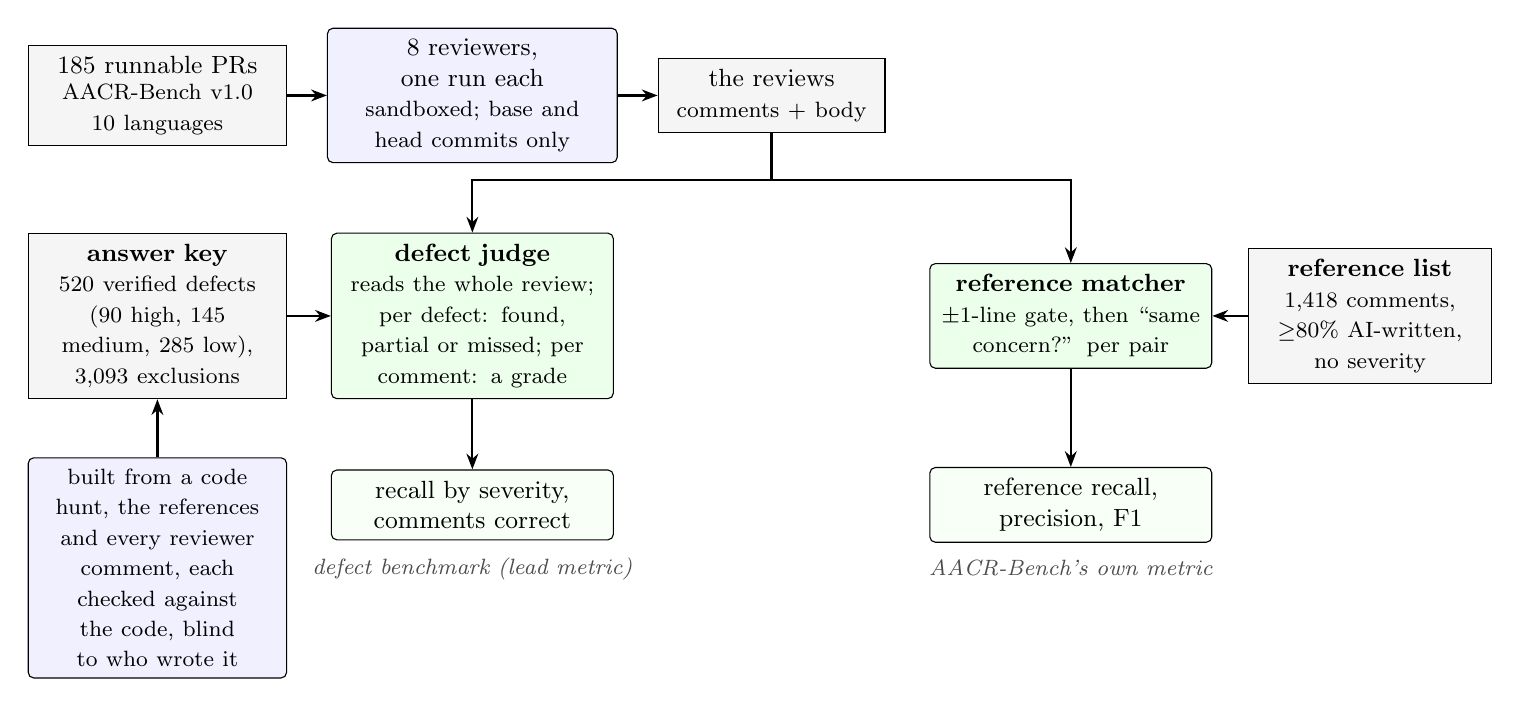
\begin{tikzpicture}
  \node[data, text width=3.0cm] (prs) at (0,0) {185 runnable PRs\\ \footnotesize AACR-Bench v1.0\\ 10 languages};
  \node[agent, text width=3.4cm] (rev) at (4.0,0) {8 reviewers, one run each\\ \footnotesize sandboxed; base and head commits only};
  \node[data, text width=2.6cm] (out) at (7.8,0) {the reviews\\ \footnotesize comments + body};
  \draw[flow] (prs) -- (rev);
  \draw[flow] (rev) -- (out);

  \node[judge, text width=3.3cm] (dj) at (4.0,-2.8) {\textbf{defect judge}\\ \footnotesize reads the whole review; per defect: found, partial or missed; per comment: a grade};
  \node[judge, text width=3.3cm] (aj) at (11.6,-2.8) {\textbf{reference matcher}\\ \footnotesize $\pm1$-line gate, then ``same concern?'' per pair};
  \draw[flow] (out.south) -- ++(0,-0.6) -| (dj.north);
  \draw[flow] (out.south) -- ++(0,-0.6) -| (aj.north);

  \node[data, text width=3.0cm] (key) at (0,-2.8) {\textbf{answer key}\\ \footnotesize 520 verified defects (90 high, 145 medium, 285 low), 3{,}093 exclusions};
  \node[data, text width=2.8cm] (refs) at (15.4,-2.8) {\textbf{reference list}\\ \footnotesize 1{,}418 comments, $\ge$80\% AI-written, no severity};
  \draw[flow] (key) -- (dj);
  \draw[flow] (refs) -- (aj);

  \node[box, fill=green!3, text width=3.3cm] (m1) at (4.0,-5.2) {recall by severity,\\ comments correct};
  \node[box, fill=green!3, text width=3.3cm] (m2) at (11.6,-5.2) {reference recall,\\ precision, F1};
  \draw[flow] (dj) -- (m1);
  \draw[flow] (aj) -- (m2);
  \node[note, below=1mm of m1] {defect benchmark (lead metric)};
  \node[note, below=1mm of m2] {AACR-Bench's own metric};

  \node[agent, text width=3.0cm] (gt) at (0,-6.0) {\footnotesize built from a code hunt, the references and every reviewer comment, each checked against the code, blind to who wrote it};
  \draw[flow] (gt) -- (key);
\end{tikzpicture}}
\caption{How the benchmark works. Every review is scored twice: by our
defect judge against a verified answer key (left; the lead metric) and by AACR-Bench's own reference-comment metric (the
benchmark's published score). Section~\ref{sec:gt} builds the key,
Section~\ref{sec:judging} the judge.}
\label{fig:howitworks}
\end{figure}

\paragraph{Contributions.}
\begin{itemize}
  \item A verified defect answer key for all 185 runnable AACR-Bench v1.0
  PRs (520 defects with severity, evidence, and 3{,}093 recorded
  exclusions\footnote{Sum of the \code{excluded} lists of the five
  committed defect files: 403 on the original 40 PRs and 2{,}690 on
  rest145 (2{,}118 from the v1 build plus 572 from the v2 extension).
  Computed from \code{bench/aacr/defects/*.json}, 2026-09-28.}), built with an
  anonymised, adversarially checked pipeline, and the prompts that built
  it.
  \item A defect-level judge protocol, run on two model families, with
  per-verdict agreement and judge self-consistency reported.
  \item A best-shot protocol for comparing tools: each third-party tool's
  documented configurations measured on 40 PRs that no tuning touched, a
  selection rule fixed before the runs, and the selection's own bias
  measured on the other 145 PRs.
  \item An eight-reviewer comparison on one base model under both the
  benchmark's own metric and the defect metric, with cost and tokens, and
  worked examples of what each severity class looks like.
  \item A measured account of why the two metrics disagree, including the
  finding that at least 22\% of the dataset's ``human'' references are
  rewritten review-bot comments.
  \item A threats-to-validity analysis written from the position of a
  sceptical reader who knows everything we did.
\end{itemize}

\paragraph{Reading guide.} Section~\ref{sec:related} places the work;
Section~\ref{sec:aacr} describes the dataset and why its reference list is
not an answer key; Sections~\ref{sec:principles}--\ref{sec:judging} give
the design principles, the key and the judge; Section~\ref{sec:setup} the
reviewers; Section~\ref{sec:bestshot} the best-shot protocol;
Section~\ref{sec:results} the comparison; Section~\ref{sec:sol} an
earlier study with every tool as shipped, on which the judge checks were
run; Section~\ref{sec:disagree} why the two metrics disagree;
Section~\ref{sec:threats} the threats.

% =====================================================================
\section{Related work}
\label{sec:related}

\paragraph{What code review finds.} Empirical studies of modern code
review agree that finding defects is one outcome among several, and not the
most frequent. At Microsoft, finding defects was the main motivation
developers gave for review, but reviews turned out to be less about
defects than expected and more about knowledge transfer, team awareness
and alternative solutions~\cite{bacchelli2013}; a later Microsoft report
put the point in its title~\cite{czerwonka2015}. In industrial and
student reviews~\cite{mantyla2009} and in open-source
projects~\cite{beller2014}, about 75\% of the issues reviews found
concerned evolvability (maintainability) rather than visible
functionality. At Google, developers named education, maintaining norms,
gatekeeping and accident prevention as what they expect from
review~\cite{sadowski2018}. Review coverage and participation are
still associated with fewer post-release defects~\cite{mcintosh2014}. Two
consequences matter here. The comments a PR received are a record of what
its reviewers chose to say, not a list of its defects; and a benchmark that
uses them as the answer key measures agreement with that record. Our
reference labels (Section~\ref{sec:reflimits}) are consistent with this
literature: most AACR-Bench references are not defects.

\paragraph{Review-comment generation and its metrics.} Learning-based review
automation started from mined review data: models trained to generate the
comment a human reviewer wrote, scored by textual overlap (BLEU) with that
comment~\cite{codereviewer}. Reference-based text metrics penalise a
correct comment that is worded differently or raises a different true
issue, which motivated reference-free metrics such as
CRScore~\cite{crscore}, which scores a comment against model-generated
pseudo-references for the claims and code smells of the change. A recent
survey of 99 papers charts the move from these tasks to LLM-era, agentic,
PR-level review~\cite{crsurvey}.

\paragraph{Pull-request-level review benchmarks.} Several benchmarks now
evaluate whole-PR review with repository context.
AACR-Bench~\cite{aacrbench,aacrrepo} supplies 200 PRs in ten languages,
whose references are human review threads rewritten by an LLM plus
comments from six LLMs, each kept or dropped by at least two annotators;
it matches generated to reference comments by line overlap and an LLM
judge (Qwen3-235B-A22B-Instruct-2507). ContextCRBench~\cite{contextcrbench}
builds 67{,}910 context-enriched hunk- and line-level items from mined
issue--PR pairs. SWR-Bench~\cite{swrbench} uses 1{,}000 manually verified
PRs from Python projects with structured ground-truth issues, and an LLM
judge that checks whether each issue is covered by a generated review,
reporting about 90\% agreement with humans. c-CRAB~\cite{ccrab} turns human
review comments into generated tests that a review must lead to, so the
answer key is executable. Vendor benchmarks take two other routes:
Greptile re-introduced 50 historical bugs, each traced from its fix commit,
into fresh PRs and counted a bug as caught only by a line comment that
names it~\cite{greptilebench}; Qodo injected best-practice violations and
1--3 functional bugs into 100 merged PRs (580 issues) and matched outputs
with an LLM judge that also requires the right line~\cite{qodobench}. Each
vendor's benchmark is run by the vendor, and each vendor wins its
own~\cite{deepsourcebench}. Industrial studies report a different signal
again: whether developers resolve a bot's comments (73.8\% in a
deployment of a PR-Agent-based reviewer~\cite{cihan2025}), a signal that
reflects workflow constraints as much as comment quality and on which LLM
judges agree with developer labels only moderately~\cite{karakaya2026}.

\paragraph{LLM judges.} Using a strong model to grade open-ended output is
standard practice~\cite{zheng2023,gu2024survey}, with documented biases:
sensitivity to the order of candidates~\cite{wang2024fair,zheng2023}, a
preference for longer answers~\cite{zheng2023}, and a preference for a
model's own generations that grows with its ability to recognise
them~\cite{panickssery2024}. Pooling judges from different model families
is one proposed mitigation~\cite{verga2024}. Our judge grades one review at
a time against a fixed defect list, so position bias between reviewers
does not arise; self-preference does, because the primary judge shares a
family with every OpenAI-based reviewer, which is why we ran a second judge from another
family and report Cohen's $\kappa$~\cite{cohen1960}, read on the usual
scale~\cite{landis1977}.

\paragraph{Contamination, test-set reuse and pooling.} SWE-bench~\cite{swebench}
made executable, repository-level evaluation standard for coding agents,
and its later history shows the failure modes of a public benchmark: a
human-screened subset was released after many original tasks proved
underspecified or unfairly tested~\cite{swebenchverified}, and an audit
found solution leakage in issue text and weak tests that inflate
scores~\cite{aleithan2024}. More generally, a model may have seen a public
benchmark in training~\cite{sainz2023}. AACR-Bench's PRs and review
threads are public, so training-time contamination cannot be ruled out
for any reviewer here; our sandbox only prevents the review-time leak, by
showing each reviewer the base and head commits and nothing of a PR's
later fix (Section~\ref{sec:principles}). Decisions made by looking at a test set
can overstate results on it~\cite{dwork2015}, and so can picking the best
of several configurations on the data used to report it~\cite{cawley2010};
we report tuned and unseen PRs apart and measure the selection on PRs it
did not see. A drop on fresh data is not by itself proof of
overfitting: a re-collected ImageNet test set lowered every model's
accuracy while largely preserving their order~\cite{recht2019}. Finally, our answer key is a pool: the
union of what a hunt, the references and the reviewers raised, each
verified. Information retrieval met the same problem with TREC's pooled
relevance judgements: relative system rankings proved fairly reliable,
but recall is overestimated because many relevant documents are never
judged~\cite{zobel1998}, and pools can be biased against systems unlike
those that built them~\cite{buckley2007}, which motivated measures robust
to incomplete judgements~\cite{buckley2004}. Our independent-source and
leave-one-reviewer-out checks (Section~\ref{sec:independent-sol}) follow
that literature's practice of re-scoring a system on a pool built without
its own contribution, and, like it, we do not claim absolute recall.

\paragraph{What this paper adds.} We do not introduce LLM judging of
review coverage; SWR-Bench and Qodo's benchmark already grade reviews
against a list of issues with an LLM judge, and c-CRAB goes further with an
executable key. What we add is narrower. First, a defect key for an
existing public benchmark, built by verifying every candidate against the
code, with each of 3{,}093 rejected candidates kept with its reason and
shown to the judge, and with the provenance of every defect recorded so
that the pool bias can be measured rather than only acknowledged. Second,
a defect-level judge run under two model families, with per-verdict
agreement, chance-corrected agreement and judge self-consistency reported.
Third, a best-shot protocol for third-party tools: each tool's documented
configurations measured on PRs no tuning touched, a selection rule fixed
in advance, and the selection's own bias measured on the remaining PRs.
Fourth, a measurement of what AACR-Bench's references are, including the
finding that at least 22\% of its ``human'' references on our PRs are
rewritten review-bot comments. Unlike the vendor benchmarks, we publish
the key, the exclusions and the prompts; like them, we benchmark our own
system, and Section~\ref{sec:threats} treats that as the main threat.

% =====================================================================
\section{Background: AACR-Bench and its metric}
\label{sec:aacr}

\subsection{The dataset}

AACR-Bench v1.0 (repository \code{alibaba/aacr-bench}, commit
\code{ab8af8d5}, dataset file sha256 \code{d8683cb2\ldots}) holds 200
pull requests from public repositories. Its harness scores 196 of them
(four have no positive references), carrying 1{,}505 reference comments,
a median of six per PR. According to the dataset's own metadata, 74\% of
the references were written by AI reviewers (GPT-5.2 alone 25\%) and kept
by annotators. Each reference has a \emph{category} (code defect 47\%,
maintainability and readability 42\%, performance 8\%, security 4\%) and
a \emph{context} level (diff, file or repository). References carry no
severity.

Eleven of the 196 scored PRs could not be run on 2026-09-27 because
GitHub no longer serves their reviewed head commit (the heads were
force-pushed away): ComfyUI $\times$2, nodejs/node, astral-sh/uv,
ClickHouse $\times$2 and keycloak $\times$5. They are excluded from every
arm, leaving \textbf{185 PRs} and \textbf{1{,}418 references}. The 185
PRs span ten languages: C++ 31, TypeScript 29, Java 25, Go 22, Python 19,
C 19, PHP 11, JavaScript 10, C\# 10 and Rust 9.\footnote{Counted from the
\code{language} field of \code{bench/aacr/sets/\{smoke10,dev10,holdout10,fresh10,rest145\}.json},
re-verified 2026-09-28.}

\subsection{The reference-comment metric}

The harness compares each generated comment with each reference on the
same file. A pair is considered only if the two line ranges overlap or lie
within $k=1$ line of each other (the harness's \emph{line gate},
\code{line\_k = 1}~\cite{aacrrepo}; the paper itself defines a line match
as range overlap). A judge model is
then asked whether the two comments ``express the same concern or
suggestion'' (yes/no; the harness requests temperature 0.7). Recall is references matched over
all references; precision is generated comments that matched any
reference over all generated comments. The published paper uses
\code{Qwen3-235B-A22B-Instruct-2507} as the judge, at temperature 0.7,
top\_p 0.95 and top\_k 20~\cite{aacrbench}.

\subsection{Limits of the reference list}
\label{sec:reflimits}

We checked the reference list against the code in two ways.

\paragraph{Reference labels on 30 PRs.} Every reference on smoke10, dev10
and holdout10 was checked against the code at head and labelled: real defect,
real maintainability issue, trivial, dubious (unclear or likely wrong),
or duplicate. The result (Figure~\ref{fig:refquality}): real defect 11\%,
real maintainability 8\%, trivial 30\%, dubious or wrong 39\%, duplicate
11\%. Roughly 70\% of references are dubious or trivial. All 253
references on the three sets carry a label (29 real defect, 20 real
maintainability, 77 trivial, 99 dubious, 28 duplicate).\footnote{Counted
from the \code{reality} field of \code{bench/aacr/sets/\{smoke10,dev10,holdout10\}.labels.json},
2026-09-28. An earlier per-label table (in \code{FULL-BENCHMARK.md} and
\code{RESULTS.md}) gave denominators summing to 225 (25/20/88/66/26). That
count is what one gets by keying labels on (PR, path, start line): 28
references share a start line with another reference on the same PR and
were collapsed. The correct count is 253; Table~\ref{tab:labels-sol} is
recomputed on all 253.}
We call these ``hand labels'' after the project's usage, but the label
files' own \code{source} fields say they were produced by agents: per-PR
analysts with a critic on smoke10, and ``two labelling agents'' on dev10
and holdout10. \TODO{Confirm with the operator whether any human checked
these labels; if not, rename them throughout and correct
THREATS-TO-VALIDITY, which calls them the project's only human-labelled
data.}
No human has labelled a sample of these references blind to the existing
labels, although the labels drive a headline argument of this paper; we
list that check among the limitations (Section~\ref{sec:future}).

\paragraph{Against the verified defect key on 145 PRs.} During ground-truth
construction on the 145 new PRs (Section~\ref{sec:gt}), every reference
was checked against the code as a candidate defect. Only 142 of the
1{,}107 references (12.8\%) turned out to be part of a real defect. The
rest were rejected as wrong, trivial, style, pre-existing or unreachable,
each with a recorded reason.

\paragraph{The converse.} Most real defects are not references. On three
fresh10 PRs used as a pipeline check, the answer key holds 11 defects
(6 high); the references hold 7 comments, of which one is a real defect,
one is wrong (an operator-precedence ``bug'' that is not one) and five
are style or readability notes. A timestamp truncation that breaks mobile
sync, CI broken by stale mocks, and a mode losing its tools are on no
reference list, so a reviewer that reports them loses precision. Over
all 185 PRs, only 162 of the 520 verified defects (31\%) have at least one
AACR reference among their sources, and 40 of the 90 high-severity ones
(44\%).\footnote{Defects whose \code{provenance.dataset\_refs} is
non-empty in \code{bench/aacr/defects/*.json}: 47 of 126 on the original
40 and 115 of 394 on rest145 (the v2 extension added none with a
reference). Computed 2026-09-28.}

\paragraph{``Human'' references that are bot comments.} The dataset marks
each reference AI-written or human; it describes the human ones as GitHub
review comments that an LLM rewrote. On our 185 PRs, 362 references are
marked human. At least 80 of them (22\%) are rewrites of
comments that an AI review bot posted on the original PR, not of a
human's: GitHub Copilot 23, CodeRabbit 20, cubic 20, Sourcery 5,
LlamaPReview 4, Gemini Code Assist 4, Ellipsis 3 and Cursor Bugbot 1. That
raises the AI-written share of the list on these PRs from 74\% to at least
80\%. To find them, each human reference on the 46 PRs where a bot had
reviewed was paired with the bot or human inline comment on the same file,
within $\pm5$ lines, with the highest overlap of content words; every pair
at an overlap of 0.15 or more was read, and each was the same concern
reworded, often with the same identifiers and the same fix. The count is
a lower bound, since review bodies and issue comments were not
checked.\footnote{Research ticket, 2026-09-30, anonymous public
GitHub access only. The 80 references are listed in
\code{bench/aacr/bot\_references.json}.} On AACR's metric such a bot is
credited for repeating its own earlier comment, so any comparison that
includes those products is tilted towards them on those PRs;
Section~\ref{sec:copilot2025} measures the tilt for Copilot. Our key is
largely immune: 19 of the 520 verified defects cite one of these
references, 17 of the 19 were also found by the blind hunt, and every one
was checked against the code. They carry an unscored
\code{bot\_derived\_reference} note.

\begin{figure}[t]
  \centering
  \includegraphics[width=\textwidth]{\chart{reference-quality}}
  \caption{What AACR-Bench's reference comments are, hand-checked against
  the code on the 30 labelled PRs. Only 19\% name a real defect or a real
  maintainability issue.}
  \label{fig:refquality}
\end{figure}

These findings are the basis of our decision not to treat the reference
list as ground truth. They are not a criticism of the benchmark's
authors' effort; a PR's historical review comments were never produced to
be an answer key, and studies of code review find that most review
comments are not about defects~\cite{bacchelli2013,mantyla2009,beller2014}.

% =====================================================================
\section{Design principles}
\label{sec:principles}

This section lists the principles we fixed before the full run, each with
the alternative we rejected. Sections~\ref{sec:gt}--\ref{sec:setup} give
the mechanics.

\subsection{Measure what a review is for}

\emph{Choice.} The lead metric is \emph{problems found}: how many of the
verified real defects in each PR the review identified, graded by
severity, plus the share of the review's comments that are true.

\emph{Rejected: AACR's metric alone.} It measures agreement with a list
that is largely not defects (Section~\ref{sec:reflimits}), and it moved
by 20\% on prompt changes that did not change defect-finding.

\emph{Rejected: dropping AACR's metric.} It is the only number computed
the benchmark's way, and it is a check that we are not only measuring
ourselves with our own yardstick. We report it in full, including where
other tools beat ours (precision and F1).

\subsection{Run the production reviewer, not a benchmark build}

\emph{Choice.} Both \qcr{} arms run the production round: the real
\code{round-first.md} order, the real session system prompt, the real
lens and validator agents built with the production addendum registry,
the production model configuration. The main prompt-level difference is
a \textsc{benchmark mode} section appended to the round order, which says
there is no GitHub, no CI and no memory, and tells the session to write
its would-be review to files instead of posting it
(Appendix~\ref{app:prompts}). The two arms differ only in a configuration
preset (\code{default} vs \code{low}), which sets the reasoning effort of
every model; their rendered round orders on rest145 are byte for byte
identical apart from commit shas.

\emph{Rejected: a benchmark-tuned variant.} We built a configuration
switch (\code{[review] nits = "open"}) that posts every true nit, because
AACR rewards nits. It was measured and not adopted; every scored run uses
the production setting \code{strict}. Running every model at maximum
reasoning effort, which in a single early experiment found more defects
on smoke10 at about three times the cost and time (before the levers and
presets existed), was also not used for the headline; nor was the later
\code{max} preset.

\emph{Known residual differences} (\code{bench/aacr/README.md}): memory
is off (a foreign repository must not read or write the production
reviewer's memory); the session loads a reduced extension set and no
same-day feedback addendum; the order is delivered on standard input with
at most one \code{-{}-continue} retry; a multi-line comment is scored at its
single anchor line; and, in the build of the seven-reviewer comparison,
the frozen \code{pass-baseline} seed carries the deployed repository's
pytest and Django Ninja conventions (the build of the re-run in
Section~\ref{sec:stability} moved them to repository-profile addenda).

\subsection{Tune on some PRs, report on others}

\emph{Choice.} Every lever added to \qcr{} during this work was designed
from misses on 40 PRs (smoke10, dev10, holdout10, fresh10). The remaining
145 PRs (\code{rest145}) were selected mechanically as ``every runnable
scored PR not in those sets'' and created at 2026-09-27 23:34 (commit
\code{1ad710b}), after the last reviewer change. No design decision
looked at them. Results are reported separately for the two halves
(Section~\ref{sec:halves}).

\emph{What went wrong with this plan, and is disclosed.} holdout10 was
meant as a holdout and stopped being one when the 2026-09-26 levers were
designed from misses on all 30 original PRs. fresh10 was then created as
an out-of-sample check, and was itself used for at least five later
decisions. For \qcr{}, all 40 are in-sample. Appendix~\ref{app:chron}
gives the full chronology.

\emph{Rejected: reporting the 185 as one number only.} It would hide the
in-sample share.

\subsection{Give every tool its best shot, on one model}

\emph{Choice.} Each third-party tool runs the way the AACR harness runs it
(where the harness has a runner) or in the closest shape to it, with its
own prompts. Where its own documentation ships or recommends a stronger
configuration --- a higher reasoning level, a multi-reviewer mode, its
native model provider, the PR description as input --- we measured that
too, and each tool enters the final comparison in the best configuration
found, by a rule fixed before the runs (Section~\ref{sec:bestshot}). All
seven OpenAI-based reviewers, \qcr{} included, then run on the same model,
gpt-6.1-sol, so that the comparison isolates the reviewer rather than the
model. Claude Code runs on the model it ships for, Claude Opus 5.5.

\emph{Why.} A benchmark run by the author of one contestant has every
incentive to measure the others in a weak configuration, and the earlier
study did so in three places without intending to: pi-review ran below
its own default reasoning level and without its panel, OpenCode ran
through our compatibility bridge instead of its native provider, and only
\qcr{} read the PR description. Those three alone were worth 7 to 17
points of recall to the tools concerned (Section~\ref{sec:bestshot}).

\emph{Rejected: prompt-tuning the other tools.} We would be tuning
competitors with less care than our own system and could not claim the
result represents them. We changed only settings the tools themselves
expose and document. Every remaining deviation from the harness is
documented per tool (Section~\ref{sec:setup}).

\emph{Rejected: equal-compute comparison.} \qcr{} default spends several
times the tokens of each third-party tool (Table~\ref{tab:costfinal}).
Holding every tool to one budget would compare designs nobody ships. We
report cost next to every recall number instead, and
the companion report~\cite{qcrreport} varies \qcr{}'s own budget through its presets
and base models.

\emph{Rejected: re-selecting each tool's configuration on gpt-6.1-sol.}
The configurations were chosen on gpt-6-sol and carried to gpt-6.1-sol
unchanged; re-running every variant on the new model would have doubled
the selection runs. The transfer is measured on the 40 selection PRs and
did not hold for one tool (OpenCode, Section~\ref{sec:bestshot}).

\subsection{Sandbox everything}

All reviews and judgements ran locally in Docker, never on the production
VM and never against GitHub's write API. Containers have a read-only root
filesystem, all capabilities dropped, \code{no-new-privileges}, a
non-root user, and pid/memory/CPU caps. Each PR's repository is a
read-only bare store holding only the base and the reviewed head commit,
so a reviewer cannot read the PR's future (follow-up commits that fix its
bugs). The model login is copied per case into the container's tmpfs
with its refresh token replaced by a dummy, so no benchmark process can
rotate the operator's credential. Claude Code uses its own API key and
exists only inside its own image.

\emph{Why this matters for validity, not only safety.} Without the
base-and-head-only store, a reviewer with repository access could find
the fix commit and report the defect it fixes.

\subsection{Make every number traceable and re-scorable}

Every run records a build fingerprint; every judge verdict is stored
under the ground-truth version and judge model that produced it, so a
changed answer key never mixes with old verdicts; a failed judgement is
an error file that is counted as ``not judged'', never as a miss; every
rejected candidate defect is kept with its reason. Section~\ref{sec:repro}
lists what is committed and what is local.

% =====================================================================
\section{Ground truth construction}
\label{sec:gt}

\subsection{What counts as a defect}

A defect is a concrete problem the PR introduces or newly exposes, that a
competent reviewer should raise before merge, with a statable
consequence: wrong behaviour, crash, hang, data loss or corruption,
security hole, broken build/CI/install, broken contract for callers, a
real performance regression on a realistic path, a resource leak, a
concurrency bug, a compatibility break, or a fix that does not do what the
PR says. \emph{Maintainability} is admitted only with a concrete future
cost (for example a doc comment the change made wrong, or a duplicated
rule that has already drifted). Excluded: pre-existing problems the PR
does not touch or worsen, unreachable scenarios, things already handled,
requests for tests or docs, style and nits.

\paragraph{Severity rubric.}
\begin{itemize}
  \item \textbf{high}: would block a merge --- a user-visible bug on a
  normal path, crash, data loss, security hole, broken build/install/CI;
  \item \textbf{medium}: should be fixed before merge --- a real bug on a
  less common path, a real contract, performance or leak issue;
  \item \textbf{low}: real, fine as a follow-up.
\end{itemize}
Severity is graded on the consequence, not on who proposed the defect or
how it was phrased.

Each defect carries an id, title, statement (mechanism and consequence),
one or more \emph{sites} (path, line range, role: cause, symptom or other
site), kind, severity, evidence (quoted code and the path by which it is
reached), \emph{notes} (what a review comment must say to count, and
near-misses that must not), and \emph{provenance} (which candidate
sources raised it).

\subsection{Why a verified candidate pool, not a blind hunt}

The central design decision of the answer key is where candidate defects
come from.

\emph{Rejected: the AACR references as truth.} See
Section~\ref{sec:reflimits}.

\emph{Rejected: a blind expert hunt alone.} A single hunt misses defects.
On the 145 new PRs the hunt (which had the references as leads, see
below) raised 241 of the 379 defects that survived verification in the
first version of the key; a hunt-only key would have been about a third
smaller and would have scored every reviewer on a fraction of what the
pool shows to be there. The price of the pool
approach is that recall is measured against the union of what somebody
in the pool found, which favours pool members, as pooled relevance
judgements do in information retrieval~\cite{zobel1998,buckley2007} (threat~1,
Section~\ref{sec:threats}).

\emph{Chosen: a pooled, verified, anonymised union.} Candidates from an
expert hunt, from every AACR reference, and from every comment the
benchmarked reviewers posted, each re-checked against the code by an
independent verifier who could not tell which reviewer wrote what; then an
adversarial critic.

\emph{Hunt blind, or with the references as leads?} The first rest145
hunt was launched blind (no references). The operator then decided the
hunt should also check the references, as leads; the blind run was
stopped after about three minutes (32
drafts written), re-launched with references, and the 32 drafts were
re-checked as candidates (Appendix~\ref{app:prompts}). Reviewer outputs
were off limits to the hunt throughout.

\subsection{Pipeline for the 145 new PRs}
\label{sec:gtpipeline}

\begin{figure}[t]
\centering
\resizebox{\textwidth}{!}{%
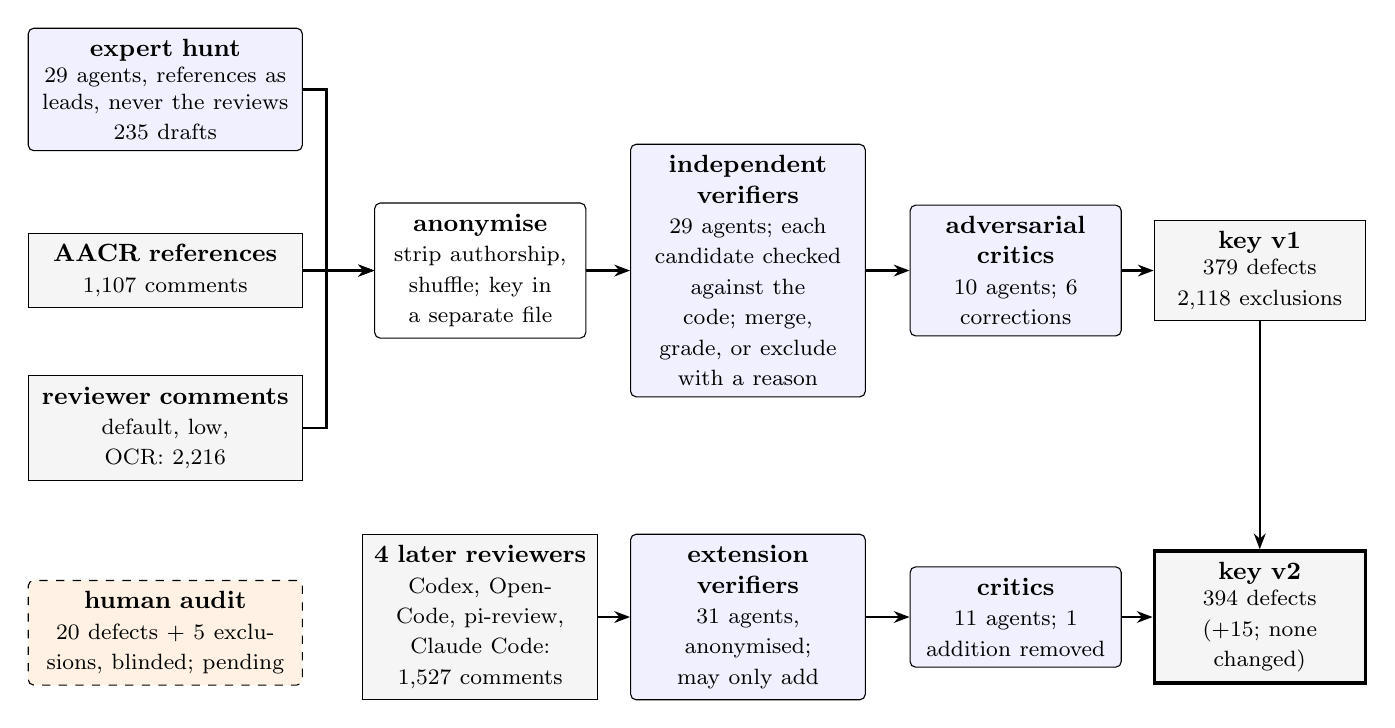
\begin{tikzpicture}
  \node[agent, text width=3.2cm] (hunt) at (-0.3,2.3) {\textbf{expert hunt}\\ \footnotesize 29 agents, references as leads, never the reviews\\ 235 drafts};
  \node[data, text width=3.2cm] (refs) at (-0.3,0) {\textbf{AACR references}\\ \footnotesize 1{,}107 comments};
  \node[data, text width=3.2cm] (com) at (-0.3,-2.0) {\textbf{reviewer comments}\\ \footnotesize default, low, OCR: 2{,}216};
  \node[box, text width=2.4cm] (anon) at (3.7,0) {\textbf{anonymise}\\ \footnotesize strip authorship, shuffle; key in a separate file};
  \node[agent, text width=2.7cm] (ver) at (7.1,0) {\textbf{independent verifiers}\\ \footnotesize 29 agents; each candidate checked against the code; merge, grade, or exclude with a reason};
  \node[agent, text width=2.4cm] (crit) at (10.5,0) {\textbf{adversarial critics}\\ \footnotesize 10 agents; 6 corrections};
  \node[data, text width=2.4cm] (v1) at (13.6,0) {\textbf{key v1}\\ \footnotesize 379 defects\\ 2{,}118 exclusions};
  \draw[flow] (hunt.east) -- ++(0.3,0) |- (anon.west);
  \draw[flow] (refs) -- (anon);
  \draw[flow] (com.east) -- ++(0.3,0) |- (anon.west);
  \draw[flow] (anon) -- (ver);
  \draw[flow] (ver) -- (crit);
  \draw[flow] (crit) -- (v1);

  \node[data, text width=2.7cm] (com2) at (3.7,-4.4) {\textbf{4 later reviewers}\\ \footnotesize Codex, OpenCode, pi-review, Claude Code: 1{,}527 comments};
  \node[agent, text width=2.7cm] (ext) at (7.1,-4.4) {\textbf{extension verifiers}\\ \footnotesize 31 agents, anonymised; may only add};
  \node[agent, text width=2.4cm] (crit2) at (10.5,-4.4) {\textbf{critics}\\ \footnotesize 11 agents; 1 addition removed};
  \node[data, text width=2.4cm, very thick] (v2) at (13.6,-4.4) {\textbf{key v2}\\ \footnotesize 394 defects\\ (+15; none changed)};
  \draw[flow] (com2) -- (ext);
  \draw[flow] (ext) -- (crit2);
  \draw[flow] (crit2) -- (v2);
  \draw[flow] (v1) -- (v2);

  \node[human, dashed, text width=3.2cm] (aud) at (-0.3,-4.6) {\textbf{human audit}\\ \footnotesize 20 defects + 5 exclusions, blinded; pending};
\end{tikzpicture}}
\caption{How the answer key for the 145 new PRs was built. Every candidate
--- from the hunt, the dataset's references and the reviewers' comments ---
reaches the verifiers without its author. The original 40 PRs were built
the same way a day earlier (Section~\ref{sec:gt40}). The comments of the
final comparison's gpt-6.1-sol runs were never candidates
(Section~\ref{sec:outofpool}).}
\label{fig:gtpipeline}
\end{figure}


\begin{enumerate}
  \item \textbf{Code extraction} in a network-less container: per PR the
  diff, base and head versions of every changed file, a bare git store
  for reading the whole repository at head, the PR metadata, and the AACR
  references with model names stripped.
  \item \textbf{Expert hunt}: 29 Claude agents, about five PRs each.
  Output: 235 draft defects (46 high); 134 references judged real, 973
  rejected.
  \item \textbf{First reviews}: \qcr{} default, \qcr{} low and
  open-code-review ran on rest145.
  \item \textbf{Independent verification}: 29 Claude agents, about five
  PRs each. Every candidate --- the hunt's drafts, all 1{,}107
  references, and all 2{,}216 reviewer comments (default 978, low 663,
  OCR 580) --- was checked against the code. Reviewer comments were
  anonymised and shuffled; the key mapping them to reviewers sat in a
  separate file the agents were told never to open. Duplicates were
  merged, severities graded, and every rejection recorded with a
  one-sentence restatement of the claim first (so the judge can later
  recognise it in a review). 2{,}118 exclusions.
  \item \textbf{Adversarial critic}: 10 agents, one per about 15 PRs,
  spot-checked every high-severity defect, a sample of other defects,
  exclusions, merges and grades against the code and fixed the truth in
  place: 6 corrections.
  \item \textbf{Repair}: one PR's candidate list was renumbered after
  verification; it was re-verified by one agent so every provenance id is
  correct.
  \item \textbf{Assembly} into \code{defects/rest145.json} v1:
  \textbf{379 defects} (55 high / 113 medium / 211 low), validated with
  the judge's own parser.
\end{enumerate}

\emph{Provenance audit.} Of the 2{,}118 exclusions, 1{,}150 were
reviewer comments (default 550, low 345, OCR 255), 965 were AACR
references and 3 were hunt drafts. Of the 379 v1 defects, 138 were not in
the hunt: 8 high, 30 medium and 100 low (129 raised only by reviewer
comments, 9 by a reference and reviewer comments). Against the key's
55/113/211, the hunt alone missed 15\% of the high-severity defects and
47\% of the low ones.\footnote{Computed from
\code{rest145-code/<id>/truth.json}, \code{candidates-key.json} and
\code{hunt.json} in the analysis tree, 2026-09-29.}
Where both raised a defect, the verifier mostly kept the hunt's grade.
Each of the 241 hunt-flagged defects was matched to its hunt draft by
site overlap and text similarity; on the 234 confident matches the grade
was unchanged for 220 (94.0\%, $\kappa = 0.91$), raised for 8 (5
low$\to$medium, 3 medium$\to$high) and lowered for 6 (3 medium$\to$low,
2 high$\to$low, 1 high$\to$medium). Eight hunt drafts were split into
more than one defect.\footnote{Computed from \code{hunt.json} and
\code{truth.json} per PR (matching script \code{wp-data/prov.py}),
2026-09-29. The seven weakest matches were left out because some of them
paired a defect with the wrong draft; with them included the figures are
92.9\% and $\kappa = 0.89$.}

\subsection{Extension with four more reviewers (v2)}

After Codex CLI, OpenCode, pi-review and Claude Code had run, every one of
their comments on all 185 PRs (1{,}527 candidates: OpenCode 557, pi-review
395, Codex 390, Claude Code 185 whole review texts) was anonymised,
shuffled by a hash of the comment text, and checked against the code and
the current truth by 31 verifier agents. A Claude Code review is prose, so
each whole review is one candidate whose claims are checked one by one
(which is why the outcomes below sum to more than 1{,}527). Results: 931
matched an existing defect, 691 excluded with reasons (572 of them on
rest145, now in \code{defects/rest145.json}), 16 added. Eleven critics
checked every addition and removed one (4 critic corrections in total).
Net \textbf{+15 defects}: rest145 v2 has \textbf{394 defects} (56 high /
114 medium / 224 low). The assembly script refused to write if any
existing defect was dropped or changed, and the version number was bumped
so verdicts from the two versions never mix. Every reviewer in both
studies is judged on v2.

The same pass over the original 40 PRs added no defect, so their files and
versions were not changed; their new exclusions are kept only in the
analysis folder.

\emph{Why extend rather than rebuild.} Rebuilding the key from scratch with
all seven reviewers in the pool would have given every tool an equal-sized
seat, at the cost of redoing a verification that had already been
critic-checked. We chose to extend, and to measure the resulting
seeding bias directly (Section~\ref{sec:independent-sol}). The small yield
(15 new defects from 1{,}527 comments) is evidence that the pool was close
to saturated; it is not proof.
The saturation curve says the same. On rest145, where every comment can
be traced to its reviewer, start from the 250 defects that the hunt or an
AACR reference raised and add the seven reviewers one at a time. Averaged
over all 5{,}040 orders, the reviewers add 69.1, 30.1, 17.3, 11.0, 7.4,
5.2 and 3.7 defects, so the seventh reviewer contributes under 1\% of the
394. The average marginal contribution per reviewer is: default 42.6,
Claude Code 21.9, low 21.7, OCR 19.6, pi-review 14.2, Codex CLI 12.1,
OpenCode 11.8. Without the hunt and the references, the reviewers' union
grows 237, 303, 336, 356, 368, 377, 382.\footnote{Computed from
\code{provenance} in \code{truth-ext.json} and the two candidate keys per
PR (\code{wp-data/prov.py}), 2026-09-29.}
The curve flattens for this pool of reviewers only. It says nothing about
defects that none of them would raise.

\subsection{The original 40 PRs}
\label{sec:gt40}

The original 40 were built earlier (2026-09-26/27) with the same shape:
a blind hunt per PR, then a consolidator checking the hunt, the AACR
references (with hand labels) and every anonymised comment from our runs
and OCR's, then a critic per set (12 corrections). Version 2 of smoke10,
dev10 and holdout10 added the judge's ``new defect'' candidates after
checking them against the code: 44 candidates from 12 judged runs, 1
added, 2 restated existing defects, 41 rejected. fresh10 (v1) was built
from a blind hunt and the comments of both of \emph{our} arms plus the
references; \textbf{OCR's comments were not candidates for fresh10}, so
OCR may be under-credited on those 10 PRs.

\subsection{The final key}

\begin{table}[t]
  \centering
  \caption{The answer key. Counts from FULL-BENCHMARK.md.}
  \label{tab:gt}
  \begin{tabular}{lll}
    \toprule
     & Original 40 & New 145 \\
    \midrule
    Defects & 126 (34 high / 31 medium / 61 low) & 394 (56 high / 114 medium / 224 low) \\
    Version & smoke10, dev10, holdout10 v2; fresh10 v1 & v2 (v1: 379 defects) \\
    Built & 2026-09-26/27 & v1 2026-09-28; v2 extension 2026-09-28 \\
    \bottomrule
  \end{tabular}
\end{table}

In total: \textbf{520 defects (90 high / 145 medium / 285 low)} over 185
PRs (Table~\ref{tab:gt}). Descriptive counts from the committed
files:\footnote{Computed from \code{bench/aacr/defects/*.json},
re-verified 2026-09-28.} 26 PRs have no defect; the median PR has 2 and
the maximum is 17; the original 40 average 3.15 defects per PR and
rest145 2.72. By kind: bug 229, maintainability 72, incomplete-fix 57,
build 42, contract 29, data 23, compat 21, security 13, resource 12,
concurrency 11, performance 9, other 2 (one behaviour regression, one
logic).

Three CI-gate defects (a lint rule, stale generated SQL, a clippy failure)
carry a \code{benchmark\_limitation} note: a read-only review can find
them only by knowing the repository's CI. They are counted in every table
and reported apart.

\paragraph{Provenance on rest145 (v1).} Table~\ref{tab:prov} shows where
the 379 v1 defects came from. A defect may have several sources.

\begin{table}[t]
  \centering
  \caption{Sources of the 379 rest145 v1 defects.}
  \label{tab:prov}
  \begin{tabular}{lrr}
    \toprule
    Source & Defects it raised & Only this source \\
    \midrule
    \qcr{} default's comments & 334 & 29 \\
    \qcr{} low's comments & 269 & 3 \\
    Expert hunt & 241 & 12 \\
    open-code-review's comments & 230 & 4 \\
    AACR references & 115 & --- \\
    \bottomrule
  \end{tabular}
\end{table}

\qcr{} default is the largest single contributor: 334 of 379 defects (88\%)
and 29 that no other source raised. This is the main reason for the
independent-source check in Section~\ref{sec:independent-sol}. Of each
first-pass reviewer's own comments, 44\% (default, 978 comments), 48\%
(low, 663) and 56\% (OCR, 580) map onto a real defect; the rest are
maintainability notes, questions and nits, whose truth is graded
separately (``comments correct''). Default's large contribution to the
pool is partly a matter of volume: it posts the most comments, and the
lowest share of them map onto a defect (Section~\ref{sec:disagree}).

\subsection{Who built the key}

Claude agents (Claude Code subagents on Opus 5.5) built and critiqued the
key throughout. That family is independent of the OpenAI-based reviewers
but is the same family as the Claude Code reviewer and the second judge.
The same assistant that designed \qcr{}'s benchmark levers also
orchestrated the key and wrote the judge prompt. \textbf{No human has
checked the 394 rest145 defects.}
\NEEDEXP{Human audit of the key, scope decided: one engineer audits 20 defects
on Python PRs and 5 exclusions, blinded; the audit sheet, with full context per item, is ready and
awaits the auditor. Publish the
agreement rate here and correct the key where the audit overturns it.
This is the single most important missing experiment.}

% =====================================================================
\section{Judging}
\label{sec:judging}

\subsection{The defect judge}

One judge session per PR, with read-only access to the repository
checked out at the PR head, reads:
\begin{itemize}
  \item the PR's defect list, each with its statement, sites and ``counts
  if'' notes;
  \item the claims already checked and rejected for this PR, each with
  its reason (capped at 600 characters each, 14{,}000 in total);
  \item the review as the author would receive it: verdict, body (capped
  at 12{,}000 characters) and every comment with path and line.
\end{itemize}

It returns, in strict JSON checked by a parser:
\begin{itemize}
  \item per defect: \emph{found} (some comment or the body identifies
  this defect with its essential point right), \emph{partial} (points at
  the problem or its site but with a wrong or missing mechanism or
  consequence), or \emph{missed};
  \item per comment: which defect it finds (or none), and a grade:
  correct-valuable, correct-minor, partly-correct, incorrect, or
  unverifiable.
\end{itemize}

The full prompt is reproduced in \code{docs/PROMPTS.md} \S2 and summarised
in Appendix~\ref{app:prompts}.

\paragraph{Design decisions in the judge.}
\begin{itemize}
  \item \emph{Location-agnostic.} A defect counts as found wherever in the
  review it is said --- cause site, symptom site, another line, or the
  body. \emph{Rejected:} a line gate like AACR's, which drops the right
  finding two lines away before any judge sees it.
  \item \emph{Substance over form.} Wording, tone, tags and exact line
  numbers do not matter. The ``counts if'' notes, written by the verifier,
  state the essential point, so a vague comment near the right line does
  not count.
  \item \emph{Partial credit of one half.} \emph{Rejected:} binary scoring,
  which either credits a comment whose mechanism would make the author fix
  the wrong thing, or gives it nothing although it pointed at the site.
  Partial credit does not drive the ranking: with partials counted as
  zero, recall under the primary judge is default 83.7\%, low 65.4\%,
  Claude Code 61.5\%, pi-review 55.4\%, OCR 55.2\%, OpenCode 47.5\%, Codex
  CLI 47.3\% --- each within one point of its headline figure, in the same
  order.\footnote{Computed from the primary judge's verdict files
  (\code{judge/v<ver>-gpt-6-sol-high/*.r1.json} in the runs listed in
  \code{FULL-BENCHMARK.md}, first judged run per PR as in
  \code{compare.py}), 2026-09-28. Under the second judge the found-only
  figures are 84.2, 65.6, 60.6, 54.2, 55.4, 47.3 and 46.9\% in the same
  reviewer order.}
  \item \emph{The judge sees the rejected claims.} A comment repeating a
  rejected claim is graded against its recorded reason instead of being
  re-adjudicated from scratch. \emph{Rejected:} hiding exclusions, which
  lets the judge re-accept a plausible claim the verifier already refuted
  with code. This makes the judge stricter for every tool equally; since
  the exclusions were written from the tools' own comments, it also cuts
  both ways.
  \item \emph{Errors are not misses.} A failed judgement is stored as an
  error file; \code{compare.py} counts it as ``not judged'' and prints the
  row as incomplete. Every final row is 185/185.
\end{itemize}

\subsection{Metrics}

\begin{itemize}
  \item \textbf{Problems found}: found $+ \tfrac12\,$partial, summed over
  defects; \textbf{recall} is that over the number of defects.
  \item \textbf{Found by severity}: the same, per severity class.
  \item \textbf{Weighted recall}: severity weights high 3, medium 2, low 1.
  \item \textbf{Comments correct}: the share of the review's comments the
  judge grades correct-valuable or correct-minor.
\end{itemize}

``Comments correct'' merges a reviewer that posts many true minor notes
with one that posts few valuable ones, so every comparison also reports
the full grade breakdown (Tables~\ref{tab:grades}
and~\ref{tab:grades-sol}).

\subsection{Two judges from different model families}

\emph{Choice.} The primary judge is \code{gpt-6-sol} at high reasoning.
The same prompt, byte for byte, with the same inputs and the same parser,
was run a second time on \code{claude-opus-5-5} over all 1{,}295 reviews
(7 reviewers $\times$ 185 PRs). Verdicts are stored side by side.

\emph{Why.} The primary judge shares a model family with six of the seven
reviewers, including ours. A judge may prefer its own family's
outputs~\cite{panickssery2024,zheng2023}.
\emph{Rejected:} a single judge with that caveat stated. \emph{Rejected:}
a Claude-only judge, which would share a family with the key builder and
with Claude Code.

\paragraph{Agreement.}
\begin{itemize}
  \item \textbf{Per defect}: the two judges gave the same verdict (found,
  partial, missed) on \textbf{3{,}593 of 3{,}640} reviewer--defect pairs
  (98.7\%); on high-severity defects, 628 of 630.
  \item \textbf{Problems found}: every reviewer is within $\pm3$ defects;
  recall is identical after rounding for all seven.
  \item \textbf{Comments correct}: differs by up to 5 points. The largest
  gaps are Claude Code (81\% under GPT, 86\% under Opus) and OCR (73\% vs
  77\%).
\end{itemize}

The pair counts are 7 reviewers $\times$ 520 defects (3{,}640) and
7 $\times$ 90 high-severity defects (630). Raw agreement flatters a
three-way verdict whose classes are unbalanced, so we also report chance
correction: Cohen's $\kappa = 0.974$~\cite{cohen1960} on found/partial/missed, and
$\kappa = 0.986$ when partial and found are merged (99.3\% raw). Of the 47
disagreements, 45 involve a \emph{partial} on one side; only 2 are
found-vs-missed.\footnote{Computed from the two judges' verdict files
(\code{judge/v<ver>-gpt-6-sol-high/} and \code{judge/v<ver>-claude-opus-5-5/})
for the runs in \code{FULL-BENCHMARK.md}, 2026-09-28.}

Per comment the judges agree less: the same five-way grade on 3{,}972 of
4{,}455 comments (89.2\%), and the same correct/not-correct split on
91--95\% of each reviewer's comments. The largest movements are
partly-correct graded incorrect (99) or correct-valuable (91) by the
second judge, and correct-minor graded incorrect (82). This is where the
up-to-5-point differences in ``comments correct'' come from.
\emph{Judge self-consistency.} We re-ran the primary judge once, on the
same reviews, for 30 random PRs $\times$ all 7 reviewers (210 reviews,
637 reviewer--defect pairs, 742 comments). It gave the same defect
verdict on 99.7\% of pairs ($\kappa = 0.994$). Both disagreements
involve a \emph{partial}, and no verdict flipped between found and
missed. On the same sample the two judges agree on 99.2\% ($\kappa =
0.984$), so the difference between the judges is barely larger than the
primary judge's own run-to-run noise. Comment grades are noisier within
one judge too: the same five-way grade on 92.2\% ($\kappa = 0.87$) and
the same correct/not-correct split on 93.5\%, against 88.4\% and 90.6\%
between the judges on this sample. So about two-thirds of the
per-comment disagreement between the judges (7.8 of 11.6 points) is at the
level of the primary judge's disagreement with itself.\footnote{Computed from
\code{judge/wpself-gpt-6-sol-high/} (the re-run, a separate label; seed
20260929) against the published \code{judge/v<ver>-gpt-6-sol-high/} and
\code{judge/v<ver>-claude-opus-5-5/} verdicts (\code{wp-data/selfcons.py}),
2026-09-29. One round, 596 model calls, \$7.18 at list price.}

\paragraph{Why the final comparison has one judge.}
\label{sec:judgestab}
Two measurements say the grading is stable: a judge from another model
family reproduces the primary judge's verdicts almost exactly (98.7\%,
$\kappa = 0.97$, recall identical after rounding for all seven
reviewers), and the primary judge reproduces itself on a re-run (99.7\%,
$\kappa = 0.99$). The final comparison's reviews (Section~\ref{sec:results})
were therefore graded by the primary judge only. What that leaves
unchecked is the one effect the second judge was there to catch: a
preference of the judge's model family for reviews written by the same
family. The final OpenAI-based reviewers run on gpt-6.1-sol, the same
family as the primary judge; in the earlier study the only visible
same-family effect was on comments correct (the Claude judge was 5 points
kinder to Claude Code), not on recall.

\paragraph{What the agreement proves, and what it does not.} It shows that
the \emph{grading} --- whether a given review finds a given defect and
whether a comment is true --- is not an artefact of one model family or of
one model's reading of the prompt. A preference of either family for its
own reviewers would appear as disagreement, and there is almost none.
A bias both judges share --- for instance one induced by the common judge
prompt or by the ``counts if'' notes, both written by the key builder ---
would not appear as disagreement, which is why a re-judge with an
independently written prompt is listed below. The
one visible same-family effect is on accuracy, not recall: the Claude
judge is kinder to Claude Code's comments (81\% $\to$ 86\%), and Claude
Code's recall does not move (62\% under both).

It does \emph{not} validate the answer key. Both judges score against the
same 520 defects, built by one pipeline, with one prompt. Whether the key
is complete and correct rests on the verification pipeline
(Section~\ref{sec:gt}), the independent-source check
(Section~\ref{sec:independent-sol}), and the human audit we have not yet done.
A third judge from a family that matches neither gpt-6-sol nor Claude,
and a re-judge with an independently written judge prompt, are not done
(Section~\ref{sec:future}).

\paragraph{Operational note.} The Opus judge ran into the organisation's
rate limit for \code{claude-opus-5-5} (50 requests per minute; about 1.7
API calls per judgement). The first pass produced HTTP 429 error files;
the queue was stopped, resumed at lower parallelism, and a final resume
pass at parallelism 1 re-ran every remaining error. Final state: 0 errors
in 1{,}295 Opus judgements. The GPT judge left 2 error files, retried to 0.

\subsection{The AACR metric as we ran it}

The harness's evaluation stage ran unmodified at a pinned commit
(\code{68a5697}), \code{all} variant, 3 rounds averaged, line gate
$k=1$. Its judge prompt was answered by \code{gpt-6-sol} at low reasoning
through a local OpenAI-compatible shim, not by the paper's
\code{Qwen3-235B-A22B-Instruct-2507}~\cite{aacrbench}.
The shim makes one \code{pi -p} call per request and does not pass on the
harness's sampling parameters (temperature, top\_p), so those are the
model's defaults, not the harness's.
Evaluation was sharded by PR and merged with the harness's own summary
functions; on a copy of a finished run, sharded and unsharded results were
identical per round, average and PR.

\emph{Consequence.} Our AACR table is comparable across our own rows, not
with the published leaderboard.
\TODO{State why the paper's judge was not used (access, cost, or
endpoint). The README describes how to point the shim at Qwen3 through an
OpenAI-compatible endpoint.}
Two checks would place these numbers against the public leaderboard and
are not done: re-scoring all seven reviewers with the paper's judge
(\code{Qwen3-235B-A22B-Instruct-2507}), together with a re-run of a published leaderboard baseline
(open-code-review 1.3.1 with GPT-5.5) under both judges; and scoring the AACR metric under a
second judge family, as we did for the defect judge. The AACR judge is
noisy (the same pair was judged yes/yes/no across three calls in
testing), which is why three rounds are averaged.

% =====================================================================
\section{Reviewers and setup}
\label{sec:setup}

\begin{table}[t]
  \centering
  \small
  \caption{The eight reviewers of the final comparison, in the
  configuration Section~\ref{sec:bestshot} chose: pi-review~\cite{pireview}
  on pi~\cite{pi}, Claude Code~\cite{claudecode},
  open-code-review~\cite{ocr}, Codex CLI~\cite{codex},
  OpenCode~\cite{opencode} and PR-Agent~\cite{pragent}; the three harness
  runners are AACR-Bench's own~\cite{aacrrepo}. Versions are pinned by
  sha256/sha512. The earlier gpt-6-sol study's configurations are listed
  with Table~\ref{tab:bestshot}.}
  \label{tab:reviewers}
  \begin{tabularx}{\textwidth}{>{\raggedright\arraybackslash}p{2.7cm} >{\raggedright\arraybackslash}p{2.9cm} X}
    \toprule
    Reviewer & Model / effort & How it runs \\
    \midrule
    \qcr{} default & gpt-6.1-sol; lenses medium, validator and risk passes high &
      Production round with \textsc{benchmark mode}; preset \code{default}:
      every benchmark-driven lever, code-quality lenses, demoting
      validator, strict nits. Reads the PR title and body, as in production. \\
    \qcr{} low & gpt-6.1-sol, every role low & Same harness, preset \code{low} (lean plan). \\
    pi-review 0.18.0 (pi 0.99.1) & gpt-6.1-sol, thinking high & Its
      \code{code-experts} panel: three isolated read-only reviewers
      (correctness, security, testing), clustered, quorum two, singletons
      kept as advisories; diff attached as a file. \\
    Claude Code 2.1.283 & Claude Opus 5.5, session default & The
      harness's \code{reviewers/claude.py} (\code{/code-review base...head});
      findings parsed from its prose answer. \\
    open-code-review 1.3.1 & gpt-6.1-sol, effort high & Exactly as the
      harness's \code{reviewers/ocr.py}; model calls through a loopback bridge. \\
    Codex CLI 0.159.2 & gpt-6.1-sol, effort high & The harness's
      \code{reviewers/codex.py}: \code{codex exec review}, its prompt and
      MCP findings server; ChatGPT login. \\
    OpenCode 1.18.33 & gpt-6.1-sol, variant medium & Native ChatGPT
      provider, built-in \code{review} command (\code{subtask: true}) with the
      Codex runner's findings fragment, plus the PR title and body. \\
    PR-Agent 0.46.0 & gpt-6.1-sol, medium & Shipped defaults:
      \code{/describe}, \code{/review}, \code{/improve} on a local git
      provider, with the PR title and body. \\
    \bottomrule
  \end{tabularx}
\end{table}

\subsection{\qcr{} in brief}

\qcr{} is the authors' own reviewer. It runs one main session per PR,
which launches about eleven independent lens passes chosen from the diff
(a baseline, tests, a per-file sweep, code-quality lenses and
content-triggered sub-lenses) and then a validator that re-derives each
candidate finding from the code before one review is posted. Its
\code{default} and \code{low} presets differ only in reasoning effort. Its
design, the levers it gained while we built this benchmark, and its
base-model study are described in a companion report~\cite{qcrreport}.

\subsection{Deviations per third-party tool, and their direction}

In the final comparison:
\begin{itemize}
  \item \textbf{Codex CLI}: web search disabled could disfavour it, but no
  arm could search. Version 0.159.2 instead of the harness-era 0.158.0,
  because the ChatGPT backend refuses 0.158.0's requests for
  gpt-6.1-sol. Otherwise neutral.
  \item \textbf{OpenCode}: no harness runner exists; built in the Codex
  runner's shape on OpenCode's own provider and review command. gpt-6.1-sol
  is declared as a custom model on that provider, because 1.18.33's
  catalogue predates it. It reads the PR title and body, which the harness
  never passes.
  \item \textbf{pi-review}: its panel at its shipped reasoning level, on
  pi 0.99.1 with pi's new built-in extensions switched off. It does not
  read the PR text; on gpt-6-sol the PR text was worth 1.5 defects to it
  on 40 PRs (Table~\ref{tab:bestshot}), so this mildly \emph{disfavours}
  it.
  \item \textbf{Claude Code}: see below. Parsing errors mainly lower its
  AACR numbers and may move its comments-correct share either way. Its
  read-only \code{git} commands were denied on 46 of 185 PRs, which may
  disfavour it; it was not re-run at a higher review level: its session default
  (medium) matches \qcr{}'s medium lenses, and we kept it there.
  \item \textbf{open-code-review}: runs exactly as the harness's runner, at
  effort high set at our model bridge (1.3.1 has no effort flag).
  \item \textbf{PR-Agent}: run on a local git provider rather than
  GitHub, with its shipped defaults, including a 32k-token prompt budget
  that pruned 4 of the 40 selection diffs, as it would for any user.
\end{itemize}
In the earlier gpt-6-sol study three deviations disfavoured a tool, and
Section~\ref{sec:bestshot} measured them: pi-review at its default high
effort ($+10$ points) and with its panel ($+16$), OpenCode on its native
provider ($+7$, at less than half the cost), and Codex CLI and
open-code-review at high effort ($+12$ and $+2$). OpenCode's
\code{subtask: false} there removed a duplicate-reporting penalty and so
favoured it.

\subsection{Claude Code's prose parser}

In Claude Code 2.1.283, \code{/code-review} is a bundled skill~\cite{claudecode}.
It ignores the harness's appended system prompt and its findings tool,
and answers in markdown prose. The harness therefore records zero
structured findings (the logs say \code{0 finding(s)} for 182 of the 185
logged cases). We wrote a deterministic parser
(\code{src/bench/claudeprose.ts}, 12 golden fixtures, rules read off 150
real outputs) that reads \code{path:line} findings out of the prose; it
was applied after the fact without re-reviewing.

\emph{Rejected: re-prompting Claude Code for structured output.} That
would have changed the tool as shipped. \emph{Rejected: scoring it as
zero.} That would have measured the harness's integration, not the
review.

Effect by metric: the defect judge reads the full prose as the review
body as well as the parsed comments, so defect recall depends little on
the parser. ``Comments correct'' grades the parsed comments. The AACR
metric scores only parsed comments, so a finding without a line number is
lost there.
\emph{Parser coverage.} The parser read 174 of the 185 reviews; the other
11 came back through the harness's findings tool (3 with findings, 8
empty). From the 174 it extracted 402 located findings, a mean of 2.3 per
review (median 2, maximum 9; 29 reviews with none, mostly ``I found no
bugs''). It set aside 7 unlocated items in 3 reviews, 7 located items
under ``not a finding'' lead-ins and 4 recap items. We then hand-checked
20 random reviews against their \code{review.md}. They contain 45
findings. The parser extracted 44 of them, each with the right path and
line, and extracted nothing that was not a finding. The one miss names a
file but no line, which the rules leave out by design. Informally, that
is precision 100\% and recall 98\% on the sample.\footnote{Computed from
\code{bench.claude\_prose\_parsed} in each result file and a reading of
20 sampled reviews (seed 20260929), 2026-09-29.}

\subsection{Execution}

Arms ran through a machine-wide scheduler with at most 10 concurrent
reviews per model login. In the earlier study the \qcr{} arms ran 10 PRs at
a time; the single-pass tools ran one PR at a time per container and, on
rest145, in four parallel chunks. For Codex and OpenCode a serial run had
already reviewed 18 and 19 PRs; those were kept and the chunks covered the
rest. \code{compare.py} takes the first run with a judgement per PR, so no
PR is counted twice. The scheduler re-ran one \code{no-output} default
case and one failed OCR case. The final comparison's third-party and
\code{low} runs were launched fresh in two halves (the 40 selection PRs and
the other 145) and every case finished; the machine was kept awake with a
sleep inhibitor after an auto-suspend stalled one earlier run for five
hours.

\subsection{Cost accounting}

Costs are list-price equivalents, not bills.
\begin{itemize}
  \item gpt-6.1-sol arms (the final comparison): \$2 per million uncached
  input tokens, \$0.10 per million cached input tokens, \$10 per million
  output tokens; gpt-6-sol arms (the earlier study): the same with \$0.20
  per million cached tokens. For \qcr{} and pi-review these are pi's
  list prices, summed over the main session and every pass. Cached input is
  priced at the cached rate; two calls were recomputed by hand from raw
  counts and matched pi to the digit.
  \item Arms reporting OpenAI-style usage (OCR, OpenCode through the
  loopback bridge; Codex CLI natively): the cached count is subtracted
  from input and priced at the cached rate.
  \item Claude Code: its own reported \code{total\_cost\_usd}, an
  API-price equivalent at Anthropic's list price; its uncached column
  includes cache writes.
\end{itemize}
All OpenAI-model runs (every gpt-6-sol and gpt-6.1-sol arm, and the gpt-6-luna arm of the
companion report's base-model study~\cite{qcrreport}) went through a
ChatGPT subscription login; Claude Code and that study's Opus arm went
through the Anthropic API. What the
subscription runs would have cost on OpenAI's API is unknown, so every
OpenAI-model cost here is pi's list price, not a bill. The relative cost
of OCR, OpenCode and \qcr{} low depends on the cached-token rate, so a
published API price could reorder them.
\emph{Judge cost.} Judging the 1{,}295 reviews (7 reviewers $\times$ 185
PRs) once cost \$41.85 at list price with the primary defect judge. That
is 3{,}713 model calls, 13.4M uncached input, 16.2M cached input and 1.2M
output tokens, or \$0.035 per review. The second judge (Opus 5.5 at
\$4/\$20 per million input/output tokens, \$0.2 cache read, \$5 cache
write) cost \$54.16: 2{,}448 calls, 6.8M cache-write, 4.0M cache-read and
1.0M output tokens, or \$0.045 per review. The 96 reviews with neither
defects nor comments needed no call. Per reviewer, the primary judge cost
\$5.0--8.0 and the second \$6.6--10.3, with default the most expensive to
judge in both.\footnote{Computed from the assistant \code{message\_end}
usage in \code{judge/v<ver>-\{gpt-6-sol-high,claude-opus-5-5\}/}\allowbreak\code{<id>.r1.events.jsonl}
for the runs in \code{FULL-BENCHMARK.md} (\code{wp-data/cost.py}),
2026-09-29. Recomputing from the raw token counts at these rates matches
pi's own cost total to the cent.}
The AACR judge shim records no token usage, so its cost is an estimate.
With a $\pm1$ line gate, the seven reviewers' comments give 7{,}986
reference--comment pairs per round that reach the judge. A round makes at
most that many calls, since matching stops at the first semantic match,
so three rounds make at most 23{,}958. The prompt averages about 1{,}530
characters (about 425 tokens) and the answer is a word plus low-effort
reasoning, about 40 tokens. At gpt-6-sol rates that is about \$0.0013 a
call, or at most about \$30 for the three-round AACR table. The real
count is lower. A one-round re-score with the looser $\pm5$ gate made
3{,}227 calls, which bounds a $\pm1$ round from above, so the three-round
table costs about \$12 or less. The shim logs that survive record 10{,}752
calls (about \$13), and those include the extra variants some runs
scored.\footnote{Estimated from the harness's judge prompt
(\code{evaluation/judge.py}), the result files, the
\code{eval/judge-shim.log} of each run and the line-gate diagnostic's shim
logs (\code{wp-data/cost.py}), 2026-09-30.}

% =====================================================================
\section{Choosing each tool's configuration}
\label{sec:bestshot}

The earlier study (Section~\ref{sec:sol}) ran each third-party tool as
shipped, or as the AACR harness runs it. A fairness audit of those runs
(2026-09-30) read each tool's own documentation, shipped configuration
files and binaries, and every run's transcripts, and asked whether each
tool had been given its best shot. It found three that had not: pi-review
ran below its own default reasoning level and without its panel, OpenCode
ran through our compatibility bridge instead of its own provider, and no
tool but \qcr{} (and PR-Agent, below) was given the PR title and body.
This section measures each tool in the configurations its own
documentation ships or recommends, picks one per tool by a rule fixed in
advance, and measures what the pick itself is worth.
Figure~\ref{fig:protocol} shows the four steps.

\begin{figure}[t]
\centering
\resizebox{\textwidth}{!}{%
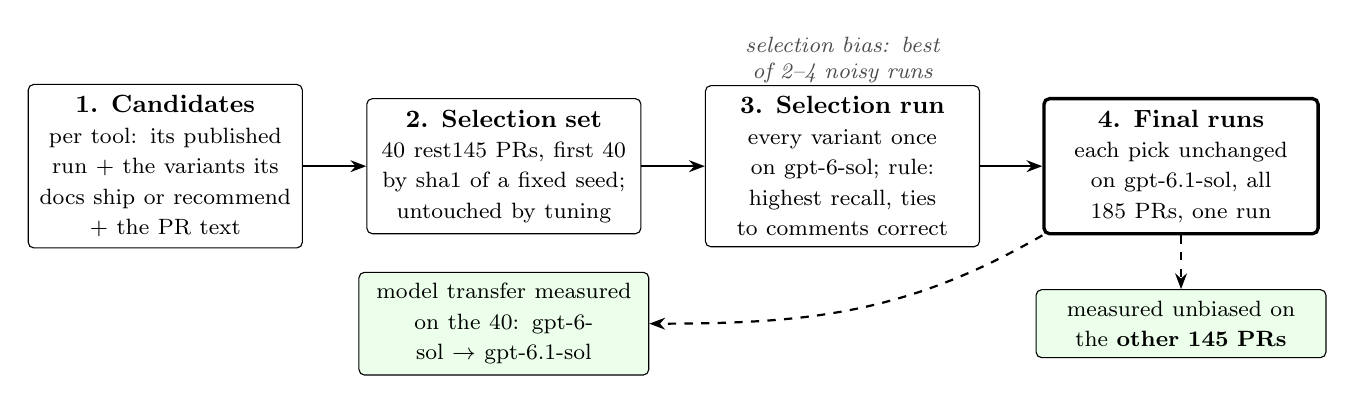
\begin{tikzpicture}
  \node[box, text width=3.2cm] (s1) at (0,0) {\textbf{1. Candidates}\\ \footnotesize per tool: its published run + the variants its docs ship or recommend + the PR text};
  \node[box, text width=3.2cm] (s2) at (4.3,0) {\textbf{2. Selection set}\\ \footnotesize 40 rest145 PRs, first 40 by sha1 of a fixed seed; untouched by tuning};
  \node[box, text width=3.2cm] (s3) at (8.6,0) {\textbf{3. Selection run}\\ \footnotesize every variant once on gpt-6-sol; rule: highest recall, ties to comments correct};
  \node[box, text width=3.2cm, very thick] (s4) at (12.9,0) {\textbf{4. Final runs}\\ \footnotesize each pick unchanged on gpt-6.1-sol, all 185 PRs, one run};
  \draw[flow] (s1) -- (s2); \draw[flow] (s2) -- (s3); \draw[flow] (s3) -- (s4);
  \node[note, text width=3.6cm] at (8.6,1.35) {selection bias: best of 2--4 noisy runs};
  \node[judge, text width=3.4cm] (u) at (12.9,-2.0) {\footnotesize measured unbiased on the \textbf{other 145 PRs}};
  \node[judge, text width=3.4cm] (t) at (4.3,-2.0) {\footnotesize model transfer measured on the 40: gpt-6-sol $\to$ gpt-6.1-sol};
  \draw[flow, dashed] (s4) -- (u);
  \draw[flow, dashed] (s4.south west) to[out=-150,in=0] (t.east);
\end{tikzpicture}}
\caption{The best-shot protocol. \qcr{} was not tuned in steps 1--3: its
\code{default} preset is its row, with \code{low} as a second, cheaper
point. Claude Code stayed at its published configuration, whose medium
level matches \qcr{}'s medium lenses.}
\label{fig:protocol}
\end{figure}

\paragraph{The 40 PRs.} A seeded sample of rest145 (seed string
\code{fairness-2026-09-30}, sha1 order): 115 defects, 17 high, 33 medium,
65 low. None was used to tune \qcr{}. Every arm is 40/40 judged by the
primary judge; every configuration ran once.

\paragraph{The variants.} All on gpt-6-sol unless stated.
\begin{itemize}
  \item \textbf{pi-review 0.18.0}~\cite{pireview}: \code{-{}-thinking high}, its shipped
  \code{code} preset's default; high plus the PR text; and the
  \code{code-experts} panel (three reviewers for correctness, security and
  testing, quorum two, singletons kept as advisories) at high, which is
  what pi-review's \code{/rv} command runs by default in the pi
  host~\cite{pireview}.
  \item \textbf{Codex CLI 0.158.0}~\cite{codex}: reasoning effort high (its
  default for gpt-6-sol is medium); medium plus the PR text.
  \item \textbf{open-code-review 1.3.1}~\cite{ocr}: effort high at the model endpoint
  (1.3.1 has no effort flag); medium plus the PR text through
  \code{-{}-background}, which its own agent skill marks as
  recommended~\cite{ocr}.
  \item \textbf{OpenCode 1.18.33}~\cite{opencode}: its native ChatGPT provider (Responses
  API, reasoning carried across turns, prompt cache) with the built-in
  \code{review} command at its default \code{subtask: true} and
  \code{-{}-variant medium}; the same plus the PR text.
  \item \textbf{PR-Agent 0.46.0}~\cite{pragent}, new to the benchmark: its shipped
  defaults and full GitHub-App flow (\code{/describe}, \code{/review},
  \code{/improve}; at most 3 key issues and about 3 suggestions; a
  32k-token prompt budget that prunes 4 of the 40 diffs, as it would for any
  user), reading the PR title and body as it does on GitHub; on gpt-6-sol
  and on gpt-6.1-sol.
  \item \textbf{Claude Code} was not re-run. It stays at medium, its
  session default, to match \qcr{}'s medium lenses; its read-only
  \code{git} denials (46 of 185 PRs) remain a stated limitation.
\end{itemize}
``PR text'' is the PR title and body, passed through each tool's own channel
exactly as \qcr{} receives it.

\begin{table}[t]
  \centering
  \caption{Best-shot configurations, 40 PRs of rest145, 115 defects (17
  high), primary judge. One run per configuration. Bold: the best
  configuration found per tool. AACR columns: 360 references on these PRs, 3
  judge rounds averaged; the last column removes the 30 bot-derived
  references (a comment matching only a removed reference counts as
  unmatched).}
  \label{tab:bestshot}
  \resizebox{\textwidth}{!}{%
  \begin{tabular}{llrrrrrrrrr}
    \toprule
    Tool & Configuration & Found & Recall & High & Correct & \$/PR & Min & AACR R / P & AACR F1 & F1, bot refs out \\
    \midrule
    \qcr{} & default, as published & 98.5 & 86\% & 16 & 81\% & 2.11 & 9.5 & 11.0\% / 13.1\% & 12.0\% & 9.1\% \\
     & default, current build & \textbf{103} & \textbf{90\%} & \textbf{17} & 87\% & 2.12 & 9.7 & 11.0\% / 13.1\% & 12.0\% & 9.6\% \\
     & gpt-6.1-sol & 98 & 85\% & \textbf{17} & \textbf{94\%} & 1.64 & 10.9 & 11.4\% / 15.4\% & 13.1\% & 9.7\% \\
     & low preset & 77.5 & 67\% & 14 & 76\% & 0.93 & 4.7 & 8.3\% / 14.3\% & 10.5\% & 8.1\% \\
    \midrule
    Claude Code (Opus 5.5) & \textbf{as published (medium)} & 68.5 & 60\% & 14 & 77\% & 0.26 & 0.9 & 3.1\% / 12.2\% & 4.9\% & 4.8\% \\
    \midrule
    pi-review & as published (medium, 1 reviewer) & 59.5 & 52\% & 14 & 72\% & 0.11 & 1.0 & 3.9\% / 15.7\% & 6.2\% & 5.3\% \\
     & high & 71 & 62\% & 15 & 71\% & 0.17 & 3.0 & 5.5\% / 17.9\% & 8.4\% & 7.6\% \\
     & high + PR text & 72.5 & 63\% & 13 & 74\% & 0.18 & 3.0 & 5.2\% / 17.0\% & 7.9\% & 7.6\% \\
     & \textbf{3-reviewer panel, high} & 78 & 68\% & 15 & 78\% & 0.46 & 3.6 & 7.2\% / 16.0\% & 10.0\% & 9.3\% \\
    \midrule
    open-code-review & as published (medium) & 76 & 66\% & 13 & 73\% & 0.86 & 1.3 & 9.3\% / 17.3\% & 12.1\% & 8.5\% \\
     & \textbf{high} & 78 & 68\% & 14 & 76\% & 1.12 & 4.1 & 11.4\% / 17.9\% & 13.9\% & 10.0\% \\
     & medium + PR text & 78 & 68\% & 14 & 73\% & 0.87 & 2.7 & 9.1\% / 16.7\% & 11.8\% & 8.5\% \\
    \midrule
    OpenCode & as published (bridge) & 49 & 43\% & 12 & 57\% & 0.96 & 1.7 & 4.4\% / 14.4\% & 6.8\% & 5.4\% \\
     & native provider & 57 & 50\% & 13 & 67\% & 0.40 & 5.2 & 5.1\% / 11.3\% & 7.0\% & 5.8\% \\
     & \textbf{native + PR text} & 69.5 & 60\% & 13 & 66\% & 0.40 & 5.3 & 5.1\% / 10.9\% & 6.9\% & 6.6\% \\
    \midrule
    Codex CLI & as published (medium) & 51 & 44\% & 14 & 62\% & 0.19 & 1.7 & 2.8\% / 11.5\% & 4.5\% & 3.8\% \\
     & \textbf{high} & 64 & 56\% & 15 & 78\% & 0.24 & 4.8 & 4.1\% / 15.4\% & 6.4\% & 6.0\% \\
     & medium + PR text & 62.5 & 54\% & 13 & 70\% & 0.18 & 3.5 & 4.6\% / 17.7\% & 7.3\% & 6.9\% \\
    \midrule
    PR-Agent & gpt-6-sol & 34.5 & 30\% & 10 & 61\% & 0.10 & 3.2 & 6.8\% / 24.6\% & 10.6\% & 9.0\% \\
     & \textbf{gpt-6.1-sol} & 39.5 & 34\% & 11 & 63\% & 0.09 & 2.3 & 5.7\% / 23.8\% & 9.2\% & 7.5\% \\
    \bottomrule
  \end{tabular}}
\end{table}

\begin{figure}[t]
  \centering
  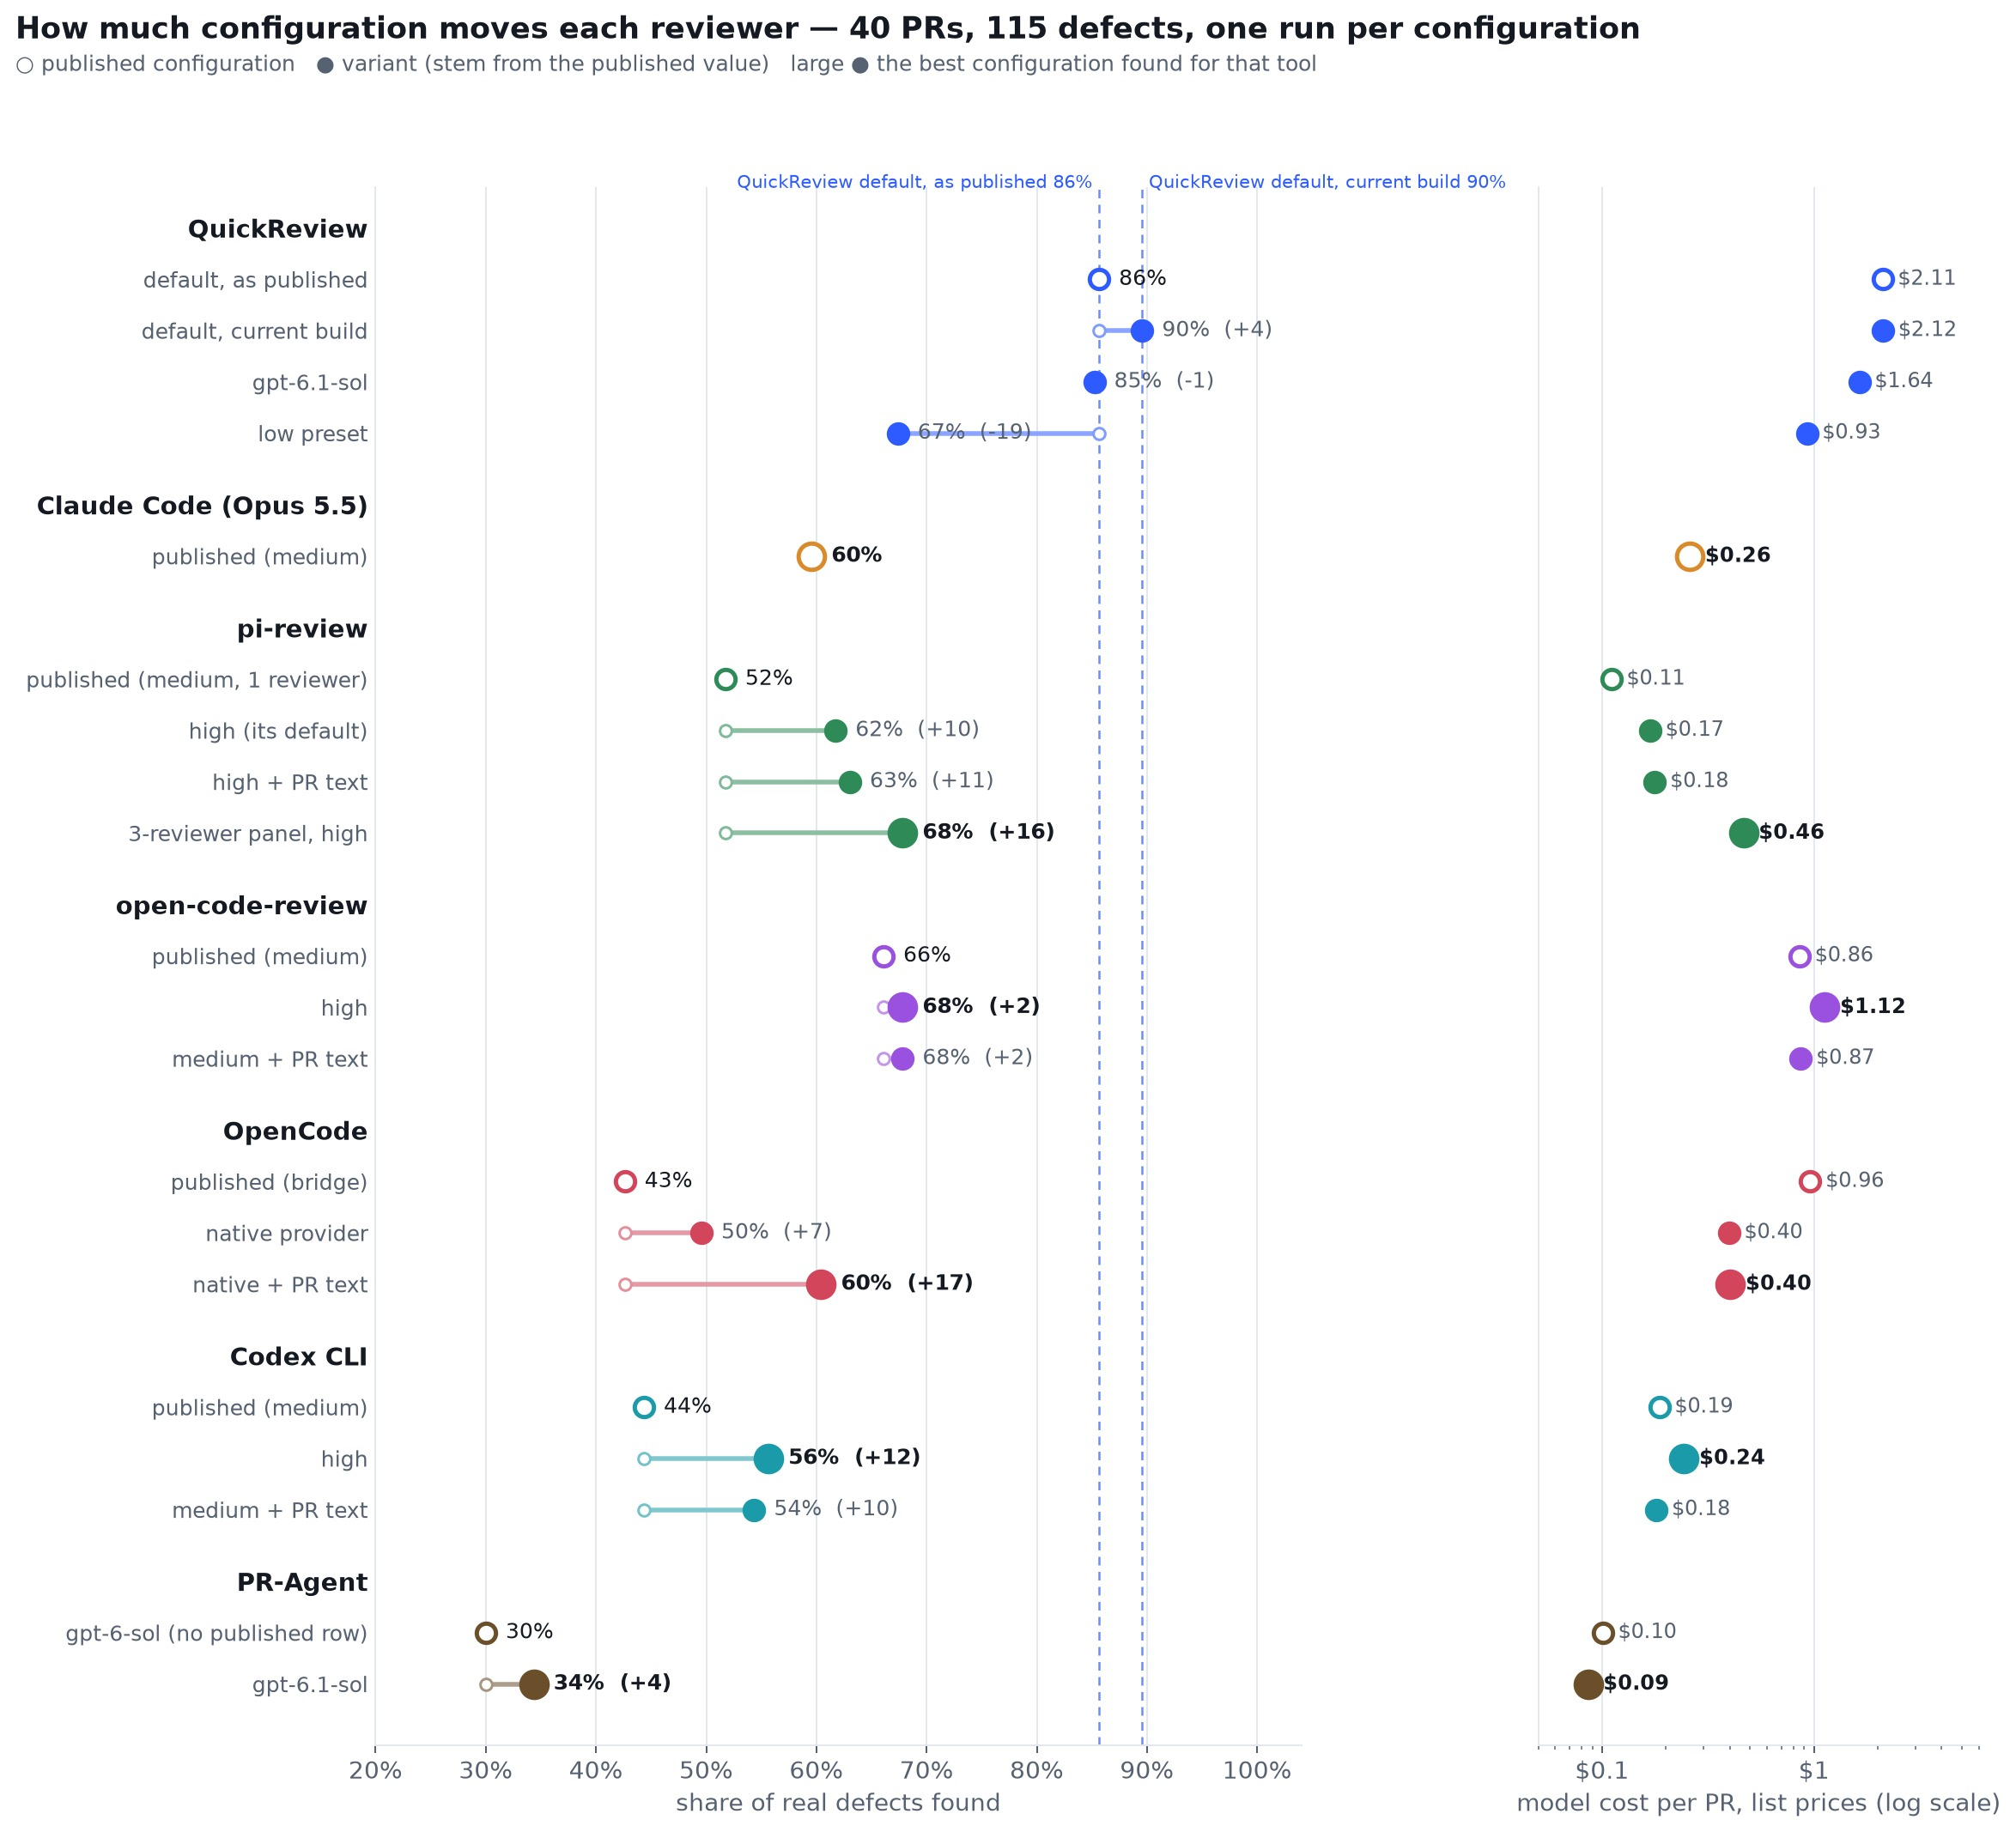
\includegraphics[width=\textwidth]{../charts/config-sensitivity.jpg}
  \caption{Configuration sensitivity on the 40 PRs. Left: share of real
  defects found per configuration; hollow markers are the published
  configurations, stems run from the published value to each variant, and
  the large marker is the best configuration found for that tool. Dashed
  lines: \qcr{} default as published (86\%) and on the current build
  (90\%). Right: model cost per PR at list prices, log scale.}
  \label{fig:configsens}
\end{figure}

\subsection{What configuration moved}

Table~\ref{tab:bestshot} and Figure~\ref{fig:configsens}.
\textbf{pi-review} gains 16 points (52\% to 68\%): its default reasoning
level alone gives 10, and the three-reviewer panel the rest, at 2.7 times
the cost of a single high reviewer (\$0.46 against \$0.17).
\textbf{OpenCode} gains 17 points (43\% to 60\%): the native provider gives
7 and cuts the cost from \$0.96 to \$0.40 per PR, because our bridge had lost
prompt caching and the published \$/PR was inflated; the PR text gives the
other 10. \textbf{Codex CLI} gains 12 points at high effort (44\% to 56\%)
and its comments-correct share rises from 62\% to 78\%, for \$0.05 more per
PR. \textbf{open-code-review}, already run as its harness runs it, moves
least: 2 points either way, with the best AACR F1 of any row at high effort
(13.9\%). \textbf{PR-Agent} finds 30--34\%, the fewest, with the highest
AACR precision (24--25\%), which is what a shipped cap of three key issues
produces. \qcr{} was not changed for this section: its current build finds
90\% on these 40 and gpt-6.1-sol 85\%.

Against the published configurations the gap on these 40 PRs was 20 points
(86\% against open-code-review's 66\%); against the best configurations we
found it is 18--22 points (86--90\% against 68\%), and on high-severity
defects 17 of 17 for the current build against at most 15. Giving every
tool its best shot moved the field up; it did not close the gap. These are
40 PRs and one run per configuration, and identical \qcr{} configurations
spread by about $\pm6$ points on samples of 26--30 PRs, so single-digit
differences between rows are not established.

\subsection{Selection rule and the picks}

The rule, fixed before any selection run: per tool, the configuration with
the highest defect recall on the 40 PRs; a tie goes to the higher share
of correct comments. The picks (bold in Table~\ref{tab:bestshot}):
pi-review's three-reviewer \code{code-experts} panel at thinking high
(68\%); open-code-review at effort high (68\%, tied on defects found with
medium plus PR text and ahead on comments correct, 76\% against 73\%);
OpenCode's native provider with the PR text (60\%); Codex CLI at effort
high (56\%); PR-Agent's shipped defaults on gpt-6.1-sol, the better of its
two models here (34\%); and Claude Code unchanged (60\%). These are the
best configurations \emph{we found} among those the tools' documentation
ships or recommends, not an exhaustive search. Not run, and said so:
Claude Code's \code{/code-review} at a higher level, pi-review at
\code{xhigh}, and repeated runs per configuration.

\subsection{Carrying the picks to gpt-6.1-sol}
\label{sec:transfer}

\qcr{}'s gpt-6.1-sol run already existed (the companion report~\cite{qcrreport}).
We then decided that every OpenAI-based contender should run on
gpt-6.1-sol, so that no comparison rests on a model difference between
them. The picks were re-run unchanged apart from the model, on the 40
selection PRs and the other 145 (2026-09-30 19:59 to 2026-10-01 00:16
UTC, after a two-PR smoke run per tool). Running each tool on the new
model took one change per tool, none of which alters its review
behaviour: pi-review moved to pi 0.99.1, the first release whose model
catalogue lists gpt-6.1-sol, with pi's new built-in extensions switched
off so it has the same tools as before; OpenCode's native provider got a
custom model entry for gpt-6.1-sol; Codex CLI moved from 0.158.0 to
0.159.2, because the ChatGPT backend refused 0.158.0's requests for the
new model; open-code-review and PR-Agent reach the model through our
loopback bridge, which now serves gpt-6.1-sol. Every image, version and
command is in \code{FULL-BENCHMARK.md} (``Exact commands'').

\begin{table}[t]
  \centering
  \small
  \caption{The model transfer on the 40 selection PRs (115 defects):
  each pick on gpt-6-sol (selection run) and on gpt-6.1-sol (final run),
  one run each.}
  \label{tab:transfer}
  \resizebox{\textwidth}{!}{%
  \begin{tabular}{llrrrll}
    \toprule
    Tool & Configuration & gpt-6-sol: found & gpt-6.1-sol: found & Change & Comments correct & \$/PR \\
    \midrule
    pi-review & panel, high & 78 (68\%) & 80 (70\%) & $+2$ & 78\% $\to$ 91\% & 0.46 $\to$ 0.30 \\
    open-code-review & high & 78 (68\%) & 75.5 (66\%) & $-2.5$ & 76\% $\to$ 88\% & 1.12 $\to$ 0.92 \\
    OpenCode & native + PR text & 69.5 (60\%) & 57.5 (50\%) & $\mathbf{-12}$ & 66\% $\to$ 89\% & 0.40 $\to$ 0.19 \\
    Codex CLI & high & 64 (56\%) & 64.5 (56\%) & $+0.5$ & 78\% $\to$ 94\% & 0.24 $\to$ 0.18 \\
    PR-Agent & defaults & 34.5 (30\%) & 39.5 (34\%) & $+5$ & 61\% $\to$ 63\% & 0.10 $\to$ 0.09 \\
    \qcr{} & default & 98.5 / 103 (86 / 90\%) & 98 (85\%) & $-0.5$ / $-5$ & 81--87\% $\to$ 94\% & 2.11 $\to$ 1.64 \\
    \qcr{} & low & 77.5 (67\%) & 86.5 (75\%) & $+9$ & 76\% $\to$ 93\% & 0.93 $\to$ 1.04 \\
    \bottomrule
  \end{tabular}}
\end{table}

Every reviewer's comments became more often correct on gpt-6.1-sol
(Table~\ref{tab:transfer}); recall moved by less than the run-to-run
spread we measured for \qcr{} ($\pm6$ points on samples of this size,
Section~\ref{sec:stability}) for four of the five picks. OpenCode is the
exception: its pick lost 12 defects, and its other variants were not
re-run on gpt-6.1-sol, so a different OpenCode configuration may now be
its best. That the picks remain each tool's best on gpt-6.1-sol is an
assumption we did not test further.

\subsection{What the selection is worth}
\label{sec:selection}

A configuration picked as the best of two to four noisy runs on 40 PRs is
biased upward on those 40~\cite{cawley2010}. The other 145 PRs played no part in the choice
and measure each pick without that bias (Table~\ref{tab:selection}).

\begin{table}[t]
  \centering
  \small
  \caption{Each final configuration on the 40 selection PRs and on the
  other 145 (405 defects, 73 high), gpt-6.1-sol except Claude Code.}
  \label{tab:selection}
  \begin{tabular}{lrrrrr}
    \toprule
    Reviewer & 40: recall & 145: found & 145: recall & 145: high & Change \\
    \midrule
    \qcr{} default & 85\% & 311 & 77\% & 66.5 & $-8$ \\
    \qcr{} low & 75\% & 279 & 69\% & 62.5 & $-6$ \\
    pi-review panel (high) & 70\% & 267.5 & 66\% & 63 & $-4$ \\
    Claude Code (Opus 5.5) & 60\% & 256 & 63\% & 58.5 & $+3$ \\
    open-code-review high & 66\% & 223 & 55\% & 48.5 & $-11$ \\
    Codex CLI high & 56\% & 222.5 & 55\% & 65 & $-1$ \\
    OpenCode native + PR text & 50\% & 206 & 51\% & 60 & $+1$ \\
    PR-Agent & 34\% & 154.5 & 38\% & 44.5 & $+4$ \\
    \bottomrule
  \end{tabular}
\end{table}

\qcr{}'s default, which was not selected on the 40, drops 8 points from
the 40 to the 145; the picks move between $-11$ (open-code-review) and
$+4$ (PR-Agent), so the 40 are not uniformly easier and the selection
advantage is small next to the gaps between tools. On the 145 the order
is the same as on all 185, and the default leads the panel by 11 points.

% =====================================================================
\section{Results: the final comparison}
\label{sec:results}

Eight reviewers, each in the configuration of Section~\ref{sec:bestshot},
on all 185 PRs; every OpenAI-based reviewer on gpt-6.1-sol, Claude Code
on Claude Opus 5.5. Every reviewer ran once and every review was judged
once by the primary judge (gpt-6-sol at high reasoning). Every PR has a
usable judgement for every reviewer (185/185).

\subsection{Defects found}

\begin{table}[t]
  \centering
  \caption{The final comparison: defect benchmark, 185 PRs, 520 defects,
  primary judge. A partly found defect counts $\tfrac12$. Weighted recall:
  high 3, medium 2, low 1. \$ are list prices, not bills (gpt-6.1-sol at
  \$2 / \$0.10 / \$10 per million uncached input / cached input / output
  tokens; Claude Code its own reported cost).\protect\footnotemark}
  \label{tab:final}
  \resizebox{\textwidth}{!}{%
  \begin{tabular}{lrrrrrrrrr}
    \toprule
    Reviewer & Found & Recall & High (90) & Med.\ (145) & Low (285) & Weighted & Correct & \$/PR & Median min/PR \\
    \midrule
    \textbf{\qcr{} default} & \textbf{409} & \textbf{79\%} & \textbf{83.5} & \textbf{121} & \textbf{204.5} & \textbf{82\%} & \textbf{95\%} & 1.36 & 9.5 \\
    \qcr{} low & 365.5 & 70\% & 79.5 & 104.5 & 181.5 & 74\% & 94\% & 0.88 & 6.7 \\
    pi-review panel (high) & 347.5 & 67\% & 80 & 119 & 148.5 & 74\% & 89\% & 0.27 & 1.8 \\
    Claude Code (Opus 5.5) & 324.5 & 62\% & 72.5 & 105 & 147 & 68\% & 81\% & 0.20 & 0.7 \\
    open-code-review high & 298.5 & 57\% & 63.5 & 102 & 133 & 62\% & 86\% & 0.53 & 1.8 \\
    Codex CLI high & 287 & 55\% & 81 & 101.5 & 104.5 & 65\% & 93\% & 0.14 & 2.1 \\
    OpenCode native + PR text & 263.5 & 51\% & 76 & 99 & 88.5 & 61\% & 93\% & 0.17 & 2.3 \\
    PR-Agent & 194 & 37\% & 55.5 & 70 & 68.5 & 44\% & 76\% & 0.07 & 1.9 \\
    \bottomrule
  \end{tabular}}
\end{table}
\footnotetext{\code{compare.py -{}-cases all30+fresh10+rest145} on the runs
listed in \code{bench/aacr/final/arms.txt}; reproduced independently from
the judge files, 2026-10-01.}

\begin{figure}[t]
  \centering
  \includegraphics[width=\textwidth]{\chart{defects-by-severity}}
  \caption{The final comparison: real defects found, split by severity
  (dark: high, mid: medium, light: low), 185 PRs, primary judge.}
  \label{fig:sev}
\end{figure}

\qcr{}'s default finds 409 of the 520 defects (79\%), with 95\% of its
comments correct (Table~\ref{tab:final}, Figure~\ref{fig:sev}). Next are
its own \code{low} preset (70\%), pi-review's three-reviewer panel
(67\%), Claude Code on Opus 5.5 (62\%), open-code-review (57\%), Codex CLI
(55\%), OpenCode (51\%) and PR-Agent (37\%).

\emph{Where the lead is.} It is in medium and, above all, low severity.
On the 90 high-severity defects the default finds 83.5, Codex CLI 81, the
panel 80 and \code{low} 79.5. On medium the default and the panel are
level (121 and 119 of 145). On low severity the default finds 204.5 of
285 against 148.5 for the panel and 104.5 for Codex CLI. A reader who
cares only about merge-blocking defects should read this table as four
reviewers in a statistical tie at the top (below), at very different
costs.

\emph{Uncertainty.} Table~\ref{tab:ci} gives 95\% bootstrap intervals
over PRs (10{,}000 resamples, recall recomputed as a ratio of
sums~\cite{efron1979,efron1993}); differences are paired, as in the
paired bootstrap for comparing systems~\cite{koehn2004}. Every difference between
the default and another reviewer on overall recall excludes zero: over
\code{low} $+8.4$ points [$+5.6$, $+11.1$], over the panel $+11.8$
[$+7.8$, $+15.7$], over Claude Code $+16.2$ [$+10.8$, $+21.3$]. Not
established: \code{low} against the panel ($+3.5$ [$-0.8$, $+7.7$]), the
panel against Claude Code ($+4.4$ [$0.0$, $+8.7$]), Claude Code against
open-code-review ($+5.0$ [$-0.7$, $+11.3$]) and open-code-review against
Codex CLI ($+2.2$ [$-3.7$, $+7.5$]). On high-severity recall the default's
lead over the panel ($+3.9$ [$-1.9$, $+9.6$]) and over Codex CLI ($+2.8$
[$-3.0$, $+8.7$]) is not established, and no pair among \code{low}, the
panel, Codex CLI and OpenCode is separated; its lead over \code{low},
Claude Code, OpenCode, open-code-review and PR-Agent is. These intervals
cover PR sampling only: each reviewer ran and was judged once, so they
contain no run-to-run or judge variation (Section~\ref{sec:stability}
measures the first for \qcr{}, and Section~\ref{sec:judgestab} the
second).

\begin{table}[t]
  \centering
  \small
  \caption{Recall, high-severity recall and weighted recall with 95\%
  bootstrap intervals over PRs (seed 20261001), and cost per defect found
  (total list cost over the 185 PRs divided by problems found).}
  \label{tab:ci}
  \resizebox{\textwidth}{!}{%
  \begin{tabular}{lrrrrr}
    \toprule
    Reviewer & Recall [95\% CI] & High recall [95\% CI] & Weighted [95\% CI] & \$/defect & \$/high defect \\
    \midrule
    \qcr{} default & 78.7\% [74.8, 82.2] & 92.8\% [87.2, 97.4] & 82.5\% [79.1, 85.6] & 0.61 & 3.01 \\
    \qcr{} low & 70.3\% [66.2, 74.1] & 88.3\% [81.0, 94.7] & 74.4\% [70.5, 78.2] & 0.44 & 2.04 \\
    pi-review panel (high) & 66.8\% [63.3, 70.4] & 88.9\% [82.8, 94.9] & 74.1\% [70.8, 77.4] & 0.14 & 0.62 \\
    Claude Code (Opus 5.5) & 62.4\% [58.6, 66.4] & 80.6\% [71.1, 89.6] & 68.0\% [64.0, 72.1] & 0.11 & 0.50 \\
    open-code-review high & 57.4\% [51.9, 62.5] & 70.6\% [58.8, 82.0] & 62.4\% [56.2, 68.1] & 0.33 & 1.55 \\
    Codex CLI high & 55.2\% [51.0, 59.0] & 90.0\% [83.8, 95.5] & 65.1\% [61.4, 68.6] & 0.09 & 0.33 \\
    OpenCode native + PR text & 50.7\% [47.1, 54.4] & 84.4\% [77.6, 90.8] & 60.9\% [57.3, 64.4] & 0.12 & 0.42 \\
    PR-Agent & 37.3\% [33.7, 41.1] & 61.7\% [51.2, 72.5] & 44.4\% [40.1, 48.7] & 0.06 & 0.22 \\
    \bottomrule
  \end{tabular}}
\end{table}

\emph{Partial credit does not drive the order.} Counting a partial find
as zero instead of $\tfrac12$ moves every reviewer by under one point
(the default from 78.7\% to 78.1\%; at most 9 partial verdicts per
reviewer), and the order is unchanged. The three CI-gate defects are
found by the default (2 of 3), \code{low} (1) and no other reviewer.

\subsection{What the comments are}

\begin{table}[t]
  \centering
  \small
  \caption{Comment grades in the final comparison, all 185 PRs, primary
  judge; shares of each reviewer's comments. ``Mapped'' is the share the
  judge tied to a verified defect.}
  \label{tab:grades}
  \resizebox{\textwidth}{!}{%
  \begin{tabular}{lrrrrrrr}
    \toprule
    Reviewer & Comments & Per PR & Valuable & Minor & Partly & Incorrect & Mapped \\
    \midrule
    \qcr{} default & 999 & 5.4 & 60.9\% & 33.8\% & 2.6\% & 2.5\% & 55.6\% \\
    \qcr{} low & 801 & 4.3 & 59.4\% & 34.1\% & 2.4\% & 4.0\% & 58.2\% \\
    pi-review panel (high) & 585 & 3.2 & 72.6\% & 16.8\% & 4.6\% & 6.0\% & 67.0\% \\
    Claude Code (Opus 5.5) & 407 & 2.2 & 75.9\% & 4.7\% & 6.9\% & 11.8\% & 80.8\% \\
    open-code-review high & 570 & 3.1 & 69.5\% & 16.7\% & 4.7\% & 9.1\% & 63.3\% \\
    Codex CLI high & 343 & 1.9 & 91.0\% & 1.7\% & 2.9\% & 4.4\% & 85.4\% \\
    OpenCode native + PR text & 354 & 1.9 & 88.7\% & 4.0\% & 3.4\% & 4.0\% & 87.3\% \\
    PR-Agent & 404 & 2.2 & 71.8\% & 4.0\% & 6.7\% & 17.6\% & 76.5\% \\
    \bottomrule
  \end{tabular}}
\end{table}

``Comments correct'' merges a reviewer that posts many true minor notes
with one that posts few valuable ones, so Table~\ref{tab:grades} splits
it. \qcr{}'s default posts the most comments (5.4 per PR) and has the
fewest graded incorrect (2.5\%), but a third of its comments are true and
minor, and only 56\% map to a verified defect. Codex CLI and OpenCode
post under two comments per PR, nine in ten of them correct and valuable,
and 85--87\% tied to a defect. Every OpenAI-based reviewer's comments are
more often correct on gpt-6.1-sol than its counterpart's were on gpt-6-sol (55--86\%
in the earlier study, Table~\ref{tab:grades-sol}). A reader choosing a
reviewer should weigh both columns: \qcr{} finds more, and says more.

\subsection{By language, kind and size}

\begin{table}[t]
  \centering
  \small
  \caption{Recall by language (top; the 159 PRs that hold at least one
  defect) and by defect kind (bottom; kinds with fewer than 9 defects
  omitted), final comparison, primary judge.}
  \label{tab:lang}
  \resizebox{\textwidth}{!}{%
  \begin{tabular}{lrrrrrrrrrr}
    \toprule
    & PRs & Defects & default & low & panel & Claude Code & OCR & Codex & OpenCode & PR-Agent \\
    \midrule
    TypeScript & 29 & 114 & 81\% & 80\% & 71\% & 67\% & 61\% & 58\% & 52\% & 37\% \\
    Go & 20 & 80 & 78\% & 65\% & 65\% & 54\% & 49\% & 56\% & 52\% & 41\% \\
    C++ & 26 & 77 & 81\% & 73\% & 60\% & 61\% & 61\% & 51\% & 48\% & 38\% \\
    Python & 17 & 65 & 77\% & 72\% & 70\% & 67\% & 71\% & 55\% & 53\% & 36\% \\
    Java & 22 & 62 & 73\% & 64\% & 60\% & 69\% & 40\% & 45\% & 44\% & 34\% \\
    C & 15 & 57 & 79\% & 65\% & 70\% & 52\% & 60\% & 60\% & 48\% & 28\% \\
    JavaScript & 10 & 33 & 79\% & 64\% & 67\% & 65\% & 62\% & 55\% & 45\% & 42\% \\
    Rust & 8 & 16 & 88\% & 81\% & 66\% & 56\% & 56\% & 56\% & 69\% & 50\% \\
    PHP & 6 & 10 & 80\% & 50\% & 85\% & 85\% & 45\% & 70\% & 55\% & 50\% \\
    C\# & 6 & 6 & 67\% & 67\% & 83\% & 67\% & 67\% & 83\% & 83\% & 33\% \\
    \midrule
    bug & & 229 & 77\% & 71\% & 73\% & 68\% & 69\% & 64\% & 57\% & 41\% \\
    maintainability & & 72 & 81\% & 72\% & 38\% & 51\% & 32\% & 16\% & 24\% & 24\% \\
    incomplete-fix & & 57 & 89\% & 77\% & 73\% & 58\% & 47\% & 46\% & 55\% & 23\% \\
    build & & 42 & 81\% & 69\% & 71\% & 48\% & 31\% & 76\% & 62\% & 38\% \\
    contract & & 29 & 72\% & 55\% & 62\% & 48\% & 48\% & 41\% & 31\% & 28\% \\
    data & & 23 & 74\% & 65\% & 67\% & 67\% & 76\% & 65\% & 50\% & 35\% \\
    compat & & 21 & 67\% & 64\% & 55\% & 64\% & 57\% & 52\% & 52\% & 48\% \\
    security & & 13 & 92\% & 65\% & 85\% & 69\% & 85\% & 62\% & 62\% & 69\% \\
    resource & & 12 & 83\% & 75\% & 83\% & 67\% & 67\% & 83\% & 50\% & 42\% \\
    concurrency & & 11 & 91\% & 91\% & 91\% & 91\% & 91\% & 91\% & 91\% & 100\% \\
    performance & & 9 & 56\% & 56\% & 56\% & 67\% & 44\% & 56\% & 33\% & 33\% \\
    \bottomrule
  \end{tabular}}
\end{table}

By language (Table~\ref{tab:lang}) the default is first or tied first in
eight of ten languages; pi-review's panel and Claude Code lead on PHP and
the panel, Codex CLI and OpenCode on C\#, both with 10 or fewer defects.
By kind, the largest spread is \emph{maintainability} (72 defects): the
default 81\% and \code{low} 72\%, against 16--51\% for the third-party
tools. That fits \qcr{}'s code-quality lenses, but those lenses were
designed on the tuning PRs and the key's admission rule for
maintainability was written by the same pipeline, so this is where a
design-to-key alignment would show first; removing the 72 maintainability
defects, the default still finds 78\% of the remaining 448 against 71\%
for the panel and 70\% for \code{low}. On
\emph{build} defects Codex CLI (76\%) is close to the default (81\%); on
\emph{data} open-code-review leads (76\% against 74\%); on
\emph{performance} Claude Code does (67\% against 56\%).

By size (insertions plus deletions; median 118 changed lines, largest
996): on PRs of at most 50 lines (48 PRs, 63 defects), 51--200 lines (70
PRs, 177 defects) and 201--1{,}000 lines (67 PRs, 280 defects), the
default finds 70\%, 76\% and 82\%. Claude Code goes the other way (67\%,
64\%, 60\%), as does Codex CLI from the middle bucket (51\%, 60\%, 53\%).
On the smallest PRs the default's lead over Claude Code is 3 points; on
the largest it is 22.

\subsection{AACR-Bench's own metric}

\begin{table}[t]
  \centering
  \caption{AACR-Bench's metric on the final comparison: 185 PRs, 1{,}418
  references; harness \code{all} variant, unmodified; its judge prompt on
  gpt-6-sol:low through a local shim; 3 rounds averaged; $\pm1$ line
  gate. Right: the 80 bot-derived references removed (1{,}338 left; a
  comment whose only match was removed counts as unmatched).}
  \label{tab:aacr}
  \resizebox{\textwidth}{!}{%
  \begin{tabular}{lrrrrrrr}
    \toprule
    & \multicolumn{4}{c}{All 1{,}418 references} & \multicolumn{3}{c}{Bot-derived removed} \\
    \cmidrule(lr){2-5}\cmidrule(lr){6-8}
    Reviewer & Found & Recall & Precision (comments) & F1 & Recall & Precision & F1 \\
    \midrule
    \qcr{} default & \textbf{151.7} & \textbf{10.7\%} & 15.2\% (999) & \textbf{12.5\%} & \textbf{9.9\%} & 13.3\% & \textbf{11.4\%} \\
    \qcr{} low & 127.3 & 9.0\% & 15.9\% (801) & 11.5\% & 8.1\% & 13.5\% & 10.1\% \\
    pi-review panel (high) & 84.7 & 6.0\% & 14.5\% (583) & 8.5\% & 5.7\% & 13.2\% & 8.0\% \\
    Claude Code (Opus 5.5) & 81.0 & 5.7\% & 19.9\% (407) & 8.9\% & 5.8\% & \textbf{18.9\%} & 8.8\% \\
    open-code-review high & 115.3 & 8.1\% & 20.2\% (570) & 11.6\% & 7.7\% & 18.1\% & 10.8\% \\
    Codex CLI high & 68.7 & 4.8\% & 20.0\% (343) & 7.8\% & 4.7\% & 18.3\% & 7.5\% \\
    OpenCode native + PR text & 61.3 & 4.3\% & 17.3\% (354) & 6.9\% & 4.1\% & 15.6\% & 6.5\% \\
    PR-Agent & 86.0 & 6.1\% & \textbf{21.3\%} (404) & 9.4\% & 5.6\% & 18.6\% & 8.6\% \\
    \bottomrule
  \end{tabular}}
\end{table}

On AACR-Bench's own metric (Table~\ref{tab:aacr}) every reviewer recovers
between 4.3\% and 10.7\% of the references. The default has the highest
recall and F1, open-code-review the next F1, and PR-Agent and
open-code-review the best precision, which is what posting few comments
earns under a metric that counts every comment not on the list against
precision. With the bot-derived references removed the order on recall
and F1 holds, and Claude Code moves to the top on precision. The two
metrics order the middle of the field differently: pi-review's panel is
third on defects and sixth on AACR recall, PR-Agent last on defects and
fourth on AACR recall. Section~\ref{sec:disagree} explains why.

\begin{figure}[t]
  \centering
  \includegraphics[width=0.9\textwidth]{\chart{two-scores}}
  \caption{The final comparison's reviews on the defect judge and on
  AACR-Bench's reference metric.}
  \label{fig:twoscores}
\end{figure}

\subsection{Cost, tokens and time}

\begin{table}[t]
  \centering
  \caption{Mean tokens and cost per PR in the final comparison, 185 PRs.
  List prices, not bills. Uncached input includes cache writes.}
  \label{tab:costfinal}
  \resizebox{\textwidth}{!}{%
  \begin{tabular}{lrrrrrrr}
    \toprule
    Reviewer & Uncached input & Cached input & Cache share & Output & \$/PR & Whole benchmark & Median min/PR \\
    \midrule
    \qcr{} default & 473{,}842 & 1{,}401{,}469 & 75\% & 26{,}983 & 1.36 & \$251 & 9.5 \\
    \qcr{} low & 318{,}488 & 808{,}383 & 72\% & 15{,}794 & 0.88 & \$162 & 6.7 \\
    pi-review panel (high) & 88{,}829 & 265{,}717 & 75\% & 4{,}721 & 0.27 & \$50 & 1.8 \\
    Claude Code (Opus 5.5) & 19{,}341 & 148{,}749 & 88\% & 3{,}494 & 0.20 & \$36 & 0.7 \\
    open-code-review high & 236{,}710 & 57{,}731 & 20\% & 5{,}298 & 0.53 & \$98 & 1.8 \\
    Codex CLI high & 46{,}072 & 273{,}171 & 86\% & 2{,}538 & 0.14 & \$27 & 2.1 \\
    OpenCode native + PR text & 63{,}952 & 231{,}632 & 78\% & 1{,}986 & 0.17 & \$32 & 2.3 \\
    PR-Agent & 27{,}074 & 0 & 0\% & 1{,}131 & 0.07 & \$12 & 1.9 \\
    \bottomrule
  \end{tabular}}
\end{table}

\qcr{}'s default is the most expensive reviewer: \$1.36 and a median 9.5
minutes per PR, 2.6 times open-code-review, 5 times the panel, 7--9 times
Claude Code, OpenCode and Codex CLI and 21 times PR-Agent; it writes 5.1
to 24 times their output tokens (Table~\ref{tab:costfinal},
Figure~\ref{fig:cost}). Every other reviewer is cheaper per defect found
(Table~\ref{tab:ci}): Codex CLI finds a high-severity defect for \$0.33
and pi-review's panel for \$0.62, against \$3.01 for the default. Going
from the panel to the default adds 61.5 defects found for about \$201
more over the 185 PRs, about \$3.30 per additional defect, almost all of
them low severity. The companion report~\cite{qcrreport} explains where
the cost goes. Minutes are wall-clock under a shared scheduler with
contention, not a speed comparison. The OpenAI-model costs are pi's or
our bridge's list-price computation for runs made through a subscription
login, not bills; Claude Code's is Anthropic's API price.

\begin{figure}[t]
  \centering
  \includegraphics[width=0.9\textwidth]{\chart{cost-vs-coverage}}
  \caption{Model cost per PR (list prices, log scale) against the share of
  real defects found, final comparison.}
  \label{fig:cost}
\end{figure}

\subsection{Tuned and unseen PRs; the reviewer-independent subset}
\label{sec:halves}

\qcr{}'s levers were designed on the original 40 PRs; the 145 of rest145
were never looked at before its final build. Every reviewer scores lower
on the 40 (the default 70\% against 81\% on the 145; the panel 62\%
against 69\%; Claude Code 60\% against 63\%), so the 40 are harder for
everyone, and the default shows no in-sample advantage. Decisions taken by
looking at test data can overstate results on it~\cite{dwork2015}, while a
drop on fresh data alone does not prove overfitting~\cite{recht2019}; here
the fresh PRs are the easier ones, so neither effect is visible
(Figure~\ref{fig:halves}; per-set figures in Table~\ref{tab:persetsfinal}).

The key was built partly from reviewers' comments
(Section~\ref{sec:gt}). On the 369 of the 520 defects that the expert hunt
or an AACR reference raised, which would be in the key had no reviewer's
comment ever been a candidate, the default finds 81\% and 76.5 of the 82
high-severity ones; then \code{low} 74\%, Claude Code 70\%, the panel 69\%
(and 75 of 82 high), Codex CLI 60\% (76 of 82 high), open-code-review
59\%, OpenCode 58\% and PR-Agent 43\%. The order of the top two is the
same as on all 520, and the default's lead over the next third-party tool
is 10 points. Every reviewer scores higher on this subset, which leans
towards defects easier to see from the diff.

\begin{figure}[t]
  \centering
  \includegraphics[width=0.75\textwidth]{\chart{tuned-vs-unseen}}
  \caption{Recall on the 40 tuning PRs (open circles) and the 145 unseen
  PRs (filled), final comparison.}
  \label{fig:halves}
\end{figure}

\subsection{What the key cannot credit: defects outside the pool}
\label{sec:outofpool}

The candidate pool from which the key was built contains the comments of
the earlier gpt-6-sol runs (Figure~\ref{fig:gtpipeline}), not those of
the final gpt-6.1-sol runs. Claude Code's final run is its earlier run, so
it alone is fully in the pool. A real defect that only a final run raised
is in no reviewer's recall, and its comment is graded correct without
being credited. The judge records exactly this case: its \code{new\_defect}
field marks a correct, valuable comment that describes a real defect
which is neither in the key nor among its recorded exclusions (both are
in the judge's prompt).

\begin{table}[t]
  \centering
  \small
  \caption{Comments the judge flagged as a possible real defect missing
  from the key (\code{new\_defect}), 185 PRs. In the pool: the reviewer's
  comments were candidates when the key was built. These flags are the
  judge's reading; none has been verified against the code.}
  \label{tab:outofpool}
  \begin{tabular}{llrrrr}
    \toprule
    Reviewer & Pool & Flags & Per PR & Per 100 comments & On rest145 \\
    \midrule
    \qcr{} default & out & 61 & 0.33 & 6.1 & 55 \\
    \qcr{} low & out & 22 & 0.12 & 2.7 & 21 \\
    pi-review panel (high) & out & 47 & 0.25 & 8.0 & 42 \\
    Claude Code (Opus 5.5) & in & 0 & 0.00 & 0.0 & 0 \\
    open-code-review high & out & 49 & 0.26 & 8.6 & 46 \\
    Codex CLI high & out & 26 & 0.14 & 7.6 & 25 \\
    OpenCode native + PR text & out & 10 & 0.05 & 2.8 & 10 \\
    PR-Agent & out & 4 & 0.02 & 1.0 & 4 \\
    \midrule
    Earlier gpt-6-sol runs (7 reviewers) & in & 2--34 & 0.00--0.18 & 0.0--6.1 & 0--2 each \\
    \bottomrule
  \end{tabular}
\end{table}

On rest145, where the earlier runs were fully in the pool, they leave at
most 2 such flags each; the final runs leave 4 to 55
(Table~\ref{tab:outofpool}).\footnote{The earlier runs' residue is on the
original 40, whose keys were built from older runs: OpenCode 32 and Codex
CLI 8 flags there. Computed from the \code{new\_defect} field of the
primary judge's verdict files, 2026-10-01; the flagged comments and 45
groups where several reviewers flag the same file of the same PR are
listed in the analysis notes.} So the key probably misses some real
defects that only the final runs found, and every final reviewer's recall
is understated by its share of them. In absolute terms the default has
the most flags (61); per comment open-code-review (8.6 per 100), the panel
(8.0) and Codex CLI (7.6) have more than the default (6.1). Taking every
flag as a distinct real defect, which overstates it --- several reviewers
often flag the same problem --- would add at most 0.3 defects per PR to a
key of 2.8 per PR. We have not verified the flags against the code and disclose them
instead; extending the key with the
final runs' comments, as was done once before
(Section~\ref{sec:gtpipeline}), would settle it.

\subsection{Worked examples}
\label{sec:examples}


The examples below are taken from the final comparison (eight reviewers,
gpt-6.1-sol except Claude Code on Opus 5.5, judge gpt-6-sol at high
reasoning). Comment text is quoted verbatim from the scored review files;
only Markdown markup is rendered (backticks as typewriter, double asterisks
as bold), and cuts are marked [\ldots]. ``Found'', ``partial'' and
``missed'' are the defect judge's verdicts; a partial counts as half in
every recall figure. Code excerpts are from the PR head, with line numbers; indentation
common to the shown lines is removed. Each quoted excerpt remains under
its repository's own licence at the reviewed commit; all six repositories
quoted here are open source.\footnote{Licences read at the base commit
(licence review of 2026-09-28): browser-use, bitcoin and ollama MIT;
typescript-go, gofr and dbeaver Apache-2.0.} The examples were picked to cover each
severity and each kind of verdict, not to flatter \qcr{}: in the medium
example it is outperformed by five other reviewers.

\paragraph{A high-severity defect: a shared AST node re-parented
(Go).} \code{microsoft/typescript-go@b970689} (PR \#831),
\code{internal/parser/reparser.go:120-{}-126}. The PR turns a JSDoc
\code{@import} tag into a synthetic import declaration, but clones only the
import-clause shell: the bindings, module specifier and attributes are the
same nodes as in the JSDoc tag. For any host that is not a function
declaration, binding the host afterwards re-parents those shared nodes to
the JSDoc tag, and the checker's walk up the parent chain then reaches a
node kind it no longer handles and panics, so a file containing
\code{/** @import \{ Foo \} from './types' */ export const x = ...} crashes
type-checking. The PR's conformance tests use only function hosts, which
is why they pass.
{\footnotesize
\begin{verbatim}
  118  case ast.KindJSDocImportTag:
  119      importTag := tag.AsJSDocImportTag()
  120      importClause := importTag.ImportClause.Clone(&p.factory)
  121      importClause.Flags |= ast.NodeFlagsReparsed
  122      importClause.AsImportClause().IsTypeOnly = true
  123      importDeclaration := p.factory.NewJSImportDeclaration(
               importTag.Modifiers(), importClause,
               importTag.ModuleSpecifier, importTag.Attributes)
  124      importDeclaration.Loc = core.NewTextRange(tag.Pos(), tag.End())
  125      importDeclaration.Flags = p.contextFlags | ast.NodeFlagsReparsed
  126      p.reparseList = append(p.reparseList, importDeclaration)
\end{verbatim}
}
\begin{center}\small
\begin{tabular}{llll}
\hline
QuickReview default: \textbf{found} & QuickReview low: missed & pi-review panel: \textbf{found} & Claude Code: missed \\
open-code-review: \emph{partial} & Codex CLI: missed & OpenCode: missed & PR-Agent: missed \\
\hline
\end{tabular}
\end{center}
\noindent\textbf{QuickReview default, found} (QuickReview default, comment C2 at \code{internal/parser/reparser.go:123}; graded \emph{correct-valuable}):
\begin{quote}\small
Shared children make ordinary import tags crash checking\par Checking an import comment attached to a variable can panic because its bindings lose their synthetic declaration ancestry. [\ldots] The synthetic declaration binds before its host (parser.go:478--482; binder.go:1642--1653), but binding the variable then calls setJSDocParents, which reparents the shared children under the original tag (binder.go:757--761,1616). Namespace alias checking follows Parent.Parent into KindJSDocImportTag, which getModuleSpecifierFromNode does not handle (checker.go:13770--13773,14149--14179); named imports have the analogous GetExternalModuleName failure. [\ldots]
\end{quote}
\noindent\textbf{Strongest competitor that found it} (pi-review panel, comment C2 at \code{internal/parser/reparser.go:120}; graded \emph{correct-valuable}):
\begin{quote}\small
Shared import children are reparented back into the original JSDoc tree [\ldots] After binding the synthetic import, binding its non-function host calls \texttt{setJSDocParents}, which recursively overwrites those shared children's parents (\texttt{internal/binder/binder.go:757-760}). [\ldots] \texttt{getTargetOfNamespaceImport} then reaches \texttt{getModuleSpecifierFromNode}, whose switch does not handle that kind and panics. [\ldots] Function-only baselines conceal this because the binder processes functions before other statements. [\ldots]
\end{quote}
\noindent\textbf{Partial} (open-code-review, comment C2 at \code{internal/ls/utilities.go:23}; graded \emph{partly-correct}):
\begin{quote}\small
[P2] Keep \texttt{KindJSDocImportTag} in this case as well. The reparser shares the original module-specifier node with the synthetic \texttt{JSImportDeclaration}, and binding the host subsequently calls \texttt{setJSDocParents}, which assigns that node's parent back to the original JSDoc import tag. [\ldots] Consequently, a module specifier in \texttt{/** @import \{ Foo \} from \textquotedbl{}./...\textquotedbl{} */} can still have a \texttt{KindJSDocImportTag} parent; this change makes the helper return nil and causes \texttt{isValidTrigger} to reject \texttt{/} completion triggers in those imports.
\end{quote}
\noindent Judge, on the partial: \emph{``C2 identifies the shared module specifier's stale JSDoc parent and lost completion trigger, but misses the resulting type-checker panic.''}
open-code-review saw the same mechanism but followed it only to the lost completion trigger, the minor symptom, not to the type-checker crash.

\paragraph{A medium-severity defect that \qcr{} only partly found
(Python).} \code{browser-use/browser-use@72f1585} (PR \#3172),
\code{browser\_use/llm/google/chat.py:78} and \code{:201-{}-203}. The PR changes
the default of \code{thinking\_budget} from \code{None} to \code{0}, so the
\code{is not None} guard is always true and every default request now
carries a \code{thinking\_config}, including requests to the Gemini~2.0 and
Gemma models the same file lists, which do not support thinking. Callers
that never set the parameter (the repository's own examples and tests use
\code{gemini-2.0-flash}) can now get an invalid-argument error.
{\footnotesize
\begin{verbatim}
   24  VerifiedGeminiModels = Literal[
   25      'gemini-2.0-flash',
   26      'gemini-2.0-flash-exp',
      ...
   78      thinking_budget: int | None = 0
      ...
  201          if self.thinking_budget is not None:
  202              thinking_config_dict: types.ThinkingConfigDict = {'thinking_budget': -1}
  203              config['thinking_config'] = thinking_config_dict
\end{verbatim}
}
\begin{center}\small
\begin{tabular}{llll}
\hline
QuickReview default: \emph{partial} & QuickReview low: missed & pi-review panel: \textbf{found} & Claude Code: \textbf{found} \\
open-code-review: \textbf{found} & Codex CLI: \textbf{found} & OpenCode: missed & PR-Agent: \textbf{found} \\
\hline
\end{tabular}
\end{center}
\noindent\textbf{QuickReview default, partial} (QuickReview default, comment C2 at \code{browser\_use/llm/google/chat.py:78}; graded \emph{partly-correct}):
\begin{quote}\small
Preserve thinking configuration when the budget argument is omitted\par Callers supplying thinking\_config through config now silently lose their settings even without requesting an override. For example, config=\{'thinking\_config': \{'thinking\_budget': 1024\}\} previously survived because thinking\_budget defaulted to None; the new default 0 enters lines 201--203 and replaces the copied configuration with -1. [\ldots]
\end{quote}
\noindent Judge, on the partial: \emph{``C2 identifies a regression caused by the new default at chat.py:78, but misses that it sends thinking configuration to unsupported models.''}
The default anchored a blocker on the right line and the right cause but described the other consequence (a caller's own \code{thinking\_config} being overwritten); it missed this PR's retry-removal defect (D2) altogether.

\noindent\textbf{Strongest competitor that found it} (pi-review panel, comment C2 at \code{browser\_use/llm/google/chat.py:78}; graded \emph{correct-valuable}):
\begin{quote}\small
Default thinking configuration breaks non-thinking models\par Evidence: The default changes from \texttt{None} to \texttt{0}, so every default invocation now enters lines 201--203 and sends \texttt{thinking\_config}. This is unconditional even for listed models such as \texttt{gemini-2.0-flash} and Gemma, which do not support configurable thinking. [\ldots]
\end{quote}
\noindent\textbf{The cheapest reviewer, also found} (PR-Agent, comment C2 at \code{browser\_use/llm/google/chat.py:78}; graded \emph{correct-valuable}):
\begin{quote}\small
Unsupported configuration\par Changing the default \texttt{thinking\_budget} from \texttt{None} to \texttt{0} causes requests to include \texttt{thinking\_config} even for non-thinking models such as \texttt{gemini-2.0-flash}. Those models reject this configuration, so previously working calls with default settings can now fail with an API validation error. [\ldots]
\end{quote}
\paragraph{A low-severity defect, and a partial for a correct
observation dismissed (C++).} \code{bitcoin/bitcoin@e98c51f} (PR \#32425),
\code{src/init.cpp:753-{}-766}. The PR makes proxy setup read every
\code{-proxy} value (\code{GetArgs}, last one wins), but the privacy
parameter interaction still reads the single \code{GetArg("-proxy")},
which returns the \emph{first} config-file value. With \code{proxy=0}
followed by \code{proxy=127.0.0.1:9050} in \code{bitcoin.conf}, the proxy
is installed while listening, NAT-PMP and address discovery stay on.
{\footnotesize
\begin{verbatim}
  753  std::string proxy_arg = args.GetArg("-proxy", "");
  754  if (proxy_arg != "" && proxy_arg != "0") {
  755      // to protect privacy, do not listen by default if a default proxy server is specified
  756      if (args.SoftSetBoolArg("-listen", false))
  757          LogInfo("parameter interaction: -proxy set -> setting -listen=0\n");
      ...
  766  }
      ...
 1598  for (const std::string& param_value : args.GetArgs("-proxy")) {
\end{verbatim}
}
\begin{center}\small
\begin{tabular}{llll}
\hline
QuickReview default: \textbf{found} & QuickReview low: \textbf{found} & pi-review panel: \textbf{found} & Claude Code: \emph{partial} \\
open-code-review: missed & Codex CLI: \textbf{found} & OpenCode: \textbf{found} & PR-Agent: missed \\
\hline
\end{tabular}
\end{center}
\noindent\textbf{QuickReview default, found} (QuickReview default, comment C5 at \code{src/init.cpp:1598}; graded \emph{correct-valuable}):
\begin{quote}\small
Derive privacy defaults from the effective proxy configuration\par A node with an active proxy can still listen and discover and advertise its clearnet address by default. With consecutive bitcoin.conf entries proxy=0 and proxy=127.0.0.1:9050=ipv4, this loop installs the later IPv4 proxy, but InitParameterInteraction at lines 753--768 reads scalar GetArg, which selects the first configuration value (src/common/settings.cpp:162--169,195), and skips disabling listening and discovery. [\ldots]
\end{quote}
\noindent\textbf{Strongest competitor that found it} (pi-review panel, comment C2 at \code{src/init.cpp:1598}; graded \emph{correct-valuable}):
\begin{quote}\small
Effective proxies can leave listening and address discovery enabled\par Evidence: Proxy initialization now processes every configuration value, but \texttt{InitParameterInteraction()} still uses \texttt{GetArg(\textquotedbl{}-proxy\textquotedbl{}, \textquotedbl{}\textquotedbl{})} at line 753. For configuration entries \texttt{proxy=0} followed by \texttt{proxy=127.0.0.1:9050}, \texttt{GetArg()} returns the first value while this loop installs the second proxy. [\ldots]
\end{quote}
\noindent\textbf{Partial} (Claude Code, from its review body, under ``Two behaviours I looked at and chose not to report''):
\begin{quote}\small
\textbf{Listening:} the check that turns off \texttt{-listen}, \texttt{-natpmp} and \texttt{-discover} (\texttt{src/init.cpp:753}) still only looks at the last \texttt{-proxy} value. As far as I can tell that only ever makes it more cautious, and never turns listening back on when a proxy is still in use.
\end{quote}
\noindent Judge: \emph{``The body points to the single-value parameter-interaction check but incorrectly says it reads the last value and cannot leave listening enabled while a proxy is active.''}
Claude Code looked at the right line and dismissed it on a wrong premise (\code{GetArg} returns the first config-file value, not the last).

\paragraph{A comment graded correct-minor.} A comment can be true and
still not a defect. On \code{gofr-dev/gofr@dc0b3e6} (PR \#1355, Go) the PR
builds a MongoDB URI with \code{url.URL}:
{\footnotesize
\begin{verbatim}
  149  u := &url.URL{
  150      Scheme: "mongodb",
  151      Host:   fmt.Sprintf("%s:%d", config.Host, config.Port),
  152      Path:   "/" + url.PathEscape(config.Database),
  153  }
  154  
  155  if config.User != "" && config.Password != "" {
  156      u.User = url.UserPassword(url.QueryEscape(config.User), url.QueryEscape(config.Password))
  157  }
\end{verbatim}
}
\noindent\textbf{Correct-minor} (Claude Code, comment C3 at \code{pkg/gofr/datasource/mongo/mongo.go:154}; graded \emph{correct-minor}):
\begin{quote}\small
\textbf{mongo.go:154} --- The database name is escaped with \texttt{url.PathEscape} and then put into \texttt{u.Path}, so \texttt{u.String()} escapes it again. For example, \texttt{my db} becomes \texttt{/my\%2520db} in the URI.
\end{quote}
\noindent Judge: \emph{``mongo.go:153 double-escapes the URI path, but authSource and the separately selected database make this inconsequential.''} The key had already rejected the same claim when it was built (it was in the anonymised candidate pool), with the reason: \emph{``Claims url.PathEscape on the database name plus URL.String double-encodes the path ('my db' -\textgreater{} 'my\%2520db'). The encoding is doubled, but it has no consequence: authSource=admin is always set (mongo.go:160) so the path database is not used for auth, and the actual database is selected with m.Database(c.config.Database) (line 125).''}
Three lines further down, line 156 double-encodes the user name and password the same way, and there it matters: credentials with special characters fail authentication. That is a high-severity defect in the key (D1), and all eight reviewers found it.

\paragraph{A comment graded incorrect.} On \code{dbeaver/dbeaver@ed40132}
(PR \#38239, Java) the PR makes object filters match a function by either its
bare name or its signature (\code{DBSObjectFilter.matches(String... names)},
which applies include and exclude patterns if any name matches). The \qcr{}
default posted this as a blocker:
\noindent\textbf{Incorrect} (QuickReview default, comment C1 at \code{plugins/org.jkiss.dbeaver.model/src/org/jkiss/dbeaver/model/navigator/DBNDatabaseNode.java:730}; graded \emph{incorrect}):
\begin{quote}\small
Preserve existing name-only wildcard filtering\par Existing filters can now unexpectedly hide functions or show functions they previously excluded. Every mask is matched against both the bare name and the full signature: an include mask \texttt{\%text\%} now admits \texttt{foo(text)}, and an exclude mask \texttt{\%text\%} now hides it, although its name remains \texttt{foo}. [\ldots]
\end{quote}
\noindent Judge: \emph{``DBSObjectFilter.java:163-188 does match either name, but applying include and exclude masks to signatures is the intended behavior, not a defect.''} The key had rejected the same claim, from the anonymised candidate pool it was built from: \emph{``Claims exclude patterns are now also checked against the overloaded signature, so an infix exclude such as `\%char\%` hides functions like `get\_user(character varying)` merely because of their argument types. This is the PR's stated contract (an include or exclude applies if any of the names matches, DBSObjectFilter.java:163-188 via atLeastOneNameMatchesPattern), required so the navigator's 'hide' action, which stores the signature display name, works; prefix patterns behave as before because the overloaded name starts with the plain name, and the claimed hit needs an infix wildcard exclude that coincidentally matches a type name - speculative, no concrete regression shown.''}
Claude Code made the same claim and was graded incorrect for the same reason. The same \qcr{} review also found the PR's one defect in the key (signature matching applied in the navigator but not in SQL completion or Go-to-object).

\paragraph{What AACR's metric rewards, on one PR.}
\code{ollama/ollama@b6002f6} (PR \#12185, Go; a smoke10 PR, and one of the 16
PRs the \qcr{} benchmark-driven levers were designed from) carries 12 reference comments.
One of them, at \code{model/model.go:285}, reads:
\begin{quote}\small
The change from \texttt{len(batch.Positions)} to \texttt{batch.Positions.Dim(0)} is correct for the new tensor-based API. However, there's a potential nil pointer dereference risk if \texttt{batch.Positions} is nil. Consider adding a nil check before calling \texttt{Dim(0)}, or ensure that batch validation happens earlier in the call chain to guarantee \texttt{Positions} is always initialized.
\end{quote}
The reference labels mark it \emph{dubious}, and the key rejects its claim
against the code: \emph{``A nil Positions tensor in model.Forward is unreachable: its only callers (forwardBatch runner.go:582 and reserveWorstCaseGraph runner.go:1069) always set Positions, and forwardBatch returns early when the batch is empty.''}
Three reviewers matched it in all three AACR judge rounds: pi-review panel, open-code-review, PR-Agent.
PR-Agent's matching comment was:
\noindent\textbf{Matched on AACR} (PR-Agent, comment C1 at \code{model/model.go:285}; graded \emph{incorrect}):
\begin{quote}\small
Nil dereference\par Calling \texttt{Forward} with an empty \texttt{input.Batch} now panics because \texttt{batch.Positions} is a nil interface. Previously, the length checks returned a validation error for this input. Check that \texttt{batch.Positions} is non-nil before calling \texttt{Dim} so malformed batches continue to return errors rather than panic.
\end{quote}
\noindent Our judge graded it \emph{incorrect}: \emph{``Although a zero-value batch would panic at model/model.go:285, the in-tree caller always supplies Positions and returns before calling Forward for an empty batch.''}

On the same PR the key's one high-severity defect is on no reference
list (its \code{provenance.dataset\_refs} is empty). In fit mode the runner
builds the positions tensor without allocating memory, so ggml gives it a
placeholder data pointer; the new \code{Ints()} wraps that pointer as a Go
slice, and the llama4 and mllama reservation paths then read it, so the
model load crashes and both architectures cannot be loaded at all:
{\footnotesize
\begin{verbatim}
 1029  func (t *Tensor) Ints() (data []int32) {
 1030      if t.sync != nil {
 1031          data = make([]int32, C.ggml_nelements(t.t))
      ...
 1035      } else if bts := C.ggml_get_data(t.t); bts != nil {
 1036          // tensor is in cpu memory
 1037          data = unsafe.Slice((*int32)(bts), C.ggml_nelements(t.t))
 1038      }
 1039  
 1040      return
 1041  }
\end{verbatim}
}
Seven of the eight reviewers found it; PR-Agent did not. Here is the \qcr{} default's comment on it:
\noindent\textbf{Found, worth nothing on AACR} (QuickReview default, comment C1 at \code{ml/backend/ggml/ggml.go:1035}; graded \emph{correct-valuable}):
\begin{quote}\small
Allocation-free model fitting can crash when positions are read\par Model fitting for Llama4 and multimodal mllama can crash instead of returning a memory estimate. [\ldots] The no-allocation GGML buffer supplies an alignment-valued placeholder pointer (ggml/src/ggml-backend.cpp:133--136), and FromIntSlice skips writing values in this mode. This branch treats that non-null pointer as readable storage and wraps it with unsafe.Slice. [\ldots]
\end{quote}
\noindent AACR's per-PR reference recall on this PR (references matched,
averaged over its three judge rounds, out of 12): QuickReview default 0, QuickReview low 0, pi-review panel 1, Claude Code 0, open-code-review 1, Codex CLI 0, OpenCode 0, PR-Agent 1.
The three reviewers that repeated the unreachable nil check score 1 and
the other five, which matched no reference, score 0. All five found the load
crash, which no reference names; PR-Agent, which missed it, scores as high
on this PR as anyone. The defect benchmark credits the seven that found the
crash and grades the three nil-check comments incorrect.


% =====================================================================
\section{Supporting study: every tool as shipped, on gpt-6-sol}
\label{sec:sol}

Before the best-shot protocol, the benchmark ran each third-party tool as
shipped or as the AACR harness runs it, on gpt-6-sol (the four
third-party OpenAI-based tools at medium reasoning), with Claude Code on
Opus 5.5 (2026-09-28/30). This study is kept because it is the one every
validity check was run on: a second judge from another model family over
all 1{,}295 reviews, the judge's self-consistency, the full reproduction
and repeat runs of \qcr{}, the leave-one-reviewer-out key and the hand
labels. Its third-party rows are \emph{not} the tools' best shots: three
of them ran in configurations that disfavoured them
(Section~\ref{sec:bestshot}). Its \qcr{} rows ran on gpt-6-sol, which
finds 5 points more than gpt-6.1-sol behind the same harness
(the companion report~\cite{qcrreport}). The two studies agree on the order at the
top and on the size of the lead over the strongest third-party tool
(22 points here over Claude Code; 12 in the final comparison over
pi-review's panel, which this study ran at medium with one reviewer).

\begin{figure}[t]
  \centering
  \includegraphics[width=\textwidth]{\chart{overview-gpt6sol}}
  \caption{Overview: real defects found (of 520), high-severity defects
  caught (of 90), and AACR-Bench reference recall, 185 PRs, primary
  judge.}
  \label{fig:overview-sol}
\end{figure}

\subsection{Defect benchmark, primary judge}

Table~\ref{tab:primary-sol} gives the defect benchmark under the primary
judge. Every PR has a usable judgement for every reviewer (185/185).

\emph{Two rows for the default.} The headline figure for \qcr{} default is
its re-run on the current build (\code{9106a64}, pi 0.87.1, 2026-09-29):
436 of 520 defects (84\%), 85 of 90 high-severity, 88\% of comments
correct, \$1.71 and a median 8.8 minutes per PR, and on AACR's metric
recall 11.7\%, precision 13.5\% (1{,}227 comments) and F1 12.6\%. It
reproduces the original run (437.5 found, 86 high-severity, 86\% correct,
AACR F1 12.6\%) even though three reviewer changes landed in between
(Section~\ref{sec:stability}). Every other table and figure in this
section --- the intervals, the second judge, the comment grades, the AACR
tables, the halves and the independent-source check --- compares the seven
reviewers as they were measured together, so it uses the original run.
Table~\ref{tab:primary-sol} shows both rows; the comparison rows below the
rule are the original run's.\footnote{Current-build row computed from
runs \code{v2-default-\{smoke10,dev10,holdout10,fresh10,rest145\}} with
\code{compare.py}, primary judge, 2026-09-29/30.}

\begin{table}[t]
  \centering
  \caption{Defect benchmark, primary judge (gpt-6-sol, high). 185 PRs, 520
  defects. A partly found defect counts $\tfrac12$. Weighted: high 3,
  medium 2, low 1. \$ are list prices. The first row is the current-build
  re-run of \qcr{} default; the seven rows below the rule are the
  original seven-reviewer comparison, against which every other table is
  measured.}
  \label{tab:primary-sol}
  \resizebox{\textwidth}{!}{%
  \begin{tabular}{lrrrrrrrrr}
    \toprule
    Reviewer & Found & Recall & High (90) & Med.\ (145) & Low (285) & Weighted & Correct & \$/PR & Median min/PR \\
    \midrule
    \qcr{} default, current build & 436 & 84\% & 85 & 121.5 & 229.5 & 86\% & 88\% & 1.71 & 8.8 \\
    \midrule
    \textbf{\qcr{} default} (original run) & \textbf{437.5} & \textbf{84\%} & \textbf{86} & \textbf{124.5} & \textbf{227} & \textbf{87\%} & \textbf{86\%} & 1.71 & 8.9 \\
    \qcr{} low & 345 & 66\% & 75 & 102.5 & 167.5 & 71\% & 80\% & 0.80 & 4.4 \\
    open-code-review & 291.5 & 56\% & 64.5 & 93 & 134 & 61\% & 73\% & 0.60 & 1.0 \\
    Codex CLI & 248.5 & 48\% & 70 & 89 & 89.5 & 57\% & 69\% & 0.15 & 1.5 \\
    OpenCode & 250 & 48\% & 64.5 & 83.5 & 102 & 55\% & 55\% & 0.83 & 1.6 \\
    pi-review & 292.5 & 56\% & 71.5 & 94 & 127 & 63\% & 79\% & 0.11 & 0.9 \\
    Claude Code (Opus 5.5) & 324.5 & 62\% & 72.5 & 105 & 147 & 68\% & 81\% & 0.20 & 0.7 \\
    \bottomrule
  \end{tabular}}
\end{table}

In the original run \qcr{} default finds 437.5 of 520 defects (84\%) and
86 of 90 high-severity ones (96\%), with the highest share of correct comments
under this judge (86\%; under the second judge Claude Code is level with
it, and nearly half of default's correct comments are graded minor,
Table~\ref{tab:grades-sol}). The next reviewer is \qcr{} low (66\%), then Claude Code (62\%),
pi-review and open-code-review (56\% each), and Codex CLI and OpenCode
(48\% each). On high-severity defects the spread among the other six is
narrower (64.5--75 of 90) than on medium and low; Codex CLI in particular
is joint last overall but ahead of OCR and OpenCode on high-severity
defects (70 of 90, within the intervals of Table~\ref{tab:ci-sol}), and it
reports few low-severity problems (89.5 of 285).

The three CI-gate defects are found by default (2 of 3), low (1), OCR (1),
pi-review (1), and by none of Codex CLI, OpenCode and Claude Code.

\begin{figure}[t]
  \centering
  \includegraphics[width=0.9\textwidth]{\chart{defects-by-severity-gpt6sol}}
  \caption{Real defects found, split by severity, primary judge.}
  \label{fig:sev-sol}
\end{figure}

\begin{figure}[t]
  \centering
  \includegraphics[width=0.9\textwidth]{\chart{high-severity-gpt6sol}}
  \caption{Merge-blocking (high-severity) defects caught, of 90.}
  \label{fig:high-sol}
\end{figure}

\paragraph{Uncertainty.} Every reviewer except \qcr{} default ran once;
default ran twice on all 185 PRs and four more times on 8 of them
(Section~\ref{sec:stability}). Earlier repeat runs of
\qcr{} on the 30 original PRs differed by about 1--2 found defects per 10
PRs (54.5 vs 52.0 of 97 over 30 PRs for two runs of one build); on
fresh10, pairs of runs agreed on 78--89\% of the defects either run
found, depending on the build. Those were older builds on older keys. We have no
variance estimate for the other tools. Default's lead over the next
reviewer (18 points) and over the third-party tools (22--36 points) is far
larger than that noise.

To quantify sampling uncertainty over PRs we resampled the 185 PRs with
replacement (10{,}000 resamples, recall recomputed as a ratio of sums) and
took percentile intervals; differences are paired (the same resample for
both reviewers).\footnote{Computed from the primary judge's verdict files
for the runs in \code{FULL-BENCHMARK.md} (first judged run per PR, as in
\code{compare.py}), seed 20260928, 2026-09-28. The intervals cover PR
sampling only: they contain no run-to-run or judge variation, since each
reviewer's comparison run was run and judged once.} Table~\ref{tab:ci-sol}
gives the intervals.
Every difference between default and another reviewer excludes zero (the
smallest, over low, is $+17.8$ points, 95\% CI $+13.4$ to $+22.3$). Among
the others, three gaps are indistinguishable from zero: low vs Claude
Code ($+3.9$, CI $-1.9$ to $+9.5$), pi-review vs OCR ($+0.2$, $-5.3$ to
$+5.9$) and OpenCode vs Codex CLI ($+0.3$, $-5.3$ to $+5.6$). Claude
Code's lead over pi-review ($+6.2$, $+1.5$ to $+10.8$) and over OCR
($+6.3$, $+0.6$ to $+12.3$) is marginal. The order of low and Claude Code,
of pi-review and OCR, and of OpenCode and Codex CLI is therefore not
established.

\begin{table}[t]
  \centering
  \small
  \caption{Recall with 95\% bootstrap intervals over PRs (primary judge),
  high-severity recall with the same, and cost per defect found (list
  prices; total cost over 185 PRs divided by problems found).}
  \label{tab:ci-sol}
  \begin{tabular}{lrrrr}
    \toprule
    Reviewer & Recall [95\% CI] & High recall [95\% CI] & \$/defect & \$/high defect \\
    \midrule
    \qcr{} default & 84.1\% [81.3, 87.0] & 95.6\% [90.9, 99.0] & 0.72 & 3.68 \\
    \qcr{} low & 66.3\% [61.8, 70.9] & 83.3\% [76.1, 90.2] & 0.43 & 1.97 \\
    open-code-review & 56.1\% [50.6, 61.4] & 71.7\% [59.8, 83.1] & 0.38 & 1.72 \\
    Codex CLI & 47.8\% [42.9, 52.8] & 77.8\% [70.3, 85.3] & 0.11 & 0.40 \\
    OpenCode & 48.1\% [43.8, 52.2] & 71.7\% [62.0, 81.0] & 0.62 & 2.38 \\
    pi-review & 56.2\% [52.2, 60.5] & 79.4\% [71.6, 87.5] & 0.07 & 0.27 \\
    Claude Code (Opus 5.5) & 62.4\% [58.6, 66.5] & 80.6\% [71.0, 89.8] & 0.11 & 0.50 \\
    \bottomrule
  \end{tabular}
\end{table}

\paragraph{Comment grades.} In this study \qcr{} default posted the most
comments (6.4 per PR, two to three times the single-pass tools) and had
the lowest share graded correct-\emph{valuable} (45\%); its lead on
``comments correct'' came from correct-minor comments (41\% of its
comments). Claude Code had the highest valuable share (76\%) and
pi-review the next (67\%) (Table~\ref{tab:grades-sol}).

\begin{table}[t]
  \centering
  \small
  \caption{Comment grades in the gpt-6-sol study, primary judge, all 185 PRs. Shares of each
  reviewer's comments. Computed from the primary judge's verdict files,
  2026-09-28. (Low and pi-review have two and one more judged comments
  than their AACR comment counts in Table~\ref{tab:aacr-sol}.)}
  \label{tab:grades-sol}
  \begin{tabular}{lrrrrrrr}
    \toprule
    Reviewer & Comments & Per PR & Valuable & Minor & Partly & Incorrect & Unverif. \\
    \midrule
    \qcr{} default & 1{,}191 & 6.4 & 44.8\% & 41.4\% & 4.4\% & 9.2\% & 0.2\% \\
    \qcr{} low & 826 & 4.5 & 45.8\% & 33.9\% & 6.4\% & 13.9\% & 0.0\% \\
    open-code-review & 688 & 3.7 & 54.8\% & 18.5\% & 6.4\% & 20.3\% & 0.0\% \\
    Codex CLI & 390 & 2.1 & 64.1\% & 5.4\% & 4.9\% & 25.4\% & 0.3\% \\
    OpenCode & 557 & 3.0 & 51.0\% & 4.3\% & 15.1\% & 29.4\% & 0.2\% \\
    pi-review & 396 & 2.1 & 67.2\% & 11.6\% & 7.3\% & 13.9\% & 0.0\% \\
    Claude Code (Opus 5.5) & 407 & 2.2 & 75.9\% & 4.7\% & 6.9\% & 11.8\% & 0.7\% \\
    \bottomrule
  \end{tabular}
\end{table}


\paragraph{By language and by kind.} Table~\ref{tab:lang-sol} splits recall
by language and by defect kind.\footnote{Computed from the primary
judge's verdict files, the \code{language} field of the set files and the
\code{kind} field of the defect files, 2026-09-28.} Default is first or
tied first in all ten languages, but several cells are small (C\# has 6
defects, PHP 10, Rust 16) and carry no ranking information on their own.
By kind, default is first or tied first on every kind with at least 9
defects. The largest spread is on \emph{maintainability} (72 defects):
default 83\%, low 67\%, Claude Code 51\%, the others 18--37\%. That is
consistent with the code-quality lenses, but those lenses were designed on
the tuning PRs and the maintainability admission rule was written by the
same pipeline, so this is the category where a design-to-key alignment
would show first.

\paragraph{By PR size.} By changed lines (insertions plus deletions; the
largest PR has under 1{,}000; median 118): on PRs of at most 50 lines (48
PRs, 63 defects), 51--200 lines (70 PRs, 177 defects) and 201--1{,}000
lines (67 PRs, 280 defects), default's recall is 78\%, 84\% and 86\%.
Low scores 60\%, 68\%, 67\%; Claude Code 68\%, 64\%, 60\%; pi-review
60\%, 62\%, 52\%; OCR 48\%, 58\%, 57\%; Codex CLI 52\%, 54\%, 43\%;
OpenCode 55\%, 48\%, 47\%. Default holds or improves on larger PRs, while
Claude Code, pi-review and Codex CLI lose 8--10 points from the smallest
bucket to the largest. The smallest bucket has only 63 defects, so its
figures are the noisiest.\footnote{Computed from the primary judge's
verdict files and the \code{diff.stat} of each extracted PR, 2026-09-29.}

\begin{table}[t]
  \centering
  \small
  \caption{Recall by language (top) and by defect kind (bottom), primary
  judge. Kinds with fewer than 9 defects omitted.}
  \label{tab:lang-sol}
  \resizebox{\textwidth}{!}{%
  \begin{tabular}{lrrrrrrrrr}
    \toprule
    & PRs & Defects & default & low & OCR & Codex & OpenCode & pi-review & Claude Code \\
    \midrule
    C++ & 31 & 77 & 82\% & 69\% & 59\% & 46\% & 36\% & 51\% & 61\% \\
    TypeScript & 29 & 114 & 93\% & 72\% & 55\% & 49\% & 49\% & 64\% & 67\% \\
    Java & 25 & 62 & 81\% & 57\% & 50\% & 32\% & 50\% & 53\% & 69\% \\
    Go & 22 & 80 & 81\% & 63\% & 44\% & 48\% & 48\% & 52\% & 54\% \\
    Python & 19 & 65 & 82\% & 69\% & 65\% & 50\% & 54\% & 63\% & 67\% \\
    C & 19 & 57 & 79\% & 62\% & 63\% & 44\% & 41\% & 44\% & 52\% \\
    PHP & 11 & 10 & 100\% & 60\% & 70\% & 80\% & 60\% & 60\% & 85\% \\
    JavaScript & 10 & 33 & 76\% & 68\% & 58\% & 58\% & 61\% & 58\% & 65\% \\
    C\# & 10 & 6 & 83\% & 67\% & 67\% & 83\% & 67\% & 83\% & 67\% \\
    Rust & 9 & 16 & 94\% & 69\% & 56\% & 56\% & 56\% & 62\% & 56\% \\
    \midrule
    bug & & 229 & 81\% & 67\% & 68\% & 56\% & 55\% & 61\% & 68\% \\
    maintainability & & 72 & 83\% & 67\% & 37\% & 18\% & 26\% & 29\% & 51\% \\
    incomplete-fix & & 57 & 91\% & 67\% & 51\% & 49\% & 57\% & 68\% & 58\% \\
    build & & 42 & 87\% & 57\% & 33\% & 50\% & 40\% & 57\% & 48\% \\
    contract & & 29 & 90\% & 69\% & 45\% & 38\% & 31\% & 55\% & 48\% \\
    data & & 23 & 91\% & 78\% & 67\% & 48\% & 61\% & 52\% & 67\% \\
    compat & & 21 & 81\% & 55\% & 40\% & 45\% & 50\% & 57\% & 64\% \\
    security & & 13 & 92\% & 81\% & 69\% & 54\% & 54\% & 65\% & 69\% \\
    resource & & 12 & 83\% & 58\% & 62\% & 58\% & 58\% & 67\% & 67\% \\
    concurrency & & 11 & 91\% & 82\% & 82\% & 73\% & 64\% & 91\% & 91\% \\
    performance & & 9 & 89\% & 56\% & 44\% & 56\% & 22\% & 33\% & 67\% \\
    \bottomrule
  \end{tabular}}
\end{table}

\subsection{Stability of the default}
\label{sec:stability}

\paragraph{A full reproduction.} Between the original run and the
2026-09-29 re-run of \qcr{} default, three reviewer changes landed:
(the validator became optional and its veto a mark rather than a
deletion), (three frozen passes made stack-neutral, their
stack-specific rules moved to repository-profile addenda) and (the
style guide also read from agent-directive files). On all 185 PRs the
re-run on the current build found 436 defects against 437.5, 85
high-severity against 86, and scored AACR F1 12.6\% against 12.6\%.
Comments correct moved from 86\% to 88\%. On the unseen 145 the two runs
find the same number of defects (335.5 each); the whole 1.5-defect
difference is on the original 40 (100.5 against 102).\footnote{Computed
from runs \code{v2-default-*} (build \code{9106a64}) against the original
default runs with \code{compare.py}, primary judge, 2026-09-29/30; the
per-half figures are the 40-PR row of the companion report's base-model
study~\cite{qcrreport} and its difference from the 185-PR total.}

\paragraph{Run-to-run spread.} Default ran four more times
(\code{stab-r1} \ldots\ \code{stab-r4}, build \code{9106a64}) on 8 PRs:
\code{ppy\_\_osu@748ab3d}, \code{microsoft\_\_typescript-go@1a84d8d} and six
from rest145. Two of the eight have no defect in the key
(\code{typescript-go@1a84d8d} and \code{elastic\_\_elasticsearch@e355340}),
so recall rests on the other six PRs and their 17 defects
(Table~\ref{tab:stab-sol}).\footnote{Computed from runs
\code{stab-r\{1..4\}-\{dev10,fresh10,rest145\}}, the \code{v2-default-*}
runs and the original default runs, cut to the same 8 PRs, with
\code{compare.py}, primary judge, 2026-09-29/30.}

\begin{table}[t]
  \centering
  \small
  \caption{Six runs of \qcr{} default on the same 8 PRs (17 defects on the
  6 PRs that have any), primary judge.}
  \label{tab:stab-sol}
  \begin{tabular}{lrrrrrrr}
    \toprule
    Run & Found / 17 & Recall & High (1) & Med.\ (5) & Low (11) & Correct & \$/PR \\
    \midrule
    stab-r1 & 11 & 65\% & 1 & 3 & 7 & 76\% & 1.97 \\
    stab-r2 & 14 & 82\% & 1 & 5 & 8 & 70\% & 1.92 \\
    stab-r3 & 12.5 & 74\% & 1 & 4 & 7.5 & 78\% & 2.06 \\
    stab-r4 & 11.5 & 68\% & 1 & 5 & 5.5 & 77\% & 2.03 \\
    current build, full re-run & 13.5 & 79\% & 1 & 5 & 7.5 & 79\% & 2.01 \\
    original run & 13.5 & 79\% & 1 & 5 & 7.5 & 64\% & 1.94 \\
    \bottomrule
  \end{tabular}
\end{table}

The six runs (five on the current build) range from 11 to 14 found of 17,
recall 65--82\%. Most of the spread is one PR
(\code{wavetermdev\_\_waveterm@61b0fb4}, 2 to 4 of its 5 defects). The one
high-severity defect was found in every run. On 17 defects a gap of 3 is
within noise, and this sample is too small to give a variance estimate;
the 185-PR reproduction above is the stronger evidence that the headline
is not one lucky run. Neither result covers the other reviewers:
\qcr{} low and the five third-party tools each ran once, so their
run-to-run spread is unmeasured (Section~\ref{sec:future}).

\subsection{Defect benchmark, second judge}

\begin{table}[t]
  \centering
  \caption{The same reviews, second judge (Claude Opus 5.5).}
  \label{tab:second-sol}
  \begin{tabular}{lrrrrrrr}
    \toprule
    Reviewer & Found & Recall & High & Medium & Low & Weighted & Correct \\
    \midrule
    \textbf{\qcr{} default} & \textbf{439} & \textbf{84\%} & \textbf{86} & \textbf{125.5} & \textbf{227.5} & \textbf{87\%} & \textbf{86\%} \\
    \qcr{} low & 345.5 & 66\% & 75.5 & 101.5 & 168.5 & 71\% & 82\% \\
    open-code-review & 291 & 56\% & 64.5 & 92.5 & 134 & 61\% & 77\% \\
    Codex CLI & 247 & 48\% & 70 & 89.5 & 87.5 & 56\% & 69\% \\
    OpenCode & 249.5 & 48\% & 64.5 & 84 & 101 & 55\% & 55\% \\
    pi-review & 289.5 & 56\% & 72 & 92.5 & 125 & 62\% & 79\% \\
    Claude Code (Opus 5.5) & 321.5 & 62\% & 72.5 & 104.5 & 144.5 & 68\% & \textbf{86\%} \\
    \bottomrule
  \end{tabular}
\end{table}

Table~\ref{tab:second-sol} shows the second judge. Recall is identical after
rounding for all seven reviewers, and the ranking by problems found is
unchanged except that pi-review and OCR, 1 and 1.5 defects apart under
the two judges, swap places (Figure~\ref{fig:judges-sol}). On comments
correct, Claude Code (86.0\%) is level with default (85.9\%) under this
judge.

\begin{figure}[t]
  \centering
  \includegraphics[width=0.9\textwidth]{\chart{judge-agreement}}
  \caption{Share of real defects found under each judge (dark: gpt-6-sol
  high; light: Claude Opus 5.5).}
  \label{fig:judges-sol}
\end{figure}

\subsection{AACR-Bench's own metric}

\begin{table}[t]
  \centering
  \caption{AACR-Bench metric, 185 PRs, 1{,}418 references. Harness
  \code{all} variant, unmodified; judge prompt on gpt-6-sol:low via local
  shim; 3 rounds averaged; $\pm1$ line gate. Precision column gives the
  number of scored comments in brackets.}
  \label{tab:aacr-sol}
  \begin{tabular}{lrrrr}
    \toprule
    Reviewer & Refs found & Recall & Precision (comments) & F1 \\
    \midrule
    \qcr{} default & \textbf{164.3} & \textbf{11.6\%} & 13.8\% (1{,}191) & 12.6\% \\
    \qcr{} low & 133.0 & 9.4\% & 16.1\% (824) & 11.9\% \\
    open-code-review & 147.3 & 10.4\% & \textbf{21.4\%} (688) & \textbf{14.0\%} \\
    Codex CLI & 62.7 & 4.4\% & 16.1\% (390) & 6.9\% \\
    OpenCode & 83.0 & 5.9\% & 14.9\% (557) & 8.4\% \\
    pi-review & 82.3 & 5.8\% & 20.8\% (395) & 9.1\% \\
    Claude Code (Opus 5.5) & 81.0 & 5.7\% & 19.9\% (407) & 8.9\% \\
    \bottomrule
  \end{tabular}
\end{table}

\begin{table}[t]
  \centering
  \caption{AACR-Bench references found, by the benchmark's category and
  context (reference counts in brackets).}
  \label{tab:aacrcat-sol}
  \resizebox{\textwidth}{!}{%
  \begin{tabular}{lrrrrrrr}
    \toprule
    Reviewer & Code defect (670) & Maintainability (587) & Performance (108) & Security (53) & Diff (717) & File (481) & Repo (220) \\
    \midrule
    \qcr{} default & 89.7 & \textbf{48.0} & 14.3 & 12.3 & \textbf{77.3} & 53.0 & \textbf{34.0} \\
    \qcr{} low & 80.3 & 33.3 & 11.0 & 8.3 & 62.3 & 47.0 & 23.7 \\
    open-code-review & \textbf{99.7} & 19.0 & \textbf{15.0} & \textbf{13.7} & 74.7 & \textbf{53.3} & 19.3 \\
    Codex CLI & 54.7 & 3.0 & 4.0 & 1.0 & 25.3 & 27.3 & 10.0 \\
    OpenCode & 67.0 & 4.0 & 7.0 & 5.0 & 39.3 & 32.0 & 11.7 \\
    pi-review & 61.3 & 10.0 & 7.0 & 4.0 & 32.3 & 33.0 & 17.0 \\
    Claude Code (Opus 5.5) & 65.0 & 9.0 & 5.0 & 2.0 & 35.3 & 29.0 & 16.7 \\
    \bottomrule
  \end{tabular}}
\end{table}

Under AACR's metric (Tables~\ref{tab:aacr-sol} and~\ref{tab:aacrcat-sol}) every
reviewer recovers between 4.4\% and 11.6\% of the references. \qcr{}
default has the highest recall; open-code-review has the best precision
and F1 because it posts relatively few comments and every comment not on
the list counts against precision. The four single-pass tools score
4--6\% recall. The largest category difference is maintainability, where
the \qcr{} arms (48.0 and 33.3) are well ahead of every other reviewer
(3.0--19.0), consistent with the code-quality lenses. OCR leads on the
code-defect category (99.7 vs 89.7).

\paragraph{Against the hand labels.} On the 30 hand-labelled PRs, the
AACR-metric matches per label, for all seven reviewers, are in
Table~\ref{tab:labels-sol}.

\begin{table}[h]
  \centering
  \caption{AACR-metric matches by hand label (references matched, averaged
  over the 3 judge rounds), 30 labelled PRs, all 253 references.
  Recomputed 2026-09-28 from each run's \code{results/all/metrics\_ocr\_*\_round\_*.json}
  and \code{sets/*.labels.json}, aligning labels to references by position
  and checking path and start line as \code{src/bench/report.ts} does (all
  253 align). Supersedes the 225-reference table in \code{FULL-BENCHMARK.md}.}
  \label{tab:labels-sol}
  \begin{tabular}{lrrrrr}
    \toprule
    Reviewer & Real defect (29) & Real maint.\ (20) & Dubious (99) & Trivial (77) & Duplicate (28) \\
    \midrule
    \qcr{} default & \textbf{15.3} & \textbf{6.0} & 1.0 & 3.3 & 2.0 \\
    \qcr{} low & 11.7 & 4.0 & 1.0 & 3.0 & 0.0 \\
    open-code-review & 14.3 & 2.0 & 3.0 & 3.0 & 2.0 \\
    Codex CLI & 12.3 & 0.0 & 1.0 & 0.0 & 0.0 \\
    OpenCode & 14.7 & 1.0 & 0.0 & 0.0 & 0.0 \\
    pi-review & 12.0 & 1.0 & 2.0 & 0.0 & 0.0 \\
    Claude Code (Opus 5.5) & 11.7 & 0.0 & 1.3 & 1.0 & 0.0 \\
    \bottomrule
  \end{tabular}
\end{table}

On the list's 29 genuine defects the seven reviewers are close
(11.7--15.3 matched), line gate included; on the 20 genuine
maintainability issues default leads (6.0 against at most 4.0). None of
the seven chases the roughly 70\% of references that are dubious or
trivial (at most 6.0 of 176 matched). With 29 and 20 references these
differences are small in absolute terms.

\paragraph{Without the bot-derived references.} Table~\ref{tab:aacrclean-sol}
re-scores Table~\ref{tab:aacr-sol} with the 80 bot-derived references
(Section~\ref{sec:reflimits}) removed, leaving 1{,}338. No model was
called: the harness's per-round files record, for every reference,
whether it was matched and which review comment matched it
(\code{matched\_note}), so the metric is recomputed from the published
evaluation (\code{compare.py -{}-exclude-refs bot\_references.json}). A
comment whose only match was a removed reference now matches nothing; we
count it as unmatched, which is what the metric would have done had the
reference never been on the list. Dropping such comments from the count
instead changes precision by at most 0.4 points.

\begin{table}[h]
  \centering
  \caption{AACR-Bench metric with the 80 bot-derived references removed,
  before $\to$ after; 185 PRs, 1{,}418 $\to$ 1{,}338 references; same
  evaluation as Table~\ref{tab:aacr-sol}. The last two rows are the default on
  the current build and on gpt-6.1-sol (the companion report~\cite{qcrreport}).}
  \label{tab:aacrclean-sol}
  \begin{tabular}{lrrrr}
    \toprule
    Reviewer & Refs found & Recall & Precision & F1 \\
    \midrule
    \qcr{} default & 164.3 $\to$ 141.3 & 11.6 $\to$ \textbf{10.6}\% & 13.8 $\to$ 11.9\% & 12.6 $\to$ 11.2\% \\
    \qcr{} low & 133.0 $\to$ 115.0 & 9.4 $\to$ 8.6\% & 16.1 $\to$ 14.0\% & 11.9 $\to$ 10.6\% \\
    open-code-review & 147.3 $\to$ 131.3 & 10.4 $\to$ 9.8\% & 21.4 $\to$ \textbf{19.1}\% & 14.0 $\to$ \textbf{13.0}\% \\
    Codex CLI & 62.7 $\to$ 57.7 & 4.4 $\to$ 4.3\% & 16.1 $\to$ 14.8\% & 6.9 $\to$ 6.7\% \\
    OpenCode & 83.0 $\to$ 72.0 & 5.9 $\to$ 5.4\% & 14.9 $\to$ 12.9\% & 8.4 $\to$ 7.6\% \\
    pi-review & 82.3 $\to$ 74.0 & 5.8 $\to$ 5.5\% & 20.8 $\to$ 18.7\% & 9.1 $\to$ 8.5\% \\
    Claude Code (Opus 5.5) & 81.0 $\to$ 77.0 & 5.7 $\to$ 5.8\% & 19.9 $\to$ 18.9\% & 8.9 $\to$ 8.8\% \\
    \midrule
    \qcr{} default, current build & 166.0 $\to$ 148.0 & 11.7 $\to$ 11.1\% & 13.5 $\to$ 12.1\% & 12.6 $\to$ 11.5\% \\
    \qcr{} default, gpt-6.1-sol & 151.7 $\to$ 132.7 & 10.7 $\to$ 9.9\% & 15.2 $\to$ 13.3\% & 12.5 $\to$ 11.4\% \\
    \bottomrule
  \end{tabular}
\end{table}

Every reviewer loses matches, most of all those that match the list most:
default loses 23, low 18, OCR 16, OpenCode 11, pi-review 8.3, Codex CLI 5
and Claude Code 4. The bot-derived references are easier to match than
the rest (default matched 23 of the 80, 29\%, against 11\% of the other
1{,}338), which fits their being model-written. The ranking barely moves:
default keeps the highest recall and OCR the highest precision and F1. The
only changes are at the bottom, where Claude Code passes pi-review on F1
(8.8\% against 8.5\%) and pi-review and OpenCode on recall, all by less
than half a point.

\subsection{Cost, tokens and time}

\begin{table}[t]
  \centering
  \caption{Mean tokens and cost per PR over all 185 PRs. List prices, not
  bills. Claude Code's uncached column includes cache writes.}
  \label{tab:cost-sol}
  \resizebox{\textwidth}{!}{%
  \begin{tabular}{lrrrrrrr}
    \toprule
    Reviewer & Uncached input & Cached input & Cache share & Output & \$/PR & Whole benchmark & Median min/PR \\
    \midrule
    \qcr{} default & 487{,}633 & 1{,}857{,}849 & 79\% & 36{,}185 & 1.71 & $\sim$\$316 & 8.9 \\
    \qcr{} low & 249{,}058 & 712{,}592 & 74\% & 15{,}889 & 0.80 & $\sim$\$148 & 4.4 \\
    open-code-review & 264{,}395 & 96{,}427 & 27\% & 5{,}072 & 0.60 & $\sim$\$111 & 1.0 \\
    Codex CLI & 34{,}228 & 265{,}720 & 89\% & 2{,}935 & 0.15 & $\sim$\$28 & 1.5 \\
    OpenCode & 385{,}347 & 169{,}186 & 31\% & 2{,}664 & 0.83 & $\sim$\$154 & 1.6 \\
    pi-review & 27{,}194 & 127{,}276 & 82\% & 1{,}681 & 0.11 & $\sim$\$19 & 0.9 \\
    Claude Code (Opus 5.5) & 19{,}341 & 148{,}749 & 88\% & 3{,}494 & 0.20 & $\sim$\$36 & 0.7 \\
    \bottomrule
  \end{tabular}}
\end{table}

\qcr{} default is the most expensive reviewer (\$1.71 per PR, about \$316
for the whole benchmark) and the slowest (median 8.9 minutes per PR under
contention). Codex CLI, pi-review and Claude Code each cost \$0.11--\$0.20
per PR. Figure~\ref{fig:cost-sol} plots cost against coverage. On the original
40 alone the per-PR costs are: default \$1.53, low \$0.71, OCR \$0.32,
Codex CLI \$0.14, OpenCode \$0.78, pi-review \$0.08, Claude Code \$0.16.

Cache share matters to the ranking of cost: OCR and OpenCode send most of
their input uncached (27\% and 31\% cache share), which is why OpenCode
costs slightly more per PR than \qcr{} low (\$0.83 vs \$0.80) while
using about 60\% of its input tokens and a sixth of its output.

Minutes are wall-clock per PR under a shared machine-wide scheduler and
include contention; the \qcr{} arms ran 10 PRs at a time and the others
fewer, so minutes are not directly comparable. The 330 default and low
reviews took 4 h 29 min in total. We did not measure wall-clock time per
PR in isolation (one PR at a time, no contention), so the minutes are an
operational figure, not a speed comparison.

\paragraph{Cost per defect found.} Dividing each reviewer's total list
cost by its problems found (Table~\ref{tab:ci-sol}): pi-review is the
cheapest at \$0.07 per defect and \$0.27 per high-severity defect; Codex
CLI and Claude Code follow at \$0.11 per defect (\$0.40 and \$0.50 per
high-severity defect); \qcr{} default costs \$0.72 per defect and \$3.68
per high-severity defect, the most of the seven. On this criterion
default buys its extra coverage at a steep marginal price: going from
Claude Code to default adds 113 defects found for about \$280 more over the
185 PRs, roughly \$2.50 per additional defect. These are point estimates
on list prices of two different providers (Claude Code's is
Anthropic's API price); we have not bootstrapped them.

\begin{figure}[t]
  \centering
  \includegraphics[width=0.9\textwidth]{\chart{cost-vs-coverage-gpt6sol}}
  \caption{Model cost per PR (list prices) against share of real defects
  found.}
  \label{fig:cost-sol}
\end{figure}

\subsection{Tuned vs unseen PRs}
\label{sec:halves-sol}

\begin{table}[t]
  \centering
  \caption{Defect benchmark split into the 40 PRs used for tuning \qcr{}
  and the 145 unseen PRs. Primary judge; Opus judge in brackets where it
  differs.}
  \label{tab:halves-sol}
  \resizebox{\textwidth}{!}{%
  \begin{tabular}{lrrrrrr}
    \toprule
    & \multicolumn{3}{c}{Original 40 (126 defects, 34 high)} & \multicolumn{3}{c}{New 145 (394 defects, 56 high)} \\
    \cmidrule(lr){2-4}\cmidrule(lr){5-7}
    Reviewer & Found & High & Correct & Found & High & Correct \\
    \midrule
    \qcr{} default & 102 (81\%) [103] & 32 & 89\% [87\%] & 335.5 (85\%) [336] & 54 & 86\% \\
    \qcr{} low & 73 (58\%) [73.5] & 29 & 79\% [83\%] & 272 (69\%) & 46 [46.5] & 80\% [81\%] \\
    open-code-review & 57 (45\%) & 24 & 73\% [77\%] & 234.5 (60\%) [234] & 40.5 & 73\% [78\%] \\
    Codex CLI & 62 (49\%) & 27.5 & 87\% [84\%] & 186.5 (47\%) [185] & 42.5 & 65\% [66\%] \\
    OpenCode & 58 (46\%) & 24.5 & 76\% [63\%] & 192 (49\%) [191.5] & 40 & 50\% [53\%] \\
    pi-review & 67.5 (54\%) & 27.5 [28] & 82\% [80\%] & 225 (57\%) [222] & 44 & 78\% [79\%] \\
    Claude Code (Opus 5.5) & 75 (60\%) [72.5] & 25.5 & 72\% [85\%] & 249.5 (63\%) [249] & 47 & 83\% [86\%] \\
    \bottomrule
  \end{tabular}}
\end{table}

\begin{table}[t]
  \centering
  \caption{AACR metric by half: recall / precision / F1.}
  \label{tab:halvesaacr-sol}
  \begin{tabular}{lll}
    \toprule
    Reviewer & Original 40 (311 refs) & New 145 (1{,}107 refs) \\
    \midrule
    \qcr{} default & 10.7\% / 15.6\% / 12.7\% & 11.8\% / 13.4\% / 12.6\% \\
    \qcr{} low & 8.8\% / 17.0\% / 11.6\% & 9.5\% / 15.9\% / 11.9\% \\
    open-code-review & 9.5\% / 27.5\% / 14.2\% & 10.6\% / 20.3\% / 13.9\% \\
    Codex CLI & 5.3\% / 20.7\% / 8.4\% & 4.2\% / 14.9\% / 6.5\% \\
    OpenCode & 6.6\% / 18.0\% / 9.7\% & 5.6\% / 14.1\% / 8.0\% \\
    pi-review & 6.4\% / 25.0\% / 10.2\% & 5.6\% / 19.8\% / 8.8\% \\
    Claude Code (Opus 5.5) & 6.6\% / 23.8\% / 10.4\% & 5.5\% / 18.9\% / 8.5\% \\
    \bottomrule
  \end{tabular}
\end{table}

Default is first on problems found on both halves
(Table~\ref{tab:halves-sol}, Figure~\ref{fig:halves-sol}). The order of the
others is not stable across halves: OCR is last on the 40 (45\%) and
fourth on the 145 (60\%), and Claude Code is ahead of low on the 40 (60\%
vs 58\%) but behind it on the 145 (63\% vs 69\%). Default's recall on the
145 (85\%) is higher than on the 40 it was tuned on (81\%). Overfitting
predicts the opposite. We read this as suggestive, not proof, for two
reasons. First, the 145's key was built after seeing default's reviews
(threat~1), which inflates exactly that number; the independent-source
check below addresses this. Second, every reviewer except Codex CLI also
scores higher on the 145 --- OCR by 15 points, low by 11 --- so the new
PRs, or their key, are easier on average than the original 40, and a
same-sized drop from tuning could be hidden under that shift. The
original 40 were selected for small size and a minimum reference count,
and fresh10 excluded style/docs/CI-only categories, so the halves differ
by construction.

A difficulty-adjusted comparison removes the shift that affects every
reviewer: default's recall minus the mean recall of the six other
reviewers is 29.0 points on the 40 and 27.6 points on the 145. The
difference, $+1.4$ points in favour of the tuning PRs, has a 95\%
bootstrap interval of $-6.3$ to $+8.9$ (PRs resampled within each
half).\footnote{Computed from the primary judge's verdict files,
5{,}000 resamples, 2026-09-28.} So we find no tuning advantage, but the
interval is wide enough to hide one of several points.
The keys of the two halves also differ: the original 40 average 3.15
defects per PR, rest145 2.72.
The share of single-source defects also differs between the halves,
and which half has more depends on how a source is counted. By source type
(hunt, AACR references, any reviewer comment), 23 of the original 40's
126 defects (18\%) have one source and 151 of rest145's 394 (38\%). Most
of that gap is defects raised only by reviewers: 7 on the original 40
and 144 on rest145, where the hunt was followed by a verifier that read
the comments of three benchmarked reviewers. Per scored reviewer instead
(found or partial by exactly one of the seven, primary judge), the
original 40 have more single-source defects: 16 of 126 (13\%) against 34
of 394 (9\%), and 12 defects no reviewer found in either half (10\%
against 3\%). On rest145, where the comment-to-reviewer key covers all
seven reviewers, 33 defects (8\%) have exactly one source among the hunt,
the references and the seven reviewers. For the original 40, the earlier
runs' comments carry no reviewer key, so that finest count cannot be
made there.\footnote{Computed from \code{provenance} in
\code{truth-ext.json}, the candidate keys per PR and the primary judge's
verdict files (\code{wp-data/prov.py}), 2026-09-29.}

The earlier tuning log gives a direct view of in-sample vs out-of-sample
shrinkage for the levers themselves: on the 16 in-sample PRs the levers
added about 0.94 defects per PR; on fresh10, before it was used for
design, they added about 0.45 --- roughly half, the expected shrinkage once
tuning is removed. Those were single runs on 16 and 10 PRs.

\begin{figure}[t]
  \centering
  \includegraphics[width=0.75\textwidth]{\chart{tuned-vs-unseen-gpt6sol}}
  \caption{Recall on the 40 tuning PRs (open circles) and the 145 unseen
  PRs (filled), primary judge.}
  \label{fig:halves-sol}
\end{figure}

\subsection{Independent-source check}
\label{sec:independent-sol}

The key was built partly from the reviewers' own comments, and \qcr{}
default was its largest contributor (Table~\ref{tab:prov}). The obvious
objection is that seeding the key with its comments inflated its lead:
an in-pool reviewer gets credit for everything it said that turned out
to be true.

To test that objection we scored every reviewer on the subset of the key
that the expert hunt or an AACR reference raised: \textbf{369 of the 520
defects (82 of the 90 high)}. These defects would be in the key if no
reviewer's comment had ever been a candidate. Many of them were also
raised by a reviewer (330 of the 369), but their presence in the key does
not depend on that; only 39 have no reviewer among their sources.

\begin{table}[t]
  \centering
  \caption{Recall on the 369 defects the hunt or an AACR reference raised
  (high-severity found, of 82), both judges, with recall on all 520 for
  comparison.}
  \label{tab:indep-sol}
  \begin{tabular}{lrrrrr}
    \toprule
    Reviewer & GPT recall & GPT high & Opus recall & Opus high & All 520 \\
    \midrule
    \textbf{\qcr{} default} & \textbf{86\%} & \textbf{80} & \textbf{86\%} & \textbf{80} & 84\% \\
    \qcr{} low & 71\% & 71 & 71\% & 71.5 & 66\% \\
    open-code-review & 59\% & 62 & 59\% & 62 & 56\% \\
    Codex CLI & 53\% & 67.5 & 53\% & 67.5 & 48\% \\
    OpenCode & 53\% & 62.5 & 53\% & 62.5 & 48\% \\
    pi-review & 61\% & 69.5 & 60\% & 70 & 56\% \\
    Claude Code (Opus 5.5) & 70\% & 69.5 & 70\% & 69.5 & 62\% \\
    \bottomrule
  \end{tabular}
\end{table}

On defects the key would hold without any reviewer's help, default does as
well as or better than on the whole key (86\% against 84\%) and still leads
every other reviewer by 15 points or more under both judges
(Table~\ref{tab:indep-sol}, Figure~\ref{fig:indep-sol}). Seeding the key with
its comments does not explain its lead. (The subset still shares
everything else with the full key: the same verifier wrote the ``counts
if'' notes and graded severity with all reviewers' comments in view.)

What the check does not show: every reviewer scores higher on this subset,
so the subset leans towards defects that are easier to see from the diff
and is not a measure of absolute recall; and defects that only an
out-of-pool reviewer would have raised are still missing from the key.
The 39 defects with no reviewer among their sources turn out not to be a
usable test.\footnote{Computed from \code{provenance} in
\code{bench/aacr/defects/*.json} and the primary judge's verdict files,
2026-09-28.} On rest145 (12 of them: 8 low, 4 medium) every reviewer's
comments were candidates, so ``no reviewer source'' means every reviewer
missed them, and all seven score 0 of 12 by construction. On the original
40 (27 of them) the provenance records only the earlier runs from which
those keys were built, not the scored runs, so the scored runs can find
them (default 12, low 5.5, Claude Code 5, OpenCode 2, pi-review 2, OCR 1,
Codex CLI 1 of 27, all of it on in-sample PRs for \qcr{}).
\emph{The stricter per-tool version} scores each reviewer only on the
defects that at least one source other than itself raised (the hunt, a
reference or another reviewer's comment). This is a
``leave-one-reviewer-out'' key, and it removes each tool's own seeding
advantage symmetrically. It is computable on rest145, where every comment
is traced to its reviewer. Default's key shrinks from 394 to 382
defects and its recall from 85.2\% to 84.7\%. For Claude Code the key
drops to 386 and recall from 63.3\% to 62.6\%. OCR (391 defects) moves
from 59.5\% to 59.2\%. Codex CLI, OpenCode and pi-review (393 each)
lose 0.1 points, and low (394) does not move. On all 185 PRs, where the
four later reviewers' comments are keyed too, the same check moves
Codex CLI, OpenCode, pi-review and Claude Code by 0.0--0.6 points. Seeding
advantage therefore explains at most 0.8 points of any reviewer's
recall.\footnote{Computed from \code{provenance} in \code{truth-ext.json},
the candidate keys per PR and the primary judge's verdict files
(\code{wp-data/prov.py}), 2026-09-29.}

\begin{figure}[t]
  \centering
  \includegraphics[width=0.9\textwidth]{\chart{independent-defects-gpt6sol}}
  \caption{Share found on all 520 defects vs on the 369 raised by the code
  hunt or an AACR reference.}
  \label{fig:indep-sol}
\end{figure}

\subsection{Copilot code review, 2025, as deployed upstream: an anecdote}
\label{sec:copilot2025}

This is not a controlled arm. GitHub Copilot code review~\cite{copilotreview}
never ran in our
sandbox. On 19 of the 185 PRs, the upstream repository had Copilot review
enabled, and its reviews are still public on the original PR. We harvested
them read-only with anonymous GitHub access and scored them like any other
reviewer.\footnote{Converter \code{bench/aacr/harvest\_upstream.py}; runs
\code{upstream-copilot2025-<set>}; harvested and scored 2026-09-30
.} Four limits apply:
\begin{itemize}[nosep]
  \item \textbf{The repos chose the sample.} Ten of the 19 PRs come from
    typescript-go and cline alone.
  \item \textbf{The product is a 2025 version.} The reviews date from
    2024-12-19 to 2025-09-02.
  \item \textbf{The inputs differ.} On 15 PRs Copilot reviewed AACR's head
    commit. On 4 it reviewed an earlier push. A comment from an earlier push
    kept its line only if the file, or the lines and three lines either side,
    were identical at both commits. That kept 4 of 7 lines; the other 3 are
    scored as path-only comments.
  \item \textbf{The AACR metric is contaminated in Copilot's favour.} 23 of
    AACR's ``human'' references on these PRs are LLM rewrites of Copilot's
    own inline comments.
\end{itemize}
Copilot's findings are its 41 inline comments plus the 11 items in its
collapsed low-confidence block, 52 in all. Table~\ref{tab:copilot2025}
compares it with every other arm on the same 19 PRs.

The AACR columns of Table~\ref{tab:copilot2025} use only the 112 references
that no review bot wrote. Of the 154 AACR references on these PRs, 42 are LLM
rewrites of review-bot comments on the original PRs: 23 of Copilot's own, 17
of cubic's and 2 of Ellipsis's. Scoring Copilot against rewrites of its own
comments would measure whether it repeats itself, not whether it reviews
well, so those 42 are removed for every reviewer, and a comment whose only
match was a removed reference counts as unmatched.\footnote{\code{compare.py
-{}-exclude-refs bench/aacr/bot\_references.json} on these 19 PRs. Dropping
such comments from the count instead of counting them as unmatched puts
Copilot's precision at 6.9\%.}

\begin{table}[t]
  \centering
  \caption{The 19 PRs where upstream ran Copilot code review (59 defects,
  10 high). AACR columns: the 112 references no review bot wrote.}
  \label{tab:copilot2025}
  \resizebox{\textwidth}{!}{%
  \begin{tabular}{lrrrrrrr}
    \toprule
    & \multicolumn{3}{c}{Defect benchmark} & \multicolumn{4}{c}{AACR metric, bot-written references removed} \\
    \cmidrule(lr){2-4}\cmidrule(lr){5-8}
    Reviewer & Found & High & Correct & Refs found & Recall & Precision & F1 \\
    \midrule
    \qcr{} default & \textbf{50 (85\%)} & \textbf{10} & 88\% & \textbf{15.0} & \textbf{13.4\%} & 12.5\% & 12.9\% \\
    \qcr{} default, current build & 46.5 (79\%) & 9.5 & 92\% & 9.7 & 8.6\% & 8.1\% & 8.3\% \\
    \qcr{} default, gpt-6.1-sol & 46.5 (79\%) & \textbf{10} & \textbf{97\%} & 11.7 & 10.4\% & 11.6\% & 11.0\% \\
    \qcr{} low & 38.5 (65\%) & 9 & 84\% & 9.3 & 8.3\% & 10.6\% & 9.3\% \\
    Claude Code (Opus 5.5) & 37 (63\%) & 8 & 83\% & 8.0 & 7.1\% & 19.0\% & 10.4\% \\
    open-code-review & 34.5 (58\%) & 7.5 & 80\% & 11.7 & 10.4\% & 18.2\% & \textbf{13.3\%} \\
    pi-review & 32.5 (55\%) & 9 & 75\% & 9.0 & 8.0\% & \textbf{22.5\%} & 11.8\% \\
    OpenCode & 28 (47\%) & 9 & 56\% & 6.0 & 5.4\% & 10.2\% & 7.0\% \\
    Codex CLI & 23.5 (40\%) & 9.5 & 66\% & 4.3 & 3.9\% & 11.4\% & 5.8\% \\
    \textbf{Copilot 2025 (upstream)} & 6.5 (11\%) & 1.5 & 65\% & 2.0 & 1.8\% & 3.8\% & 2.4\% \\
    \bottomrule
  \end{tabular}}
\end{table}

On both metrics Copilot is last on these 19 PRs. On the defect benchmark it
found 6.5 of 59 defects and 1.5 of the 10 high-severity ones, and 34 of its
52 comments are correct. On the AACR metric with bot-written references
removed it matches 2 of 112 references. On the unfiltered list of 154 it
would instead look best of all (16.2\% recall, 48.1\% precision, F1 24.3\%),
because 23 of its 25 matches are against rewrites of its own comments; that
is why no raw AACR figure appears in the table. The defect key is not free of
this either. Five of the seven defects Copilot found list a Copilot-derived
reference among their sources. Each was checked against the code, and the
blind hunt raised it independently. Every reviewer is credited for those
defects on the same terms.

This anecdote shows that the AACR metric can rank a reviewer from last to
first when the reviewer wrote part of the reference list. It does not
measure today's Copilot.

% =====================================================================
\section{Why the two metrics disagree}
\label{sec:disagree}

Figure~\ref{fig:twoscores} shows the final comparison's reviews under both
metrics. On the defect benchmark \qcr{} default leads every other reviewer
by 8 points or more, and the field spreads from 37\% to 79\%. On AACR's
metric the default leads recall by under two points, open-code-review is
within one point of it on F1, and five reviewers that are 30 points apart
on defects (PR-Agent 37\% to the panel 67\%) are within 1.8 points of
each other on AACR recall (4.3--6.1\%); PR-Agent, last on defects, is
fourth on AACR recall. We see four mechanisms behind the difference, all
measured.

\begin{enumerate}
  \item \textbf{Most references are not defects.} About 19\% of hand-labelled
  references name a real defect or a real maintainability issue; on the
  145 new PRs only 12.8\% of references are part of a verified defect. A
  review that says only what is true and consequential cannot match the
  rest, and the rest are the majority of the recall denominator.
  \item \textbf{Most real defects are not references.} A true finding that
  is not on the list is a false positive under AACR precision; only 31\%
  of the verified defects have any reference among their sources. \qcr{}
  default posts the most comments (999) and the most true ones, so it pays
  the largest precision penalty. Not all of that penalty is the list's
  fault: by our own judge 56\% of the default's comments map onto a
  verified defect, the lowest share of the eight (\code{low} 58\%,
  open-code-review 63\%, the panel 67\%, PR-Agent 77\%, Claude Code 81\%,
  Codex CLI 85\%, OpenCode 87\%); the rest are mostly true minor notes
  (Table~\ref{tab:grades}).
  \item \textbf{The line gate.} A comment is judged only if it lands within
  $\pm1$ line of a reference. The right problem anchored two lines away is
  never judged. Tools that comment on line ranges (OCR, Codex, pi-review)
  get more candidate pairs than a tool that anchors single lines; \qcr{}'s
  posting shape scores a multi-line span at its single line.
  \item \textbf{Nits are rewarded.} AACR's references are largely minor
  notes. In the tuning log, iterations 1--4 raised AACR F1 by about 20\%
  while real defects found did not move: the extra matches were minor
  comments that happened to match the dataset.
\end{enumerate}

The list is also less human than it is labelled: at least 80 of its 362
``human'' references on our PRs are rewritten review-bot comments
(Section~\ref{sec:reflimits}). Removing them lowers AACR F1 by 0.1 to 1.4
points per reviewer and leaves the order on recall and F1 as it was
(Table~\ref{tab:aacr}), so this is not a fifth cause of the
disagreement; it bears on comparisons with the bots themselves.

In the pipeline check on three fresh10 PRs, each of the three reviewers
then run (default, low, OCR) scored 1 of 7 references (14\%) while the
defect table separated them by 3--4 real defects.

\paragraph{What AACR's metric is still good for.} It is the only number
computed the benchmark's way, and it shows category coverage: the
maintainability gain of the code-quality lenses is visible there (43.0
maintainability references matched by the default in the final
comparison, against at most 12.7 for a third-party tool), with the defect
table holding. A gain in AACR that
costs defect recall would indicate a reviewer drifting towards the list
and away from defects; we did not observe that.
\emph{The line-gate effect, measured} (on the earlier gpt-6-sol study's
reviews). We re-scored the reviews of all seven reviewers with the harness's matching at a line gate
of $\pm5$ and at $\pm999$, which in practice means any line of the same
file: no PR in the set changes more than 1{,}000 lines. This was one judge
round each, so it is compared with round 1 of the published $\pm1$
evaluation. References found, published $\pm1 \to \pm5 \to \pm999$:
default 167 $\to$ 171 $\to$ 190; low 134 $\to$ 146 $\to$ 165; OCR 148
$\to$ 151 $\to$ 171; Codex CLI 63 $\to$ 68 $\to$ 76; OpenCode 81
$\to$ 84 $\to$ 91; pi-review 83 $\to$ 86 $\to$ 97; Claude Code 80
$\to$ 85 $\to$ 113. Recall at $\pm999$ is 5.4--13.4\% (from 4.4--11.8\%)
and F1 8.4--16.2\% (from 7.0--14.1\%). Loosening the gate to any line adds 12--41\%
more matched references. The largest gain is Claude Code's (+41\%, whose
prose findings carry one line each), then low (+23\%) and Codex CLI
(+21\%); default gains +14\%. The ranking changes only at the top: OCR
leads F1 at every gate, while low overtakes default on F1 at $\pm999$
(14.7\% against 14.6\%). Even with the line gate gone, no reviewer finds
more than 13.4\% of the references, so the gate explains only a small
part of the gap between AACR's metric and the defect table. The rest is
the reference list itself (Section~\ref{sec:reflimits}).\footnote{Computed
with \code{bench.sh eval -{}-line-k 5|999 -{}-rounds 1} (judge gpt-6-sol:low
through the shim, 3 in flight) on copies of each run's \code{results/all},
so the official $\pm1$ files were never touched. 3{,}227 and 10{,}983 judge
calls, 2 of which failed and were scored as non-matches, about \$18
estimated at list price. Scores from
\code{wp-data/linek\_scores.json}, 2026-09-30.}

% =====================================================================
\section{Threats to validity}
\label{sec:threats}

This section summarises \code{docs/THREATS-TO-VALIDITY.md}, ordered by
severity, and extends it to the final comparison. The short version: the
order at the top of the final comparison --- \qcr{}'s default first on
overall recall --- held under every check we could run; the size of its
lead is not established, its lead on high-severity defects is not
established at all, and several threats push the measured lead in its
favour while one (the pool, Threat~2) pushes against every final run.

\subsection{Threat 1: the key was built from our reviewer's output (severe; measured)}

Recall is against the union of defects somebody in the candidate pool
raised and a verifier confirmed. \qcr{} default (on gpt-6-sol) raised 88\%
of the v1 rest145 defects and 29 that nobody else did.
\emph{Mitigations:} anonymised, shuffled candidates with the key withheld;
every rejection recorded (2{,}118 and 691); few additions from the
extension. \emph{Measured:} on the 369 defects the hunt or a reference
raised, the final comparison's order at the top is unchanged (default
81\%, \code{low} 74\%, Claude Code 70\%, the panel 69\%;
Section~\ref{sec:halves}); and in the earlier study the
leave-one-reviewer-out key moved no reviewer's recall by more than 0.8
points (Section~\ref{sec:independent-sol}). \emph{Open:} a blind-first
key built before any reviewer runs; only that removes the pool bias by
construction, the same bias that pooled relevance judgements carry in
information-retrieval evaluation~\cite{zobel1998,buckley2007}.

\subsection{Threat 2: the final runs are outside the pool (moderate; indicated, not measured)}

No final gpt-6.1-sol run's comments were candidates for the key, so a
real defect that only those runs found is credited to nobody
(Section~\ref{sec:outofpool}). The judge flags 219 such possible
defects, 0.02 to 0.33 per PR per reviewer, against at most 2 per reviewer
on rest145 for the in-pool runs. Every final reviewer's recall is
understated by its share; the default has the most flags in absolute
terms, three third-party tools the most per comment. The flags are
unverified. \emph{Open:} extending the key with the final runs' comments.

\subsection{Threat 3: tuning on the benchmark (severe for the 40, moderate overall)}

Every change to \qcr{} during this work came from reading its misses on
the original 40 PRs. \emph{Mitigations:} rest145 was selected
mechanically after the reviewer was frozen and never opened during
tuning; results are reported per half. In the final comparison the
default's recall minus the mean of the other seven reviewers is 18.2
points on the 40 and 22.5 on the 145, the opposite of what tuning would
produce; in the earlier study the same margin was 29.0 and 27.6 points
(difference $+1.4$, 95\% CI $-6.3$ to $+8.9$, Section~\ref{sec:halves-sol}).
\emph{Open:} which of \qcr{}'s components carry the gain out of sample;
no per-lens ablation was run on the unseen 145.

\subsection{Threat 4: selecting the competitors' configurations (moderate; measured)}

Each third-party configuration was picked as the best of two to four
runs on 40 PRs, then carried from gpt-6-sol to gpt-6.1-sol without
re-selection. \emph{Measured:} on the 145 PRs not used for the choice the
picks move by $-11$ to $+4$ points and the order is unchanged
(Table~\ref{tab:selection}); the transfer held within run-to-run noise
for four of five picks and failed for OpenCode, whose pick lost 10 points
on the new model (Table~\ref{tab:transfer}). \emph{Open:} the candidate
lists are what each tool's documentation ships or recommends, not an
exhaustive search; Claude Code was not re-run at a higher review level;
OpenCode's other variants were not re-run on gpt-6.1-sol.

\subsection{Threat 5: no human-verified key (severe; unmeasured)}

Claude agents did every step of the key; critics changed 6 things in the
first pass and 4 in the extension. No human has checked any part of the
defect key; the AACR reference labels on the 30 original PRs are the only
other labels, and their files attribute them to agents
(Section~\ref{sec:reflimits}). If the verifier accepted
plausible-but-wrong defects, recall is wrong for every reviewer, and
severity grades --- which drive the weighted recall and the high-severity
results --- are also unchecked. \emph{Mitigation:} every defect carries
quoted-code evidence and every exclusion a reason, both committed, so an
audit is possible; a blinded audit of 20 defects and 5 exclusions is
prepared (Section~\ref{sec:gt}).

\subsection{Threat 6: model-family overlap between judge, key and contestants (moderate)}

The primary judge (gpt-6-sol) shares a family with the seven OpenAI-based
reviewers, including ours; the key builder and the second judge share a
family with Claude Code; and the same assistant designed \qcr{}'s levers,
built the key and wrote the judge prompt. LLM judges are known to prefer
their own outputs~\cite{panickssery2024,zheng2023}. In the earlier study a
second judge from another family agreed on 98.7\% of verdicts and moved
no reviewer's recall, which retires most of the judge half
(Section~\ref{sec:judgestab}); the one visible same-family effect was on
comments correct. That check was not repeated on the final comparison's
reviews. The key half is not retired by judge agreement at all.

\subsection{Threat 7: unequal inputs, effort and budget (moderate; direction known)}

In the final comparison \qcr{}, OpenCode and PR-Agent read the PR title
and body; pi-review, open-code-review, Codex CLI and Claude Code do not
(their harness invocations have no channel for it, or their selection
runs did better without it). \qcr{} default spends 2.6 to 21 times the
cost of each third-party tool and writes 5.1 to 24 times its output
tokens; Claude Code runs a different and more expensive model. Most of
these favour \qcr{} on defects found; the cost column states the budget
difference, and the companion report~\cite{qcrreport} varies \qcr{}'s own budget.
A strict equal-budget comparison is not done.

\subsection{Threat 8: per-tool harness deviations (moderate, per tool)}

Documented in Section~\ref{sec:setup}. In the earlier study the pi-review
and OpenCode deviations disfavoured those tools by 7 to 16 points of
recall on 40 PRs; the best-shot protocol removed them. The Claude Code
parser mainly affects AACR numbers.
\TODO{Ask each tool's maintainers for their recommended headless review
invocation and record their answers.}

\subsection{Threat 9: one run per reviewer (moderate; measured for \qcr{} only)}

Every reviewer in the final comparison ran once. The bootstrap intervals
cover PR sampling, not run-to-run variation. For \qcr{} we measured the
latter: a full reproduction on 185 PRs came within 1.5 defects, while
identical configurations spread by about $\pm6$ points on samples of
26--30 PRs (Section~\ref{sec:stability}). The other tools' run-to-run
spread is unmeasured.

\subsection{Threat 10: metric construction (moderate for AACR, low for ours)}

AACR: reference quality, the line gate, a non-paper judge, and ``human''
references that are at least 22\% rewritten review-bot comments (removing
them moves F1 by at most 1.4 points and does not change the leaders;
Table~\ref{tab:aacr}). Ours: partial credit as $\tfrac12$ (counting it as
zero moves no reviewer by a point); the same judge grades recall and
comment accuracy; the judge sees exclusions written from the tools' own
comments.

\subsection{Threat 11: data handling (low)}

Eleven unrunnable PRs excluded for every arm; OCR under-credited on
fresh10 in the key's construction; different builds across arms
(the companion report~\cite{qcrreport}; a later build reproduced the original default run
within 1.5 defects, Section~\ref{sec:stability}); runs stopped and resumed
in chunks, and one stalled by an auto-suspend; one accidental local run of
the real \code{claude} binary during parser work, in a container with no
network and no credential, so no model call was made.

\subsection{Threat 12: training-time contamination (unknown; cannot be measured here)}

AACR-Bench's PRs, their follow-up fixes and their review threads are
public, so any reviewer's model may have seen them in
training~\cite{sainz2023}. The sandbox prevents only the review-time leak
(base and head commits, nothing of a PR's later fix). Every reviewer is
exposed to the same risk, but not necessarily equally: newer models and
those trained on more GitHub data may have seen more of it. A key built on
PRs merged after every model's cutoff would remove the threat.

\subsection{Things we could not verify}

The real billing price of gpt-6-sol, gpt-6.1-sol and gpt-6-luna behind
the subscription login (every OpenAI-model cost is a list-price
computation); wall-clock time per PR without contention; whether Claude
Code's \code{/code-review} behaves the same on a subscription token as on
an API key (we used an API key); whether a newer harness commit would run
Codex or Claude Code differently.

\subsection{What we claim and what we do not}

\paragraph{We claim} that on AACR-Bench's 185 runnable PRs, under our
defect judge and our verified key, with every third-party tool in the
best configuration we found among those its documentation ships or
recommends and every OpenAI-based reviewer on gpt-6.1-sol, \qcr{}'s
default finds more real defects than every other reviewer we ran (79\%
against 37--70\%), with every paired difference on overall recall
excluding zero over PR resampling; that it ranks first on the 145 PRs not
used to choose the configurations, on the 145 PRs not used to tune it,
and on the 369 defects the key would hold without any reviewer's comment;
that its lead is in medium- and above all low-severity defects; and that
it has the highest share of correct comments, a third of them minor. In
the earlier study with every tool as shipped on gpt-6-sol it also ranked
first, under a second judge from another model family as well, and a
re-run on a later build reproduced its result. We claim that on AACR's own
metric the reviewers are close, because that metric mostly rewards
reproducing a list that is largely not real defects. We claim that every
other reviewer is cheaper per defect found, and that Codex CLI and
pi-review's panel find high-severity defects at a ninth and a fifth of
\qcr{}'s cost per defect. With the harness fixed, we claim that the base
model moves \qcr{}'s recall a great deal (28\% to 84\% on the 185 PRs).

\paragraph{We do not claim} a lead on high-severity defects over
pi-review's panel, Codex CLI or \qcr{}'s own \code{low} preset; absolute
recall; an exact size of the lead; a run-to-run variance for any reviewer
but \qcr{}; that the final runs' recall is free of the out-of-pool
undercount; that the best configurations we found are the best that exist
for each tool; that the lead comes from the multi-pass design rather than
from budget or the PR description; a human-verified key; a like-for-like
comparison at equal compute; that Claude Opus 5.5 behind \qcr{} would keep
its 40-PR lead on the unseen 145; or comparability with the published
AACR leaderboard.

% =====================================================================
\section{Reproducibility}
\label{sec:repro}

\paragraph{Pinned inputs.} Dataset commit and file hash (checked by
\code{select\_cases.py}, which refuses any other file); harness commit
\code{68a5697}; every tool binary by hash (Codex CLI 0.159.2 by its
sha256); pi 0.99.1 for every gpt-6.1-sol arm; reviewer builds by commit
(\code{2d2036f}, \code{1ad710b}, \code{3581ebe}, \code{641f373},
\code{3bd89b3}, \code{42ec500} for the earlier study; \code{b2ce03a} for
\qcr{} in the final comparison; the companion report~\cite{qcrreport}); seeds and prompts
by sha256 (\code{docs/PROMPTS.md} \S4.1). The selection sets are derived
by a committed rule (\code{bench/aacr/final/select40.py -{}-check}).

\paragraph{Committed.} The harness wrapper, every arm, the case sets, the
defect keys (JSON and a readable rendering, with exclusions), the scoring
and chart scripts, the final comparison's launch and scoring scripts
(\code{bench/aacr/final/}), every prompt verbatim (ground truth, both
judges, our reviewer, each other reviewer, and the parsers), and the
reports. \code{FULL-BENCHMARK.md} records the exact command, image and
build behind every row.

\paragraph{Local only.} Run directories (reviews, transcripts, judge files,
eval metrics), extracted PR code, and the ground-truth analysis scripts.
AACR-Bench is Apache-2.0, so the derived index, labels and key may ship
with attribution; code quotes ship with per-repository attribution, and
full checkouts are not redistributed. \TODO{The scrub policy and host for
the run directories are being decided; four of the 50 reviewed
repositories are source-available rather than open source.}

\paragraph{Commands.} Building images, prefetching repositories,
running each arm (review, defect judge, AACR eval), the Claude prose
rebuild, and printing both tables and the charts are each one command
(\code{bench/aacr/README.md}; \code{FULL-BENCHMARK.md} ``Exact commands'';
\code{bench/aacr/final/score.sh} recomputes every final table from the
archived judge files with no model call).

\paragraph{What a re-run reproduces.} The method, not the exact numbers:
models are nondeterministic. Our own re-run of \qcr{} default came within
1.5 defects of the original on 185 PRs, while repeats on 8 PRs spread by
3 of 17 (Section~\ref{sec:stability}); the other reviewers ran once.

% =====================================================================
\section{Conclusion and future work}
\label{sec:conclusion}

A code-review benchmark is only as good as its answer key, and the
answer key AACR-Bench ships --- the comments its PRs received, mostly
written or rewritten by models --- is a poor list of those PRs' defects:
most of its entries are not defects, and most real defects are not on it.
Replacing it with a verified, severity-graded defect key and a judge that
reads whole reviews changes what the benchmark can see. The same eight
reviewers that AACR's metric squeezes into a few points spread from 37\%
to 79\% of the verified defects, and the spread is stable across judges
from two model families and across the PRs used and not used for any
decision. The best-shot protocol showed how much an evaluator can move a
competitor by configuration alone (7 to 17 points for three of the tools)
and measured what picking the best configuration is worth.

On the benchmark, the authors' own reviewer ranks first, with a lead in
medium- and low-severity defects and no established lead on
high-severity ones, at the highest cost. The weakest link is still the
key: built by agents of one model family, seeded partly by that
reviewer's earlier output, not reaching the final runs' own finds, and
not yet checked by a human. A blinded human audit of a sample is the next
step (Section~\ref{sec:gt}).

\subsection{Limitations and future work}
\label{sec:future}

\paragraph{The key.} A human audit; a model from a third family
re-verifying a random sample of defects and exclusions; extending the key
with the final runs' comments, which would turn the out-of-pool flags of
Section~\ref{sec:outofpool} into credited or rejected defects; and,
to remove pool bias by construction, a key built from a blind hunt alone
on PRs from outside AACR-Bench before any tool runs. The AACR reference
labels on the 30 original PRs have no human check either.

\paragraph{The judges.} Both defect judges share one prompt and one set of
``counts if'' notes. A judge from a third family and a re-judge with an
independently written prompt would test the bias the two could share. On
AACR's side, re-scoring with the paper's own judge, with a published
leaderboard baseline re-run under both judges, would place our AACR
numbers against the public leaderboard.

\paragraph{Reviewer variance.} The final comparison ran each reviewer
once. Repeat runs of every final configuration would put each reviewer's
own run-to-run spread --- a property of the reviewer, not of the
benchmark --- into the intervals of Table~\ref{tab:ci}.

\paragraph{Where the gain comes from.} No per-component ablation of \qcr{}
on the unseen 145; no \qcr{} run without the PR text; no strict
equal-budget arm; no Claude Code at a higher review level or with
read-only \code{git} commands allowed; OpenCode's other variants not
re-run on gpt-6.1-sol. The base-model comparison
(the companion report~\cite{qcrreport}) is one run per arm, and Claude Opus 5.5 ran
on the 40 tuning-era PRs only.

\paragraph{Cost and time.} Every OpenAI-model cost is a list-price
computation for runs made through a ChatGPT subscription; the Anthropic
arms are API list prices. Wall-clock minutes were measured under a shared
scheduler, never per PR in isolation.

% =====================================================================
\small
\begin{thebibliography}{99}
\bibitem{qcrreport}
Quickchat AI.
\newblock QuickReview: a multi-pass automated code reviewer, and how it performs on a verified defect benchmark.
\newblock Technical report, companion to this paper, 2026. \TODO{link}


% ---------------------------------------------------------------------
% AACR-Bench
% ---------------------------------------------------------------------
\bibitem{aacrbench}
L.~Zhang, Y.~Yu, M.~Yu, X.~Guo, Z.~Zhuang, G.~Rong, D.~Shao, H.~Shen,
H.~Kuang, Z.~Li, B.~Wang, G.~Zhang, B.~Xiang and X.~Xu.
\newblock AACR-Bench: Evaluating automatic code review with holistic
repository-level context.
\newblock arXiv:2601.19494 [cs.SE], 2026 (v3, 30 January 2026).
\newblock \url{https://arxiv.org/abs/2601.19494}

\bibitem{aacrrepo}
Alibaba.
\newblock \texttt{alibaba/aacr-bench}: dataset and evaluation harness
(Apache-2.0), commit \texttt{68a5697}, 24 August 2026.
\newblock \url{https://github.com/alibaba/aacr-bench}

% ---------------------------------------------------------------------
% Reviewers benchmarked (official repositories / documentation)
% ---------------------------------------------------------------------
\bibitem{ocr}
Alibaba.
\newblock Open Code Review (\texttt{@alibaba-group/open-code-review}),
version 1.3.1 (npm, 10 June 2026); documentation at \texttt{main}
(v1.12.11), Apache-2.0.
\newblock \url{https://github.com/alibaba/open-code-review}

\bibitem{codex}
OpenAI.
\newblock Codex CLI (\texttt{@openai/codex}), versions 0.158.0 and 0.159.2,
Apache-2.0.
\newblock \url{https://github.com/openai/codex}

\bibitem{opencode}
OpenCode contributors.
\newblock OpenCode (\texttt{opencode-ai}), version 1.18.33, MIT.
Repository \texttt{anomalyco/opencode} (formerly \texttt{sst/opencode}).
\newblock \url{https://github.com/anomalyco/opencode}

\bibitem{pi}
Earendil Works.
\newblock pi coding agent (\texttt{@earendil-works/pi-coding-agent}),
versions 0.87.1 and 0.99.1, MIT.
\newblock \url{https://github.com/earendil-works/pi}

\bibitem{pireview}
Z.~Deng.
\newblock pi-review (\texttt{@zephyrdeng/pi-review}), version 0.18.0, MIT.
\newblock \url{https://github.com/ZephyrDeng/pi-review}

\bibitem{pragent}
Qodo and contributors.
\newblock PR-Agent (\texttt{pr-agent} on PyPI), version 0.46.0, MIT.
Repository \texttt{the-pr-agent/pr-agent} (formerly
\texttt{qodo-ai/pr-agent}); documentation \url{https://docs.pr-agent.ai/}.
\newblock \url{https://github.com/the-pr-agent/pr-agent}

\bibitem{claudecode}
Anthropic.
\newblock Claude Code (\texttt{@anthropic-ai/claude-code}), version
2.1.283. Documentation: ``Code Review'' (section ``Review a diff
locally'') and ``Model configuration'' (effort levels), accessed
1 October 2026.
\newblock \url{https://code.claude.com/docs/en/code-review},
\url{https://code.claude.com/docs/en/model-config}

\bibitem{copilotreview}
GitHub.
\newblock Using GitHub Copilot code review. GitHub Docs, accessed
1 October 2026.
\newblock
\url{https://docs.github.com/en/copilot/how-tos/use-copilot-agents/request-a-code-review/use-code-review}

% ---------------------------------------------------------------------
% Industrial and empirical studies of code review
% ---------------------------------------------------------------------
\bibitem{bacchelli2013}
A.~Bacchelli and C.~Bird.
\newblock Expectations, outcomes, and challenges of modern code review.
\newblock In \emph{Proc.\ 35th International Conference on Software
Engineering (ICSE)}, pages 712--721, 2013.
\newblock doi:10.1109/ICSE.2013.6606617

\bibitem{sadowski2018}
C.~Sadowski, E.~S\"oderberg, L.~Church, M.~Sipko and A.~Bacchelli.
\newblock Modern code review: a case study at Google.
\newblock In \emph{Proc.\ 40th International Conference on Software
Engineering: Software Engineering in Practice (ICSE-SEIP)}, pages
181--190, 2018.
\newblock doi:10.1145/3183519.3183525

\bibitem{mantyla2009}
M.~V.~M\"antyl\"a and C.~Lassenius.
\newblock What types of defects are really discovered in code reviews?
\newblock \emph{IEEE Transactions on Software Engineering},
35:430--448, 2009.
\newblock doi:10.1109/TSE.2008.71

\bibitem{beller2014}
M.~Beller, A.~Bacchelli, A.~Zaidman and E.~Juergens.
\newblock Modern code reviews in open-source projects: which problems do
they fix?
\newblock In \emph{Proc.\ 11th Working Conference on Mining Software
Repositories (MSR)}, pages 202--211, 2014.
\newblock doi:10.1145/2597073.2597082

\bibitem{mcintosh2014}
S.~McIntosh, Y.~Kamei, B.~Adams and A.~E.~Hassan.
\newblock The impact of code review coverage and code review participation
on software quality: a case study of the Qt, VTK, and ITK projects.
\newblock In \emph{Proc.\ 11th Working Conference on Mining Software
Repositories (MSR)}, pages 192--201, 2014.
\newblock doi:10.1145/2597073.2597076

\bibitem{czerwonka2015}
J.~Czerwonka, M.~Greiler and J.~Tilford.
\newblock Code reviews do not find bugs: how the current code review best
practice slows us down.
\newblock In \emph{Proc.\ 37th IEEE/ACM International Conference on
Software Engineering (ICSE)}, pages 27--28, 2015.
\newblock doi:10.1109/ICSE.2015.131

% ---------------------------------------------------------------------
% Code-review automation, benchmarks and their evaluation
% ---------------------------------------------------------------------

\bibitem{codereviewer}
Z.~Li, S.~Lu, D.~Guo, N.~Duan, S.~Jannu, G.~Jenks, D.~Majumder, J.~Green,
A.~Svyatkovskiy, S.~Fu and N.~Sundaresan.
\newblock Automating code review activities by large-scale pre-training.
\newblock In \emph{Proc.\ 30th ACM Joint European Software Engineering
Conference and Symposium on the Foundations of Software Engineering
(ESEC/FSE)}, pages 1035--1047, 2022.
\newblock doi:10.1145/3540250.3549081. arXiv:2203.09095

\bibitem{crscore}
A.~Naik, M.~Alenius, D.~Fried and C.~Rose.
\newblock CRScore: Grounding automated evaluation of code review comments
in code claims and smells.
\newblock In \emph{Proc.\ 2025 Conference of the Nations of the Americas
Chapter of the ACL (NAACL), Volume 1: Long Papers}, pages 9049--9076, 2025.
\newblock \url{https://aclanthology.org/2025.naacl-long.457/}. arXiv:2409.19801

\bibitem{swrbench}
Z.~Zeng, R.~Shi, K.~Han, Y.~Li, K.~Sun, Y.~Wang, Z.~Yu, R.~Xie, W.~Ye and
S.~Zhang.
\newblock SWR-Bench: Assessing LLM performance in real-world code review
comment generation.
\newblock arXiv:2509.01494 [cs.SE], 2025 (v2, 2026).

\bibitem{contextcrbench}
R.~Hu, X.~Wang, X.-C.~Wen, Z.~Zhang, B.~Jiang, P.~Gao, C.~Peng and C.~Gao.
\newblock Benchmarking LLMs for fine-grained code review with enriched
context in practice.
\newblock arXiv:2511.07017 [cs.SE], 2025.

\bibitem{ccrab}
Y.~Zhang, Z.~Pan, I.~N.~B.~Yusuf, H.~Ruan, R.~Shariffdeen and
A.~Roychoudhury.
\newblock Code review agent benchmark.
\newblock arXiv:2603.23448 [cs.SE], 2026.

\bibitem{crsurvey}
T.~I.~Khan, S.~Wang, H.~Zhang and T.-H.~Chen.
\newblock A survey of code review benchmarks and evaluation practices in
pre-LLM and LLM era.
\newblock arXiv:2602.13377 [cs.SE], 2026.

\bibitem{cihan2025}
U.~Cihan, V.~Haratian, A.~\.I\c{c}\"oz, M.~K.~G\"ul, \"O.~Devran,
E.~F.~Bayendur, B.~M.~U\c{c}ar and E.~T\"uz\"un.
\newblock Automated code review in practice.
\newblock In \emph{Proc.\ 47th IEEE/ACM International Conference on
Software Engineering: Software Engineering in Practice (ICSE-SEIP)},
pages 425--436, 2025.
\newblock doi:10.1109/ICSE-SEIP66354.2025.00043. arXiv:2412.18531

\bibitem{karakaya2026}
V.~Karakaya, U.~B.~Torun, B.~M.~U\c{c}ar and E.~T\"uz\"un.
\newblock Understanding the limits of automated evaluation for code review
bots in practice.
\newblock In \emph{Proc.\ EASE 2026} (accepted); arXiv:2604.24525, 2026.

% ---------------------------------------------------------------------
% Vendor-published review benchmarks (web sources)
% ---------------------------------------------------------------------
\bibitem{greptilebench}
Greptile.
\newblock AI code review benchmarks 2025 (evaluation conducted July 2025).
\newblock \url{https://www.greptile.com/benchmarks}, accessed
1 October 2026.

\bibitem{qodobench}
T.~Yanay and B.~Fingerman (Qodo).
\newblock How we built a real-world benchmark for AI code review.
\newblock Qodo blog, 4 February 2026.
\newblock
\url{https://www.qodo.ai/blog/how-we-built-a-real-world-benchmark-for-ai-code-review/}

\bibitem{deepsourcebench}
DeepSource.
\newblock Every AI code review vendor benchmarks itself, and wins.
\newblock DeepSource blog, 26 February 2026.
\newblock \url{https://deepsource.com/blog/ai-code-review-benchmarks}

% ---------------------------------------------------------------------
% LLM-as-a-judge
% ---------------------------------------------------------------------
\bibitem{zheng2023}
L.~Zheng, W.-L.~Chiang, Y.~Sheng, S.~Zhuang, Z.~Wu, Y.~Zhuang, Z.~Lin,
Z.~Li, D.~Li, E.~P.~Xing, H.~Zhang, J.~E.~Gonzalez and I.~Stoica.
\newblock Judging LLM-as-a-judge with MT-Bench and Chatbot Arena.
\newblock In \emph{Advances in Neural Information Processing Systems 36
(NeurIPS 2023), Datasets and Benchmarks Track}, 2023.
\newblock arXiv:2306.05685

\bibitem{wang2024fair}
P.~Wang, L.~Li, L.~Chen, Z.~Cai, D.~Zhu, B.~Lin, Y.~Cao, L.~Kong, Q.~Liu,
T.~Liu and Z.~Sui.
\newblock Large language models are not fair evaluators.
\newblock In \emph{Proc.\ 62nd Annual Meeting of the Association for
Computational Linguistics (ACL), Volume 1: Long Papers}, pages 9440--9450,
2024.
\newblock doi:10.18653/v1/2024.acl-long.511

\bibitem{panickssery2024}
A.~Panickssery, S.~R.~Bowman and S.~Feng.
\newblock LLM evaluators recognize and favor their own generations.
\newblock In \emph{Advances in Neural Information Processing Systems 37
(NeurIPS 2024)}, 2024.
\newblock arXiv:2404.13076

\bibitem{verga2024}
P.~Verga, S.~Hofst\"atter, S.~Althammer, Y.~Su, A.~Piktus,
A.~Arkhangorodsky, M.~Xu, N.~White and P.~Lewis.
\newblock Replacing judges with juries: Evaluating LLM generations with a
panel of diverse models.
\newblock arXiv:2404.18796 [cs.CL], 2024.

\bibitem{gu2024survey}
J.~Gu, X.~Jiang, Z.~Shi, H.~Tan, X.~Zhai, C.~Xu, W.~Li, Y.~Shen, S.~Ma,
H.~Liu, S.~Wang, K.~Zhang, Y.~Wang, W.~Gao, L.~Ni and J.~Guo.
\newblock A survey on LLM-as-a-judge.
\newblock arXiv:2411.15594 [cs.CL], 2024.

% ---------------------------------------------------------------------
% Agreement statistics and resampling
% ---------------------------------------------------------------------
\bibitem{cohen1960}
J.~Cohen.
\newblock A coefficient of agreement for nominal scales.
\newblock \emph{Educational and Psychological Measurement}, 20(1):37--46,
1960.
\newblock doi:10.1177/001316446002000104

\bibitem{landis1977}
J.~R.~Landis and G.~G.~Koch.
\newblock The measurement of observer agreement for categorical data.
\newblock \emph{Biometrics}, 33(1):159--174, 1977.
\newblock doi:10.2307/2529310

\bibitem{efron1979}
B.~Efron.
\newblock Bootstrap methods: another look at the jackknife.
\newblock \emph{The Annals of Statistics}, 7(1):1--26, 1979.
\newblock doi:10.1214/aos/1176344552

\bibitem{efron1993}
B.~Efron and R.~J.~Tibshirani.
\newblock \emph{An Introduction to the Bootstrap}.
\newblock Chapman \& Hall, New York, 1993.
\newblock doi:10.1007/978-1-4899-4541-9

\bibitem{koehn2004}
P.~Koehn.
\newblock Statistical significance tests for machine translation
evaluation.
\newblock In \emph{Proc.\ 2004 Conference on Empirical Methods in Natural
Language Processing (EMNLP)}, pages 388--395, 2004.
\newblock \url{https://aclanthology.org/W04-3250/}

% ---------------------------------------------------------------------
% Benchmark contamination, test-set reuse, selection bias
% ---------------------------------------------------------------------
\bibitem{swebench}
C.~E.~Jimenez, J.~Yang, A.~Wettig, S.~Yao, K.~Pei, O.~Press and
K.~Narasimhan.
\newblock SWE-bench: Can language models resolve real-world GitHub issues?
\newblock In \emph{International Conference on Learning Representations
(ICLR)}, 2024.
\newblock arXiv:2310.06770

\bibitem{swebenchverified}
OpenAI and the SWE-bench team.
\newblock Introducing SWE-bench Verified. 13 August 2024.
\newblock \url{https://openai.com/index/introducing-swe-bench-verified/}
(announcement recorded in \url{https://github.com/SWE-bench/SWE-bench}).

\bibitem{aleithan2024}
R.~Aleithan, H.~Xue, M.~M.~Mohajer, E.~Nnorom, G.~Uddin and S.~Wang.
\newblock SWE-Bench+: Enhanced coding benchmark for LLMs.
\newblock arXiv:2410.06992 [cs.SE], 2024.

\bibitem{sainz2023}
O.~Sainz, J.~A.~Campos, I.~Garc\'ia-Ferrero, J.~Etxaniz,
O.~Lopez de Lacalle and E.~Agirre.
\newblock NLP evaluation in trouble: On the need to measure LLM data
contamination for each benchmark.
\newblock In \emph{Findings of the Association for Computational
Linguistics: EMNLP 2023}, pages 10776--10787, 2023.
\newblock doi:10.18653/v1/2023.findings-emnlp.722

\bibitem{recht2019}
B.~Recht, R.~Roelofs, L.~Schmidt and V.~Shankar.
\newblock Do ImageNet classifiers generalize to ImageNet?
\newblock In \emph{Proc.\ 36th International Conference on Machine
Learning (ICML)}, PMLR 97, pages 5389--5400, 2019.

\bibitem{dwork2015}
C.~Dwork, V.~Feldman, M.~Hardt, T.~Pitassi, O.~Reingold and A.~Roth.
\newblock The reusable holdout: Preserving validity in adaptive data
analysis.
\newblock \emph{Science}, 349(6248):636--638, 2015.
\newblock doi:10.1126/science.aaa9375

\bibitem{cawley2010}
G.~C.~Cawley and N.~L.~C.~Talbot.
\newblock On over-fitting in model selection and subsequent selection bias
in performance evaluation.
\newblock \emph{Journal of Machine Learning Research}, 11:2079--2107, 2010.

% ---------------------------------------------------------------------
% Pooling bias in IR test collections
% ---------------------------------------------------------------------
\bibitem{zobel1998}
J.~Zobel.
\newblock How reliable are the results of large-scale information
retrieval experiments?
\newblock In \emph{Proc.\ 21st Annual International ACM SIGIR
Conference}, pages 307--314, 1998.
\newblock doi:10.1145/290941.291014

\bibitem{buckley2004}
C.~Buckley and E.~M.~Voorhees.
\newblock Retrieval evaluation with incomplete information.
\newblock In \emph{Proc.\ 27th Annual International ACM SIGIR
Conference}, pages 25--32, 2004.
\newblock doi:10.1145/1008992.1009000

\bibitem{buckley2007}
C.~Buckley, D.~Dimmick, I.~Soboroff and E.~Voorhees.
\newblock Bias and the limits of pooling for large collections.
\newblock \emph{Information Retrieval}, 10:491--508, 2007.
\newblock doi:10.1007/s10791-007-9032-x

\end{thebibliography}
\normalsize

% =====================================================================
\appendix

\section{Prompts (summary)}
\label{app:prompts}

The full text of every prompt that produced a number is in
\code{bench/aacr/docs/PROMPTS.md}, rendered from the saved workflow
scripts, not retyped. Summary:

\begin{itemize}
  \item \textbf{Ground truth, first 30 PRs}: one blind hunter per PR, one
  consolidator merging the hunt, hand-labelled references and anonymised
  reviewer comments, one critic per set; v2 adjudicator for the judge's
  ``new defect'' candidates plus a critic.
  \item \textbf{fresh10}: four hunt agents, one finalise agent checking
  hunt drafts (H), anonymised reviewer comments (C) and references (A),
  instructed to be even-handed between hunt and reviewer candidates.
  \item \textbf{rest145}: the stopped blind hunt; the final hunt with
  references as leads (never reading run outputs); the independent
  verifier (never opening the candidate key); the critic; a single-PR
  re-verification; the four-reviewer extension verifier and critic (``you
  only ADD'').
  \item \textbf{Defect judge}: the prompt in Section~\ref{sec:judging},
  identical on both judge models.
  \item \textbf{AACR judge}: the harness's own yes/no ``same concern''
  prompt, unmodified, answered through the local shim.
  \item \textbf{\qcr{}}: the production session system prompt and
  round-first order, the addendum registry (42 addenda; the ones written
  during this work are \code{quality-cap-validate},
  \code{validate-demote-not-kill}, \code{every-problem-on-the-lines},
  \code{validate-restate-not-kill}, and two \code{nits-open} addenda that
  are off in every scored run), the quality lenses, and the
  \textsc{benchmark mode} override: no GitHub, CI gate not applicable,
  decide on the merits, write \code{comments.json}, \code{review.md},
  \code{findings-record.json} and \code{outcome.json} instead of posting;
  the PR title and body are included as untrusted data.
  \item \textbf{Other reviewers}: OCR's command line (its prompts are in a
  compiled binary); the harness's Codex and Claude runners; OpenCode's
  built-in review with the Codex findings fragment; pi-review's own
  review contract.
  \item \textbf{Parsers}: deterministic, no model: per-arm conversion to
  \{path, line range, note\}; the Claude Code prose rules.
\end{itemize}
\TODO{Decide whether to include the defect-judge prompt verbatim in this
appendix (about 70 lines).}

\section{Per-set tables}
\label{app:sets}

\begin{table}[h]
  \centering
  \caption{Case sets. Selection rules abridged; the full rule string is
  stored in each set file.}
  \label{tab:sets}
  \begin{tabularx}{\textwidth}{lrr X l}
    \toprule
    Set & PRs & Refs & Rule (abridged) & Role \\
    \midrule
    smoke10 & 10 & 62 & 20--160 changed lines, $\ge$4 refs, language quota, smallest first, one PR per repo & development \\
    holdout10 & 10 & 85 & same filters, no smoke10 repo, different quota & development (was a holdout) \\
    dev10 & 10 & 106 & 20--400 lines, no smoke10/holdout10 repo, 9-language quota & development \\
    fresh10 & 10 & 58 & 60--400 lines, none of the above, no style/docs/CI-only categories & out-of-sample, then used for design \\
    rest145 & 145 & 1{,}107 & every other runnable scored PR & never used for design \\
    \bottomrule
  \end{tabularx}
\end{table}

Defects per original set: smoke10 34, dev10 37, holdout10 26, fresh10 29
(126 total, 34 high). Table~\ref{tab:persetsfinal} gives problems found
per set in the final comparison, and Tables~\ref{tab:persets}
and~\ref{tab:persets2} in the earlier gpt-6-sol study, under each judge.

\begin{table}[h]
  \centering
  \small
  \caption{Problems found per set, final comparison, primary judge (recall
  in brackets).}
  \label{tab:persetsfinal}
  \resizebox{\textwidth}{!}{%
  \begin{tabular}{lrrrrr}
    \toprule
    Reviewer & smoke10 (34) & dev10 (37) & holdout10 (26) & fresh10 (29) & rest145 (394) \\
    \midrule
    \qcr{} default & 26 (76\%) & 23.5 (64\%) & 17 (65\%) & 21.5 (74\%) & 321 (81\%) \\
    \qcr{} low & 23 (68\%) & 21.5 (58\%) & 16 (62\%) & 20.5 (71\%) & 284.5 (72\%) \\
    pi-review panel (high) & 19.5 (57\%) & 18.5 (50\%) & 16.5 (63\%) & 23 (79\%) & 270 (69\%) \\
    Claude Code (Opus 5.5) & 22 (65\%) & 17 (46\%) & 16 (62\%) & 20 (69\%) & 249.5 (63\%) \\
    open-code-review high & 16 (47\%) & 14 (38\%) & 6.5 (25\%) & 20 (69\%) & 242 (61\%) \\
    Codex CLI high & 17 (50\%) & 15 (41\%) & 14 (54\%) & 15 (52\%) & 226 (57\%) \\
    OpenCode native + PR text & 14 (41\%) & 14 (38\%) & 14 (54\%) & 18 (62\%) & 203.5 (52\%) \\
    PR-Agent & 13 (38\%) & 12 (32\%) & 7.5 (29\%) & 11.5 (40\%) & 150 (38\%) \\
    \bottomrule
  \end{tabular}}
\end{table}

The earlier study's per-set figures:\footnote{Computed from the primary judge's
verdict files for the runs in \code{FULL-BENCHMARK.md}, 2026-09-28.}
Per-set numbers on 10 PRs move by about 2 defects between identical
runs.

\begin{table}[h]
  \centering
  \small
  \caption{Problems found per set, earlier gpt-6-sol study, primary judge (recall in brackets).}
  \label{tab:persets}
  \resizebox{\textwidth}{!}{%
  \begin{tabular}{lrrrrr}
    \toprule
    Reviewer & smoke10 (34) & dev10 (37) & holdout10 (26) & fresh10 (29) & rest145 (394) \\
    \midrule
    \qcr{} default & 25 (74\%) & 26.5 (72\%) & 23 (88\%) & 27.5 (95\%) & 335.5 (85\%) \\
    \qcr{} low & 18 (53\%) & 16.5 (45\%) & 14 (54\%) & 24.5 (84\%) & 272 (69\%) \\
    open-code-review & 12.5 (37\%) & 17 (46\%) & 8 (31\%) & 19.5 (67\%) & 234.5 (60\%) \\
    Codex CLI & 16 (47\%) & 10 (27\%) & 15 (58\%) & 21 (72\%) & 186.5 (47\%) \\
    OpenCode & 13.5 (40\%) & 14 (38\%) & 16 (62\%) & 14.5 (50\%) & 192 (49\%) \\
    pi-review & 12.5 (37\%) & 17 (46\%) & 16.5 (63\%) & 21.5 (74\%) & 225 (57\%) \\
    Claude Code (Opus 5.5) & 22 (65\%) & 17 (46\%) & 16 (62\%) & 20 (69\%) & 249.5 (63\%) \\
    \bottomrule
  \end{tabular}}
\end{table}

\begin{table}[h]
  \centering
  \small
  \caption{Problems found per set, earlier gpt-6-sol study, second judge
  (Claude Opus 5.5; recall in brackets).\protect\footnotemark}
  \label{tab:persets2}
  \resizebox{\textwidth}{!}{%
  \begin{tabular}{lrrrrr}
    \toprule
    Reviewer & smoke10 (34) & dev10 (37) & holdout10 (26) & fresh10 (29) & rest145 (394) \\
    \midrule
    \qcr{} default & 25 (74\%) & 27 (73\%) & 23.5 (90\%) & 27.5 (95\%) & 336 (85\%) \\
    \qcr{} low & 18 (53\%) & 17 (46\%) & 14 (54\%) & 24.5 (84\%) & 272 (69\%) \\
    open-code-review & 13 (38\%) & 16.5 (45\%) & 8 (31\%) & 19.5 (67\%) & 234 (59\%) \\
    Codex CLI & 16 (47\%) & 10 (27\%) & 15 (58\%) & 21 (72\%) & 185 (47\%) \\
    OpenCode & 13.5 (40\%) & 14 (38\%) & 16 (62\%) & 14.5 (50\%) & 191.5 (49\%) \\
    pi-review & 12.5 (37\%) & 17 (46\%) & 16.5 (63\%) & 21.5 (74\%) & 222 (56\%) \\
    Claude Code (Opus 5.5) & 20.5 (60\%) & 16.5 (45\%) & 15.5 (60\%) & 20 (69\%) & 249 (63\%) \\
    \bottomrule
  \end{tabular}}
\end{table}
\footnotetext{Computed from the second judge's verdict files
(\code{judge/v<ver>-claude-opus-5-5/}) for the runs in
\code{FULL-BENCHMARK.md} (\code{wp-data/size\_sets.py}), 2026-09-29.}

\section{Chronology of result-affecting decisions}
\label{app:chron}

\begin{table}[h]
  \centering
  \small
  \caption{Chronology (2026). ``Tuned on'' says which PRs informed each
  decision.}
  \label{tab:chron}
  \begin{tabularx}{\textwidth}{l X X}
    \toprule
    When & What & Tuned on \\
    \midrule
    09-25 & Harness wrapper, OCR arm, smoke10/holdout10/dev10, hand labels & --- \\
    09-25/26 & Review iterations 1--2 (validator premises, sibling sites, judgment lenses) & smoke10 AACR misses (before the defect benchmark existed) \\
    09-26 & Defect judge; ground truth v1/v2 for the 30 & --- \\
    09-26 & Levers: effort, sub-lenses, sweep, dependency sources, restate-not-kill & missed defects on the 30 (holdout10 stops being a holdout) \\
    09-26 & fresh10 created as out-of-sample check; its truth v1 & --- \\
    09-27 & Lean plan; presets default/low/max & 16 of the 30 + fresh10 cost/recall \\
    09-27 & Tests lens; every-problem-on-the-lines & high-severity misses on fresh10 + the 30 (fresh10 used for design from here) \\
    09-27 & Code-quality lenses & 9 PRs (3 fresh10 + 6 of the 30), both metrics \\
    09-27 & Validator demote-not-kill, \code{[review] nits}, pass-consistency & 3 fresh10 PRs \\
    09-27 23:34 & \textbf{rest145 created}; default/low/OCR runs start on \code{1ad710b} & --- (no reviewer change after this) \\
    09-28 & Four new arms, Claude prose parser, key extension (+15), re-judging, second judge & --- (no reviewer behaviour change) \\
    09-28/29 & --0452 (optional validator with a doubting veto, stack-neutral frozen passes, style guide from directive files) & --- (setup-and-scan work) \\
    09-29/30 & Current-build re-run of default (\code{9106a64}), stability repeats, base-model arms & --- (measurement only) \\
    09-30 & Fairness audit; 40-PR selection set fixed by rule; every documented variant run once on gpt-6-sol; picks by the pre-set rule & --- (competitor configurations; \qcr{} unchanged) \\
    09-30/10-01 & Every OpenAI-based contender on gpt-6.1-sol; picks re-run unchanged on all 185 PRs & --- (measurement only) \\
    \bottomrule
  \end{tabularx}
\end{table}

\end{document}
